\documentclass[12pt]{report}
\usepackage[fontsize=13pt]{scrextend}
\usepackage[utf8]{vietnam}
\usepackage[utf8]{inputenc}
\usepackage[vietnamese]{babel}
\usepackage{titlesec}
\usepackage{titletoc}
\usepackage{listings}
\usepackage[bookmarks=true]{hyperref}
\usepackage[left=3cm,right=2cm,top=2.5cm,bottom=3cm]{geometry}
\usepackage{graphicx}
\usepackage{hyperref}
\usepackage{tikz}
\usepackage{varwidth}
\usepackage{float}
\usepackage{listings}
\usepackage{color}
\usepackage{multirow}
\usepackage{booktabs}
\usepackage[ruled,vlined]{algorithm2e}
\usepackage{chngcntr}
\usepackage{nameref}
%\usepackage[font=bf]{caption}
%\counterwithin{figure}{chapter}

\renewcommand\labelitemi{--}

\setlength{\parskip}{6pt}

\usetikzlibrary{calc}
\setlength{\parindent}{10mm}
\renewcommand{\baselinestretch}{1.3}
\graphicspath{{images/}}

%%% The following lines add Chapter or Appendix in front of the number
\titlecontents{chapter}%
[0pt]%
{\vspace{1ex}}%
{\bfseries Chương \thecontentslabel\quad}%
{\bfseries}%
{\bfseries\hfill\contentspage}
%%% Initially, for the main part of the document, set the label to "Chapter"
\let\chapappname\chaptername

\definecolor{dkgreen}{rgb}{0,0.6,0}
\definecolor{gray}{rgb}{0.5,0.5,0.5}
\definecolor{mauve}{rgb}{0.58,0,0.82}

% setup code area as listings
\lstset{frame=tb,
  language=Java,
  aboveskip=3mm,
  belowskip=3mm,
  showstringspaces=false,
  columns=flexible,
  basicstyle={\small\ttfamily},
  numbers=left,
  numberstyle=\tiny\color{gray},
  keywordstyle=\color{blue},
  commentstyle=\color{dkgreen},
  stringstyle=\color{mauve},
  breaklines=true,
  breakatwhitespace=true,
  tabsize=3
}

\renewcommand{\lstlistingname}{Mã nguồn}

\newenvironment{thuattoan}[1][h]
  {\renewcommand{\algorithmcfname}{Thuật toán}
   \begin{algorithm}[#1]
  }{\end{algorithm}}

% hyper setup
\hypersetup{
	bookmarks=true,
	pdftitle={Kết hợp bất biến vòng lặp và kỹ thuật thực thi tượng trưng trong kiểm chứng chương trình C/C++},
	pdfauthor={Nguyễn Thị Vân Anh}, % author
	pdfsubject={TeX and LaTeX},
	pdfkeywords={TeX, LaTeX, graphics, images}, % list of keywords
	colorlinks=false,       % false: boxed links; true: colored links
	linkcolor=black,       % color of internal links
	citecolor=black,       % color of links to bibliography
	filecolor=black,        % color of file links
	urlcolor=black,        % color of external links
	linktoc=page            % only page is linked
}

\begin{document}
\begin{titlepage}
	\center
	\begin{tikzpicture}[overlay,remember picture]
		\draw [line width=3pt,rounded corners=0pt,]
		($ (current page.north west) + (25mm,-25mm) $)
		rectangle
		($ (current page.south east) + (-15mm,25mm) $);
		\draw [line width=1pt,rounded corners=0pt]
		($ (current page.north west) + (26.5mm,-26.5mm) $)
		rectangle
		($ (current page.south east) + (-16.5mm,26.5mm) $);
	\end{tikzpicture}
																																				
	{\large \bfseries ĐẠI HỌC QUỐC GIA HÀ NỘI\\ TRƯỜNG ĐẠI HỌC CÔNG NGHỆ}\\[1cm]
	
\includegraphics[width=0.2\linewidth]{uet}\\[1cm]
		{\Large  \bfseries Nguyễn Tuấn Anh}\\[1.5cm]
		{ \Large \bfseries PHÁT TRIỂN PHẦN MỀM NHẬN DẠNG HOA TRÊN NỀN TẢNG THIẾT BỊ DI ĐỘNG}\\[0.5cm]
		\hfill\\[1.5cm]
		{\large \bfseries KHÓA LUẬN TỐT NGHIỆP ĐẠI HỌC HỆ CHÍNH QUY}\\	
		{\large \bfseries Ngành: Công nghệ thông tin}	
		\hfill\\[3.5cm]	
		{\large \bfseries HÀ NỘI - 2019}\\	
		\vfill
	\end{titlepage}
																																				
	%-----SECONDARY TITLE PAGE-----%	
	\begin{titlepage}
		\center
		\begin{tikzpicture}[overlay,remember picture]
			\draw [line width=3pt,rounded corners=0pt,]
			($ (current page.north west) + (25mm,-25mm) $)
			rectangle
			($ (current page.south east) + (-15mm,25mm) $);
			\draw [line width=1pt,rounded corners=0pt]
			($ (current page.north west) + (26.5mm,-26.5mm) $)
			rectangle
			($ (current page.south east) + (-16.5mm,26.5mm) $);
		\end{tikzpicture}
																																																																							
		{\large \bfseries ĐẠI HỌC QUỐC GIA HÀ NỘI\\ TRƯỜNG ĐẠI HỌC CÔNG NGHỆ}\\[2cm]
		{\Large  \bfseries Nguyễn Tuấn Anh}\\[2cm]		
		{ \Large \bfseries PHÁT TRIỂN PHẦN MỀM NHẬN DẠNG HOA TRÊN NỀN TẢNG THIẾT BỊ DI ĐỘNG}\\[0.5cm]
		\hfill\\[1.5cm]
		{\large \bfseries KHÓA LUẬN TỐT NGHIỆP ĐẠI HỌC HỆ CHÍNH QUY}\\	
		{\large \bfseries Ngành: Công nghệ thông tin}
		\hfill\\[2cm]
		\begin{flushleft}
			{\large \bfseries Cán bộ hướng dẫn: TS. Nguyễn Thị Ngọc Diệp\\}
																																																																																																																																														
				\hfill\\[1cm]		
																																																																																																																																												
				{\large \bfseries Cán bộ đồng hướng dẫn: PGS.TS. Nguyễn Việt Hà}\\
																																																																																																																																														
			\end{flushleft}
			\hfill\\[2cm]		
			{\large \bfseries HÀ NỘI - 2019}\\		
			\vfill		
		\end{titlepage}
																																																																						
		%-----TERTIARY TITLE PAGE-----%	
		\begin{titlepage}
			\center
			\begin{tikzpicture}[overlay,remember picture]
				\draw [line width=3pt,rounded corners=0pt,]
				($ (current page.north west) + (25mm,-25mm) $)
				rectangle
				($ (current page.south east) + (-15mm,25mm) $);
				\draw [line width=1pt,rounded corners=0pt]
				($ (current page.north west) + (26.5mm,-26.5mm) $)
				rectangle
				($ (current page.south east) + (-16.5mm,26.5mm) $);
			\end{tikzpicture}
																																																																																																										
			{\large \bfseries VIETNAM NATIONAL UNIVERSITY, HA NOI\\ UNIVERSITY OF ENGINEERING AND TECHNOLOGY}\\[2cm]
																																																																																																										
			{\Large  \bfseries Nguyen Tuan Anh}\\[2cm]		
			{ \Large \bfseries DEVELOPING A FLOWER RECOGNITION\\SOFTWARE ON MOBILE DEVICE PLATFORM }\\[0.2cm]
			\hfill\\[1.5cm]
			{\large \bfseries BACHELOR'S THESIS}\\	
			{\large \bfseries Major: Information Technology}
			\hfill\\[3cm]
			\begin{flushleft}
				{\large \bfseries Supervisor: Dr. Nguyen Thi Ngoc Diep }\\
				\hfill\\[1cm]		
																																																																																																																																														
				{\large \bfseries Co-Supervisor: Assoc. Prof. Nguyen Viet Ha }\\
																																																																																																																																												
			\end{flushleft}
			\hfill\\[2cm]		
			{\large \bfseries HANOI - 2019}\\		
			\vfill		
		\end{titlepage}
																																																																						
		%-----THANKS-----%
		\newpage
		\pagenumbering{roman}
		\begin{center}
			\textbf{\large LỜI CẢM ƠN}
																																																																																																										 
																																																																																																									
		\end{center}
																																																																						
		Lời đầu tiên cho tôi xin được gửi lời cảm ơn chân thành và sâu sắc nhất tới TS. Nguyễn Thị Ngọc Diệp, PGS. TS. Nguyễn Việt Hà, ThS. Nguyễn Ngọc Khương những người đã hướng dẫn và chỉ bảo tận tình nhất cho tôi trong suốt quá trình hoàn thành khóa luận tốt nghiệp này.
																																																																						
		Tôi xin được gửi lời cảm ơn tới toàn bộ các thầy giáo, cô giáo của trường Đại học Công Nghệ - Đại học Quốc Gia Hà Nội nhưng người đã tạo điều kiện tốt nhất để tôi có thể học tập, nghiên cứu và hơn cả là đã truyền thụ cho tôi những hành trang kiến thức đầy đủ nhất.
																																																																						
		Tôi cũng xin gửi lời cảm ơn chân thành nhất tới các thành viên trong nhóm nghiên cứu SkyLab, tới những người bạn người anh, chị đã giúp đỡ tôi hoàn thiện cả về kiến thức chuyên môn và kỹ năng học tập nghiên cứu.
																																																																						
		Cuối cùng và không thể thiếu đó là lời cảm ơn tới bố mẹ và chị tôi và đặc biệt là bạn Dung Phùng những người đã luôn bên cạnh tôi giúp đỡ và động viên cổ vũ tinh thần tôi trong những lúc khó khăn nhất.
																																																																						
		Tôi xin chân thành cảm ơn!
																																																																						
		\begin{flushright}
			\begin{varwidth}{\linewidth}\centering
				Hà Nội, ngày 24 tháng 04 năm 2019\\
				Sinh viên\\[2cm]
				Nguyễn Tuấn Anh
			\end{varwidth}
		\end{flushright}
																																																																							
		%-----ABSTRACT-----%
		\newpage
		\begin{center}
			\textbf{\large TÓM TẮT}
		\end{center}
																																																																						
		Khóa luận này trình bày một ứng dụng nhận dạng tên loài hoa dựa vào ảnh đầu vào trên nền tảng di động. Ứng dụng này được xây dựng với ba mô hình học máy chính: (1) một mô hình phân loại nhị phân để phát hiện có đối t hoa trong ảnh hay không, (2) một mô hình nhận dạng tên của loài hoa trong ảnh, và (3) một thuật toán tìm kiếm ảnh tương tự khi hiển thị các ảnh kết quả. 
																																																																						
		Ứng dụng được phát triển sử dụng phương pháp sử dụng lại một mô hình học sâu đã được huấn luyện trên bộ dữ liệu lớn khác để trích xuất dữ liệu của ảnh. Thực nghiệm so sánh phương pháp tiếp cận này với các cách trích xuất thuộc tính truyền thống chỉ ra tính khả thi và tiết kiệm của việc sử dụng lại mô hình giữa các bài toán nghiên cứu trong lĩnh vực xử lý ảnh.
																																																																						
		Những đóng góp chính của khóa luận là: (1) Việt hoá tên cũng như đặc điểm về sinh trưởng, cách trồng của 102 loài hoa trong bộ dữ liệu Oxford-102, (2) phát triển ứng dụng trên nền tảng di động, và (3) phát triển mô hình phân loại ảnh có hoa hay không với độ chính xác 98.6\% và mô hình nhận dạng tên loài hoa với độ chính xác là 78.56\%.																			
																																																																						
		\noindent \textit{\textbf{Từ khóa:} nhận diện hoa, phát hiện hoa, ứng dụng di động}
																																																																						
		%-----ABSTRACT (ENGLISH)-----%
		\newpage
		\begin{center}
			\textbf{\large ABSTRACT}
		\end{center}
																																																																						
		This thesis presents an recognition flowers’ names application based on the input images on the mobile platform. This application is built with three main machine learning models: (1) a binary classification model to detect whether there is any flower in the image, (2) a model that recognizes the name of the flower in the image, and (3) an algorithm which searches for results of similar images. 
																																																																						
		The application is developed using a method of reusing a Deep learning models trained by another large data set to extract feature of image. Experimental comparison of this approach with traditional feature extraction method points to the feasibility and savings of reusing model of research problems in the field of image processing.
																																																																						
		The main contributions of this thesis are: (1) Translating names, the growth characteristics as well as planting methods of 102 flower species in Oxford-102 data set, (2) Developing an application on mobile platform, and (3) Developing a flowers detection models with 98.6\% accuracy and an recognition model of flowers with 78.56\% accuracy.
																																																																						
																																																																						
		\noindent \textit{\textbf{Keywords:} flower detection, flower recognition, mobile application}
																																																																						
		%-----UNDERTAKING-----%
		\newpage
		\begin{center}
			\textbf{\large LỜI CAM ĐOAN}
		\end{center}
		Tôi xin cam đoan toàn bộ khóa luận về ứng dụng phát triển phần mềm nhận dạng hoa trên thiết bị di động bao gồm mô hình nhận diện, phần mềm di động và phần mềm hệ thống là do tôi thực hiện dưới sự hướng dẫn của TS. Nguyễn Thị Ngọc Diệp và PGS. TS. Nguyễn Việt Hà. Tất cả các công trình nghiên cứu, bài báo, khóa luận, tài liệu của các tác giả khác được tôi sử dụng trong khóa luận này đều được trích dẫn tường mình về tác giả và đều có trong danh sách tài liệu tham khảo.
																																																																						
		\begin{flushright}
			\begin{varwidth}{\linewidth}\centering
				Hà Nội, ngày 24 tháng 04 năm 2019\\
				Sinh viên\\[2cm]
				Nguyễn Tuấn Anh
			\end{varwidth}
		\end{flushright}
																																																																						
		%-----TOC-----%
		\newpage
		\tableofcontents
																																																																						
		\newpage
		\addcontentsline{toc}{chapter}{\listtablename}
		\listoftables
																																																																						
		\newpage
		\addcontentsline{toc}{chapter}{Danh sách ký hiệu, chữ viết tắt}
		\begin{flushleft}
			\bfseries{\Huge{Danh sách ký hiệu, chữ viết tắt}}
		\end{flushleft}
		\begin{table}[h]
			\centering
			\begin{tabular}{lll}
				\textbf{MRF}       & Markov Random Field                               \\[0.3cm]
				\textbf{HSV}       & Hue, saturation, value                            \\[0.3cm]
				\textbf{SIFT}      & scale-invariant feature transform                 \\[0.3cm]
				\textbf{HOG}       & Histogram of Gradients                            \\[0.3cm]
				\textbf{SVM}       & Support-vector machine                            \\[0.3cm]
				\textbf{SVC}       & Support Vector Classification                     \\[0.3cm]
				\textbf{LinearSVC} & Linear Support Vector Classification              \\[0.3cm]
				\textbf{KNN}       & K-Nearest Neighbour                               \\[0.3cm]
				\textbf{RGB}       & Red, green, blue                                  \\[0.3cm]
				\textbf{CNN}       & Convolutional Neural Network                      \\[0.3cm]
				\textbf{CNNaug}    & Convolutional Neural Network + image augmentation \\[0.3cm]
				\textbf{ONE}       & Online Nearest-neighbor Estimation                \\[0.3cm]
				\textbf{PCA}       & Principal Component Analysis                      \\[0.3cm]
																																																																																																																																														
			\end{tabular}
		\end{table}
																																																																						
		\newpage
		\addcontentsline{toc}{chapter}{\listfigurename}
		\listoffigures
																																																																						
		%-----MAIN-----%
		\newpage
		\pagenumbering{arabic}
		\setcounter{page}{1}
		\chapter{Mở đầu}
		\label{chap:intro}
																																																																						
		\section{Bối cảnh nghiên cứu}
																																																																						
		Cùng với sự phát triển của công nghệ nói chung cũng như sự phát triển của các thiết bị di động nói riêng ta có thể nhận thấy một điều rằng ngày nay điện thoại di động là một dụng cụ luôn đi kèm mỗi người mỗi khi đi ra khỏi nhà, đi làm hay đi chơi. Một ví dụ như sau trong một lần đi dạo bạn bỗng nhìn một bông hoa rất đẹp trồng ở ven đường và tự hỏi tên của loài hoa đó là gì. Bạn thấy rằng bông hoa đó rất quen thuộc nhưng không thể nhớ ra được. Bạn nghĩ ngay tới việc tìm kiếm trên Google và có thử lấy điện thoại di động của mình ra chụp ảnh bông hoa đó và tìm trên Google nhưng không thật không may các kết quả tìm kiếm chỉ là các hình ảnh tương tự với ảnh mà bạn chụp và tên các loài hoa thì toàn là tiếng Anh và tiếng Latin, không những thế đôi khi các kết quả trả về từ Google lại không hề liên quan tới tên loài hoa đó.
		Qua ví dụ trên ta có thể nhận thấy nhu cầu về tìm kiếm tên của các loài hoa từ ảnh chụp thực tế từ các thiết bị di động là hoàn toàn có cơ sở. Do vậy cần một ứng dụng có chức năng nhận dạng tên loài hoa từ các ảnh chụp trên thiết bị di động.
																																																																						
		\begin{figure}[h]
			\centering
			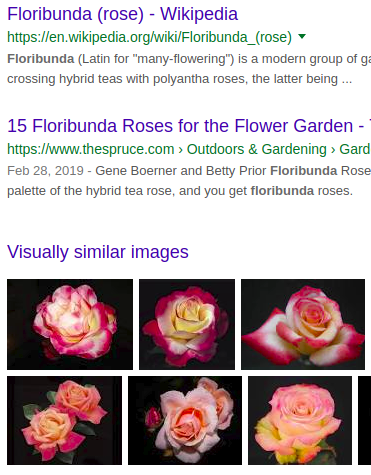
\includegraphics[scale=0.6]{anh_1}
			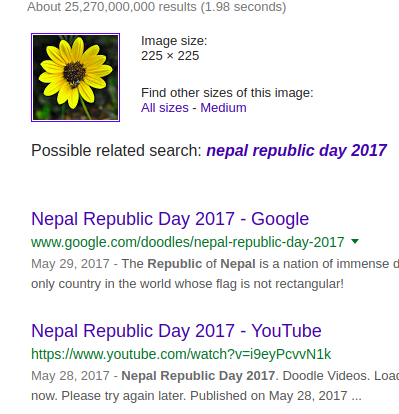
\includegraphics[scale=0.6]{anh_2}
																																																																																																									
			\caption{Ví dụ về tìm kiếm hình ảnh của Google Images}
			\label{fig:anh_1}
		\end{figure}
																																																																						
		\section{Mô tả bài toán nhận dạng hoa}
		Mô tả bài toán: bài toán nhận dạng hoa thông qua ảnh chụp sẽ có đầu vào là một hình ảnh được ghi lại từ các thiết bị ghi hình và đầu ra có thể có hai trường hợp
		\begin{itemize}
			\item \texttt{Trường hợp 1:} Trong ảnh không có hoa thì kết quả trả về là không tồn tại hoa.
			\item \texttt{Trường hợp 2:} Trong ảnh có hoa thì kết quả trả về là một danh sách 5 loài hoa có kết quả nhận dạng tốt nhất.
		\end{itemize}
		Những khó khăn khi nhận diện hoa
		\begin{itemize}
			\item  Số lượng các loài hoa khác nhau mọc trong tự nhiên vô cùng đa dạng và phong phú. Các loài hoa có vô số màu sắc, kiểu dáng hình thù khác nhau gây khó khăn khi phải phân loại với một số lượng loài lớn.
			\item  Các loài hoa đôi khi có kiểu dáng tương đối giống nhau.
			\item  Các loài hoa trong thời gian sinh trưởng có rất nhiều hình thái khác nhau gây ra nhầm lẫn một ví dụ điển hình có thể thấy đó là hoa sen khi chưa nở và lúc đã nở có hình dạng rất khác nhau.
		\end{itemize}
																																																																						
		\begin{figure}[h]
			\centering
			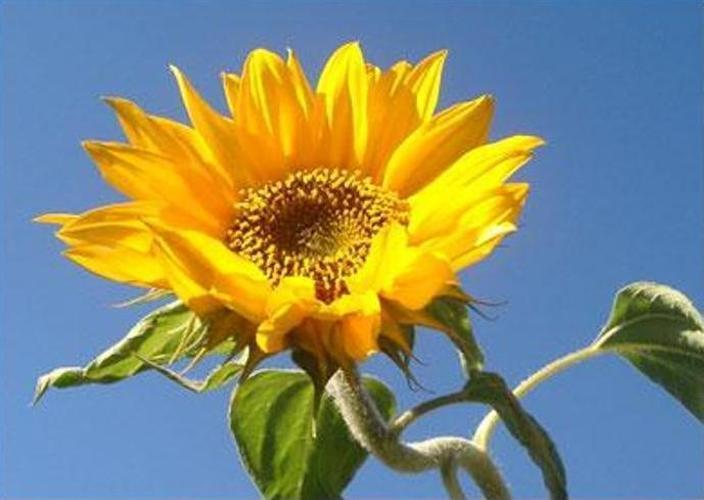
\includegraphics[scale=0.3]{anh_4}
			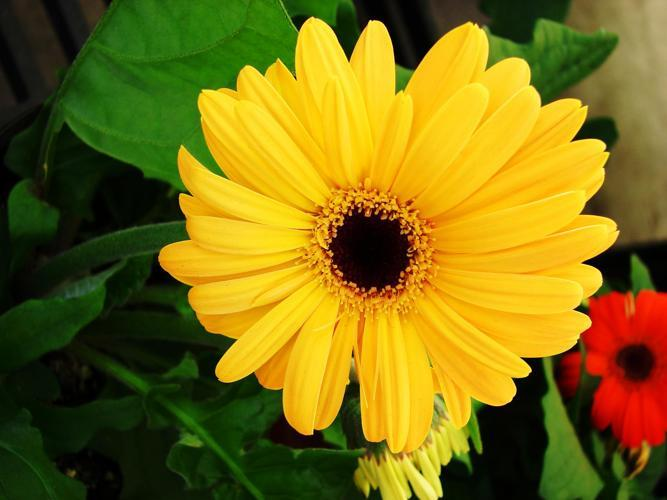
\includegraphics[scale=0.3]{anh_3}
			\caption{Hình ảnh ví dụ về các loài hoa có cấu trúc giống nhau}
			\label{fig:anh_1}
		\end{figure}
		(Ở bên trái là ảnh hoa hướng dương còn ở bên phải là ảnh hoa cúc)
																																																																				
		\begin{figure}[h]
			\centering
			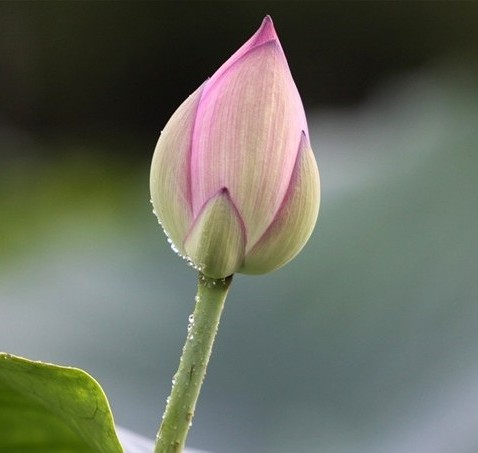
\includegraphics[scale=0.4]{anh_5}
			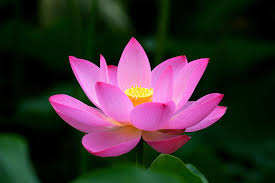
\includegraphics[scale=0.9]{anh_6}
			\caption{Hình ảnh ví dụ về các loài hoa thay đổi hình dạng theo thời gian}
			\label{fig:anh_2}
		\end{figure}
		(Ở bên trái là ảnh hoa sen khi chưa nở còn ở bên phải là ảnh hoa sen khi đã nở)
																																																																						
		\section{Mục tiêu và phương pháp giải quyết vấn đề}
		\subsection{Mục tiêu của khóa luận}
																																																																				
		Mục đích chính của khóa luận này muốn nhắm tới đó là phát triển một ứng dụng nhận dạng tên các loài hoa dành cho người Việt trên nền tảng thiết bị di động. Qua đó cũng đề xuất phương pháp sử dụng mạng học sâu đã được huấn luyện VGG19 [16] trong các mô hình trích xuất thuộc tính từ ảnh, đồng thời tạo tiền đề phát triển cho những nghiên cứu sau này về đề tài nhận diện ảnh.
																																																																		
		Ứng dụng sau khi được phát triển sẽ không đơn thuần chỉ là một công cụ tra cứu mà còn có ý nghĩa trở thành một công cụ học tập, nghiên cứu về thiên nhiên và đặc biệt là các loài hoa giúp các em học sinh, mọi người ở mọi lứa tuổi có thêm một công cụ hữu ích trong việc học tập và nghiên cứu về các loài hoa.
																																																																		
		\subsection{Phương pháp giải quyết bài toán nhận dạng hoa}
																																																																
		Để giải quyết được bài toán nhận dạng tên loài hoa sử dụng ảnh ta cần phải qua năm bước chính đó là:
																																																																
		\begin{itemize}
			\item \texttt{Bước 1:} Tiền xử lý dữ liệu hình ảnh.
			\item \texttt{Bước 2:} Trích xuất các thuộc tính từ ảnh và chuyển thành các vector thuộc tính.
			\item \texttt{Bước 3:} Sử dụng các thuật toán phân loại để phát hiện có hoa trong ảnh hay không.
			\item \texttt{Bước 4:}	Nếu phát hiện thấy hoa trong ảnh thì sử dụng vector thuộc tính đó để nhận dạng tên loài hoa
			\item \texttt{Bước 5}: Tính toán độ tương tự của các ảnh trong tưng loài hoa để đưa ra các ảnh phù hợp nhất cho kết quả.
		\end{itemize}
																																																														
		Qua sự tham khảo các phương pháp trích xuất truyền thống như đã được công bố trong các nghiên cứu [1] [2] và các nghiên cứu gần đây sử dụng mạng tích chập VGG19 [16]. Phương pháp để giải quyết bài toán sẽ diễn ra với các bước sau:
																																																														
		\begin{itemize}
			\item Tiền xử lý hình ảnh bằng phương pháp tách phông nền.
			\item Trích xuất thuộc tính của ảnh sử dụng mạng VGG19 [16]
			\item Xây dựng một mô hình phân loại nhị phân dùng để phát hiện có đối tượng hoa trong ảnh hay không.
			\item Xây dựng một mô hình nhận dạng tên của loài hoa trong ảnh.
			\item Và cuối cùng là một thuật toán tìm kiếm ảnh tương tự khi hiển thị các ảnh kết quả.
		\end{itemize}
																																																								
																																																								
		\subsection{Những điểm mạnh của phương pháp này}
		Qua thực nghiệm và so sánh phương pháp trích xuất thuộc tính sử dụng mô hình học sâu VGG19 [16] với các cách trích xuất thuộc tính truyền thống có kết quả khá khả quan và có tính khả thi cao.
																																																				
		Hơn nữa việc sử dụng lại mô hình trích xuất thuộc tính giữa các bài toán nhận dạng sẽ tiết kiệm được đáng kể công sức cũng như cải thiện được độ chính xác phân loại.
																																																				
		\section{Bố cục các phần trong khóa luận}
		Các phần trong khóa luận được cấu trúc như sau.
																																																				
																																																		
		\begin{itemize}
			\item \textbf{Chương \ref{chap:intro}}: Giới thiệu về bài toán nhận dạng hoa, mục đích và các phương pháp sử dụng để giải quyết bài toán phát triển ứng dụng nhận dạng hoa trên thiết bị di động.
			\item \textbf{Chương \ref{chap:background}}: Trình bày các nghiên cứu liên quan đến bài toán nhận dạng hoa. Các phương pháp trích xuất thuộc tính truyền thống và các phương pháp mới sử dụng mạng học sâu.
			\item \textbf{Chương \ref{chap:solution}}: Trình bày và giải thích về mô hình tổng quát của ứng dụng cũng như cách huấn luyện các mô hình phân loại được sử dụng trong hệ thống.
			\item \textbf{Chương \ref{chap:Experimental results}}: Mô tả về cách thu thập dữ liệu, cách cài đặt và sử dụng các thuật toán để giải quyết vấn đề đồng thời giải thích về mục đích cũng như đưa ra các số liệu thống kê về các kết quả đã đạt được trong từng thí nghiệm. 
			\item \textbf{Chương \ref{chap:conclusion}}: Đưa ra các kết luận về những vấn đề đã giải quyết và những vấn đề chưa giải quyết được đồng thời giới thiệu hướng nghiên cứu để tiếp tục phát triển trong tương lai.	      
		\end{itemize}
																																																				
																																																
																																																		
																																																		
		% chương 2
		\newpage	
		\chapter{Nghiên cứu liên quan đến bài toán nhận dạng hoa}
		\label{chap:background}
																																																						
																																																								
		\section{Các bộ dữ liệu hoa}
		Có khá nhiều các bộ dữ liệu về hoa nổi tiếng và đa dạng ta có thể kể đến như	
		\begin{itemize}
			\item Bộ dữ liệu về hoa của ImageNet.
			\item Oxford-17 [1] bao gồm 1360 ảnh thuộc 17 loài hoa.
			\item Oxford-102 [1] bao gồm 8189 ảnh thuộc 102 loài hoa. 
			\item Kaggle flower dataset: bao gồm 4242 ảnh của 5 loài hoa.
			\item Bộ dữ liệu về thực vật trên trang plant database https://garden.org/plants/.
		\end{itemize}		
																																																				
		Trong khóa luận này sử dụng bộ dữ liệu hoa Oxford-102 [1], vì các lý do sau.
																																																
		\begin{itemize}
			\item Số lượng loài nhiều, số lượng ảnh mỗi loài cũng nhiều.
			\item Các ảnh chụp đều là ảnh chụp cận cảnh bông hoa và đa dạng về góc chụp, ánh sáng.
			\item Các ảnh mỗi loài đều có số lượng loại phong phú, ví dụ ở đây hoa hồng có cả đỏ, hồng, trắng.. thay vì chỉ một loại hoa hồng đỏ.
			\item Có nhiều nghiên cứu sử dụng bộ dữ liệu Oxford-102 \cite{cia-Nilsback06}, cụ thể trong khóa luận có đề cập tới 4 nghiên cứu [1] [2] [3] [4].
		\end{itemize}				
																																																				
		Bộ dữ liệu đã được chia thành bộ huấn luyện bao gồm 10 ảnh mỗi loài hoa, bộ xác nhận bao gồm 10 ảnh mỗi loại và các ảnh còn lại gồm 6129 ảnh làm bộ kiểm tra. 	
																																																		
		\section{Các nghiên cứu phân loại hoa sử dụng bộ hoa của Oxford-102}
		Các nghiên cứu về phân loại hoa [1] [2] [3] [4] có sử dụng bộ dữ liệu hoa Oxford-102 [1] trong đó có thể nhóm lại thành các nhóm theo các phương pháp chính mà các nghiên cứu có sử dụng.
																																														
		\begin{itemize}
			\item Tiền xử lý ảnh trước khi trích xuất thông tin.
			\item Nhận dạng dựa trên vector đặc trưng.
			\item Trích xuất thông tin từ ảnh gốc.
			\item Nhận dạng dựa trên tìm kiếm (retrieval-based).
		\end{itemize}
																																														
		\subsection{Các nghiên cứu về tiền xử lý ảnh trước khi trích xuất thông tin}
		Đầu vào của hệ thống nhận dạng hoa là một bức ảnh được thu lại từ một máy ảnh hoặc các thiết bị ghi hình khác. Các ảnh này đôi khi có chất lượng không như mong muốn, ví dụ như quá tối, chủ thể quá nhỏ, quá to. Nguyên nhân chủ yếu có thể do thiết bị ghi hình không tốt hoặc điều kiện ghi hình không tốt ví dụ trời quá tối, chụp ảnh trong khi đang di chuyển, người chụp ảnh không chú ý. Do vậy để bước phân loại có được kết quả tốt nhất ta cần phải có một bước tiền xử lý ảnh. 
																																												
		Trong nghiên cứu [1] [2] các tác giả sử dụng phương pháp tách phông nền MRF [8]. Theo như hình ảnh dưới đây được lấy trong nghiên cứu [1] các ảnh bên trên là ảnh gốc và các ảnh phía dưới đã được tách phông nền. Ta có thể thấy ở bức ảnh thứ 2 bông hoa sau khi tách phông nền đã bị mất đi 1 phần, tỷ lệ mất mát đối tượng sau tách phông nền theo như báo cáo là 6\%.
																																														
		\begin{figure}[h]
			\centering
			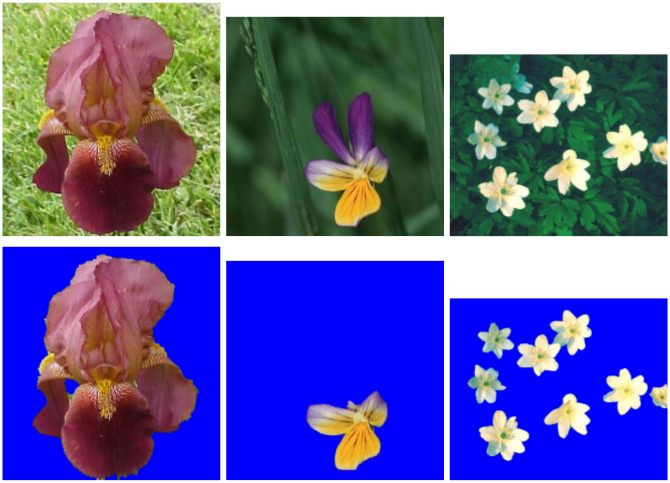
\includegraphics[scale=0.6]{anh_tach_phong_nen}
			\caption{Hình ảnh trong nghiên cứu [1] về phương pháp tách phông nền}
			\label{fig:anh_tach_phong_nen}
		\end{figure}
																																														
		Bên cạnh đó còn một kỹ thuật nữa giúp cải thiện tập dữ liệu là tạo ra nhiều dữ liệu hơn từ dữ liệu ban đầu. Đối với xử lý ảnh, kỹ thuật này có tên là ảnh mở rộng (Image Augmentation) [11] [17] . Ví dụ như sau, chúng ta có một bông hoa hồng thì khi soi vào gương, dịch sang trái, phải, trên, dưới, đứng trong tối, ngoài sáng, phóng to, thu nhỏ, xoay 1 góc bất kỳ thì cũng vẫn là một bông hồng đó. Vậy thì từ một ảnh huấn luyện, ta có thể tạo ra vô vàn những ảnh tương tự và vẫn có thể được nhận ra là bông hồng bằng các phép biến đổi ảnh như: xoay ảnh, lật ảnh, dịch ảnh,.. Và như vậy, chúng ta có một tập dữ liệu lớn hơn cho bước huấn luyện. Nghiên cứu [4] có sử dụng phương pháp này và đã tăng được độ chính xác từ 74,4\% lên thành 86.8\%
																																														
		\subsection{Các nghiên cứu về nhận dạng dựa trên vector đặc trưng}
																																												
		Trích xuất thông tin là một phương pháp từ các dữ liệu thô ban đầu chuyển thành các tập, thuộc tính giúp chúng ta biểu diễn tập dữ liệu ban đầu tốt hơn. Cụ thể trong bài toán trích xuất thông tin từ ảnh ta có dữ liệu đầu vào là một hình ảnh, hay nói cách khác là một tập hợp biểu diễn các điểm ảnh. Tùy vào các mục đích khác nhau ta sẽ có những phương pháp trích xuất thuộc tính riêng biệt.
																																												
		Nghiên cứu [1] sử dụng phương pháp trích xuất các đặc trưng phổ biến của một bức ảnh bao gồm màu sắc, khối hình và hoa văn từ đó sử dụng phương pháp láng giềng gần nhất để phân loại ra tên của loài hoa đó. Kết quả phân loại tốt nhất đạt được bằng cách kết hợp hình dạng và màu sắc đạt kết quả 81.3\%
																																												
																																												
																																										
		\begin{table}[h]
			\centering
			\caption{Bảng kết quả của nghiên cứu [2]}
			\label{tbl:table ket qua cua Nilsback08}
			\begin{tabular}{|l|c|}
				\hline
				\textbf{Thuộc tính trích xuất}      & \textbf{Độ chính xác phân loại (\%)} \\ \hline
				HSV                                       & 43.0                                         \\ \hline
				SIFT internal                             & 55.1                                         \\ \hline
				SIFT boundary                             & 32.0                                         \\ \hline
				HOG                                       & 49.6                                         \\ \hline
				HSV + SIFT internal                       & 66.4                                         \\ \hline
				HSV + SIFT boundary                       & 57.0                                         \\ \hline
				HSV + HOG                                 & 62.1                                         \\ \hline
				SIFT internal + HOG                       & 66.4                                         \\ \hline
				SIFT boundary + HOG                       & 55.3                                         \\ \hline
				HSV + SIFT internal + HOG                 & 71.8                                         \\ \hline
				HSV + SIFT internal + SIFT boundary + HOG & 72.8                                         \\ \hline
																																																																																				
			\end{tabular}
		\end{table}
																																												
		Bảng \ref{tbl:table ket qua cua Nilsback08} cho thấy các kết quả của nghiên cứu \cite{cia-Nilsback08}, tại đó các tác giả đã tính toán bốn đặc điểm khác nhau cho các bông hoa, cụ thể là hình dạng kết cấu cục bộ, hình dạng của ranh giới, phân bố không gian tổng thể của cánh hoa và màu sắc của các loài hoa. Sau đó kết hợp các tính năng bằng cách sử dụng phân loại SVM. Kết quả cho thấy độ chính xác phân loại cho các bộ thuộc tính khác nhau. Có thể thấy rằng việc kết hợp tất cả các thuộc tính mang lại độ chính xác tốt hơn nhiều so với sử dụng các thuộc tính đơn lẻ.
																																				
		\textbf{Vector đặc trưng về khối hình}
																														
		Theo thứ tự từ trái qua phải: hoa gió, hoa buttercup và hoa thủy tiên. Nhìn qua thì các loài hoa này có cấu trúc tương tự nhau nhưng lại không hoàn toàn giống nhau. Sử dụng các mô tả SIFT [6] trên một lưới thông thường độ rộng của lưới M điểm ảnh, với phạm vi từ 10 đến 70 pixel, khu vực hỗ trợ cho Tính toán SIFT với bán kính R dao động từ 10 đến 70 pixel.				 
																																							
		\begin{figure}[h]
			\centering
			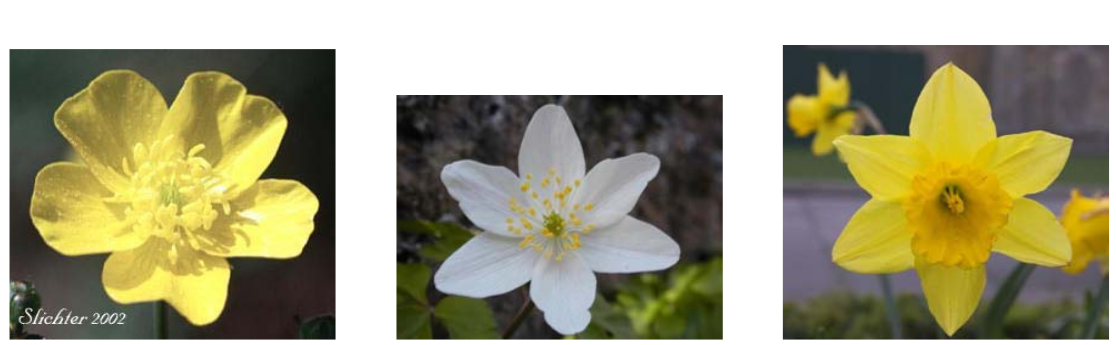
\includegraphics[scale=0.3]{anh_hoa_hinh_dang}
			\caption{Hình ảnh trong nghiên cứu \cite{cia-Nilsback06} về các loài hoa có hình dáng tương tự nhau}
			\label{fig:anh_hoa_hinh_dang}
		\end{figure}						 
																																										 
																																							
		\textbf{Vector đặc trưng về kết cấu trên vùng tiền cảnh sử dụng SIFT}	
																														
		Các mô tả SIFT được tính toán tại các điểm trên một lưới thông thường với khoảng cách M điểm ảnh trên vùng hoa tiền cảnh. Tại mỗi điểm lưới, các bộ mô tả được tính toán trên các cửa sổ hỗ trợ hình tròn với bán kính R điểm ảnh kết quả thu được là một vectơ 128 chiều.						 
																														
																																						 
		\textbf{Vector đặc trưng kết cấu trên vùng ranh giới sử dụng SIFT}												
																														
		Ranh giới của ảnh sau bước tiền xử lý tách phông nền cho ta ranh giới của hoa. Sau đó lấy mẫu các mô tả SIFT trên đường viền của bông hoa, chúng ta có thể nhấn mạnh hơn đến hình dạng cục bộ của đường biên. Sử dụng các cửa sổ hình tròn bán kính R điểm ảnh và bước nhảy S điểm ảnh dọc theo đường biên của bông hoa kết quả thu được cũng thu được một vector 128 chiều.							
																																								
																														
		\textbf{Vector đặc trưng về màu sắc}
																												
		Một số hoa có màu sắc rất đặc trưng và có thể giúp thu hẹp đáng kể các loài để phân loại, nhưng nó sẽ không cho phép chúng ta xác định chính xác các loài hoa. Sử dụng mô tả màu bằng không gian màu HSV để giảm hiệu ứng của ánh sáng môi trường tới ảnh.
																										
		\textbf{Vector đặc trưng về hoa văn}
		Một số hoa có hoa văn đặc trưng trên cánh hoa của chúng. Những họa tiết này có thể đặc biệt hơn, chẳng hạn các sọc của hoa păng xê, các ô vuông ở hoa đầu rắn, hoặc các chấm nhỏ ở hoa ly hổ
		\begin{figure}[h]
			\centering
			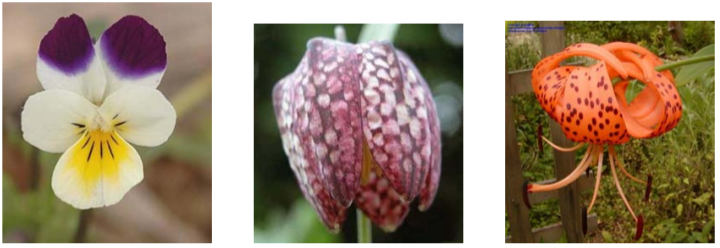
\includegraphics[scale=0.5]{anh_hoa_cau_truc}
			\caption{Hình ảnh trong nghiên cứu \cite{cia-Nilsback06} về các loài hoa có hình dáng tương tự nhau}
			\label{fig:anh_hoa_cau_truc}
		\end{figure}
																								
		Sử dụng bộ lọc MR8 [12] với vùng hỗ trợ hình vuông có kích thước từ 3 đến 19 pixel.Kết quả trên cho thấy độ chính xác phân loại thay đổi theo số lượng cụm cho các kích thước bộ lọc khác nhau.
																								
		\textbf{Vector đặc trưng về phân bố tổng thể}
																								
		Sử dụng phương pháp HOG [7] , tương tự như các tính năng SIFT, ngoại trừ việc chúng sử dụng tương phản cục bộ chồng chéo đã chuẩn hóa giữa các ô trong một lưới. Tuy nhiên, thay vì được áp dụng cho các vùng cục bộ (bán kính R trong trường hợp SIFT), HOG được áp dụng ở đây trên toàn bộ vùng hoa. Theo cách này, sẽ mô tả được sự phân bố không gian toàn cầu của hoa.
																								
		% \newpage
		\subsection{Nghiên cứu về trích xuất thông tin từ ảnh gốc}
																								
		\textbf{Mạng tích chập OverFeat [4]}
		Trong nghiên cứu này [4] các tác giả sử dụng mạng tích chập có tên là OverFeat. Mỗi lớp tích chập có chứa 96 đến 1024 các cửa sổ tích chập có kích thước 3 x 3 đến 7 x 7. Chỉnh lưu nửa sóng được sử dụng làm chức năng kích hoạt phi tuyến. Các hạt nhân gộp tối đa (Max polling) có kích thước 3 x 3 và 5 x 5 được sử dụng ở các lớp khác nhau. Mô hình nhận đầu vào là hình ảnh màu có kích thước 221 x 221. OverFeat đã được đào tạo cho nhiệm vụ phân loại hình ảnh của ImageNet ILSVRC 2013 và thu được kết quả khá cao.
																						
		Các tác giả sử dụng bộ dữ liệu ImageNet ILSVRC13 chứa 1,2 triệu hình ảnh được dán nhãn bằng tay của 1000 loại nhãn để huấn luyện cho mô hình. Sau đó có thử nghiệm trên bộ dữ liệu [2] và thu được kết quả như bảng sau.
																						
		\begin{table}[h]
			\centering
			\caption{Bảng kết quả của nghiên cứu \cite{cia-CNNFeatures off-the-shelf}}
			\label{tbl:table ket qua cua Nilsback08}
			\begin{tabular}{|l|c|}
				\hline
				\textbf{Phương pháp} & \textbf{Độ chính xác phân loại (\%)} \\ \hline
				CNN-SVM w/o seg         & 74.7                                         \\ \hline
				CNNaug-SVM w/o seg      & 86.8                                         \\ \hline
																																																																																				
			\end{tabular}
		\end{table}
																				
		Đối với tất cả các thí nghiệm đều sử dụng đến lớp kết nối đầy đủ đầu tiên (lớp 22) của mạng để cho ra vector thuộc tính. Đối với tất cả các thử nghiệm, thay đổi kích thước toàn bộ hình ảnh thành 221 x 221. Đầu ra sẽ cho một vector thuộc tính có 4096 chiều. Trong nghiên cứu có đề cập tới hai loại cài đặt là có sử dụng phương pháp tăng cường ảnh CNNaug và không sử dụng phương pháp tăng cường ảnh. Đối với các nhu cầu phân loại trong đó các nhãn không loại trừ lẫn nhau các tác giả sử dụng chiến lược một với tất cả (one-against-all), và trong phần còn lại của các thí nghiệm sử dụng các SVM tuyến tính một đối một (one-against-one).
																				
																				
		\textbf{Mạng tích chập VGG19 \cite{cia_vgg19}}
																						
		Dựa trên các công trình nghiên cứu trước đó thì vào năm 2015 có một nghiên cứu [16] đề xuất sử dụng mạng tích chập ConvNet [16] gồm rất nhiều lớp để có thể đáp ứng được khả năng phân loại trên diện rộng. Trong nghiên cứu này, các tác giả đã điều tra ảnh hưởng của độ sâu mạng tích chập đến độ chính xác trong việc nhận dạng hình ảnh với quy mô lớn.  
																						
		Qua đánh giá kỹ lưỡng các mạng đã được tăng độ sâu bằng cách sử dụng kiến trúc với các bộ lọc tích chập rất nhỏ (3 x 3), cho thấy có thể đạt được sự cải thiện đáng kể về cấu hình trước khi nâng độ sâu lên 16 đến 19 lớp.
																						
		Dưới đây là mô tả cách cài đặt cho mạng ConvNet. Độ sâu của các cấu hình tăng từ trái (A) sang phải (E), khi nhiều lớp được thêm vào (các lớp được thêm vào được in đậm). Các tham số của lớp tích chập được ký hiệu là kích thước trường xác nhận kích thước của bộ dữ liệu của kênh. Kết quả thu được là một vector thuộc tính 4096 chiều.
																						
		\begin{figure}[h]
			\centering
			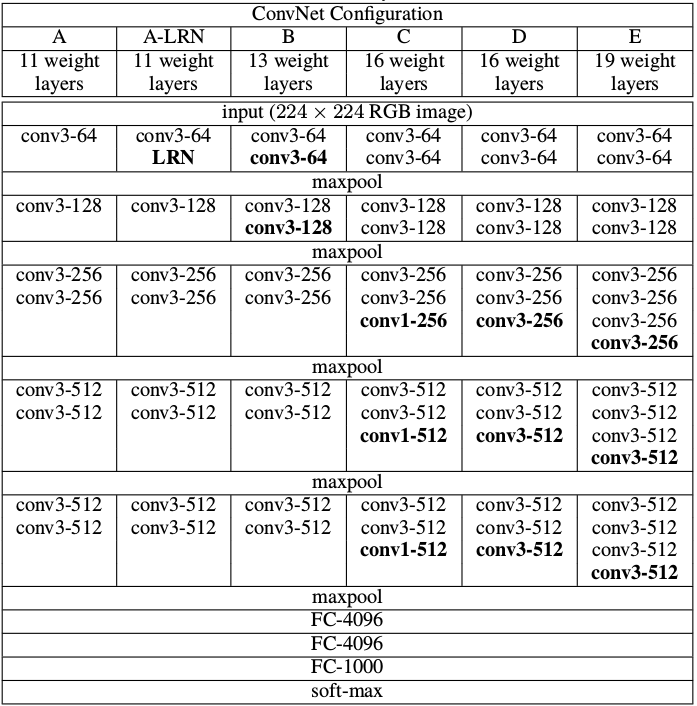
\includegraphics[scale=0.6]{vgg19_table}
			\caption{Bảng mô tả cài đặt cho mạng VGG19 trong nghiên cứu \cite{cia_vgg19} }
			\label{fig:vgg19_table}
		\end{figure}
																				
		\begin{figure}[h]
			\centering
			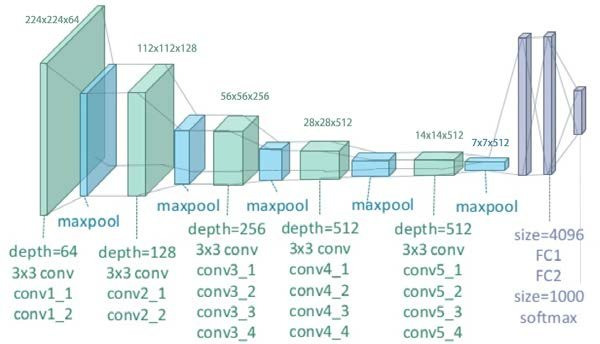
\includegraphics[scale=0.7]{vgg19_image}
			\caption{Hình ảnh mô tả kiến trúc của VGG19 lấy từ trang www.researchgate.net}
			\label{fig:vgg19_image}
		\end{figure}
																						
		\subsection{Nghiên cứu về nhận dạng ảnh dựa trên tìm kiếm}
																						
		Phương pháp nhận dạng ảnh dựa trên tìm kiếm có chút khác biệt so với bài toán phân loại hình ảnh, đầu vào của bài toán vẫn là một hình ảnh và nhiệm vụ đặt ra ở đây là phải sắp xếp, hoặc tìm kiếm, những hình ảnh có liên quan trong cơ sở dữ liệu. Có hai hướng tiếp cận trong bài toán truy hồi là theo hướng khái niệm và hướng nội dung.
																				
		\begin{itemize}
			\item Tiếp cận theo hướng khái niệm: là việc tìm kiếm dựa trên các thông tin liên quan đến một bức ảnh như tên bức ảnh, tiêu đề, chủ đề hoặc phần chữ miêu tả về bức ảnh đó.
			\item Tiếp cận theo hướng nội dung: là việc tìm kiếm dựa trên nội dung của ảnh.
		\end{itemize}
		Nghiên cứu về nhận dạng hoa có sử dụng phương pháp tìm kiếm hình ảnh [3] tại đây các tác giả sử dụng thuật toán ước lượng láng giềng gần nhất trực tiếp (Online Nearest neighbor Estimation - ONE) cho cả phân loại và truy hồi hình ảnh, bằng cách tính độ tương tự giữa các đối tượng trong ảnh dùng để tìm kiếm với từng lớp hoặc các hình ảnh của lớp đó. Kết quả phân loại tốt nhất mà các tác giả đạt được trên bộ dữ liệu [2] là 86.24\%
																				
		\textbf{Các bước thực hiện của phương pháp}
		\begin{figure}[h]
			\centering
			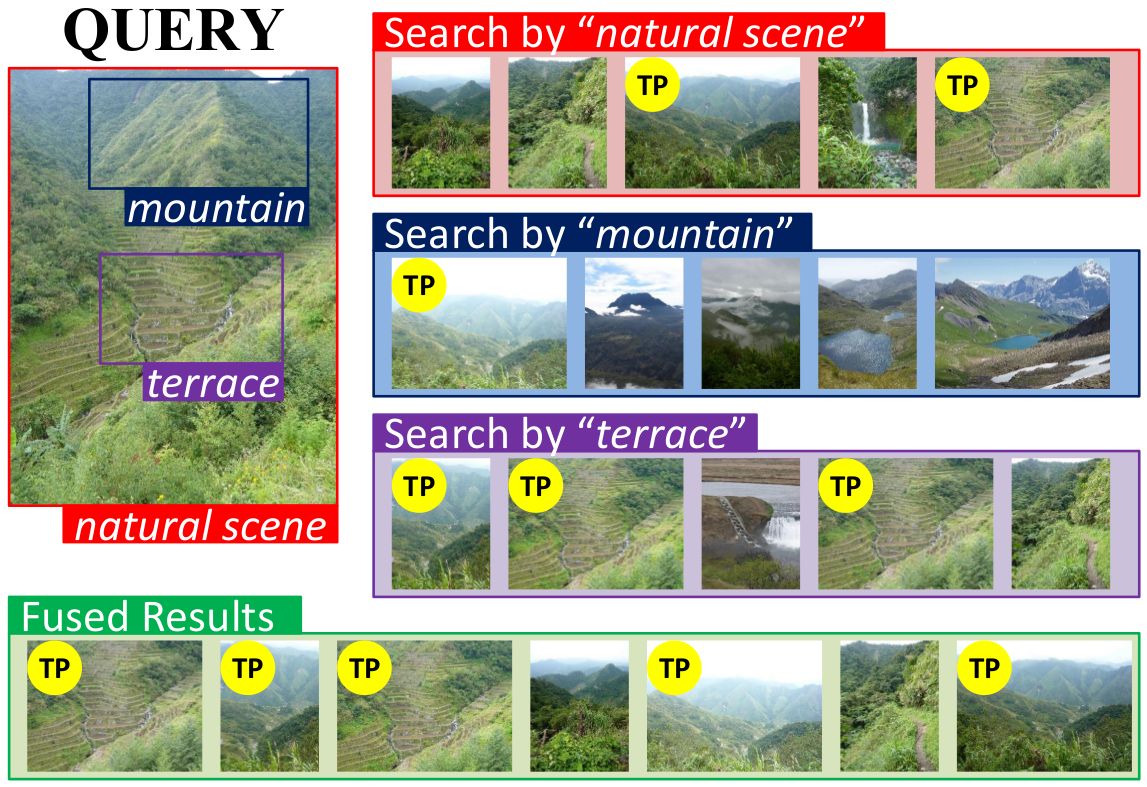
\includegraphics[scale=0.4]{one}
			\caption{Hình ảnh tóm tắt về phương pháp ước lượng láng giềng gần nhất trong nghiên cứu [3] của tác giả}
			\label{fig:one}
		\end{figure}
																		
		Đầu tiên sử dụng phương pháp phát hiện đa vật thể dựa theo các nghiên cứu [13] [14] [15] trên hình ảnh truy vấn và từng hình ảnh của các lớp. Ở đây hình ảnh bên trái ở trên là hình ảnh cần tìm kiếm ta sẽ sử dụng phương pháp pháp hiện đa vật thể ra được các vật thể có trong bức ảnh là "mountain", "terrace" và "natural scene".
																		
		Trong bộ dữ liệu của ta, ta sẽ lấy ra các lớp về "mountain", "terrace" và "natural scene". Rồi sau đó trích xuất các thuộc tính trên mỗi đối tượng đó để cung cấp một mô tả sát nhất cho hình ảnh tìm kiếm. 
																		
		So sánh mức độ liên quan giữa các đối tượng đã được phát hiện trong ảnh truy vấn với các đối tượng trong các ảnh thành viên trong lớp đó. Các ảnh nào có độ tương tự gần nhất với các đối tượng có mặt trong hình ảnh cần tìm kiếm sẽ có chữ "TP - true positive" màu vàng.
																		
		Trong bước tìm kiếm, mức độ liên quan của hình ảnh cần tìm kiếm đối với một danh mục hoặc hình ảnh ứng cử viên được tính bằng mức trung bình gần nhất khoảng cách từ hình ảnh cần tìm kiếm đối tượng đến các đối tượng trong lớp đó.
																		
		\section{Các ứng dụng di động cho nhận dạng hoa}
																
		Các ứng dụng nhận dạng hoa và thực vật có xuất hiện khá nhiều nhưng lại có sự khác biệt khá lớn về độ chính xác và tốc độ nhận dạng. Trong khóa luận này lấy ra 3 ví dụ về ứng dụng nhận dạng hoa có độ chính xác và tốc độ nhận dạng khá tốt.
																
																		
																
		\begin{itemize}
			\item PictureThis - Flower \& Plant Identification: do công ty Glority Software Limited.	
			\item PlantNet Plant Identification: do công ty plantnet-project.org.
			\item PlantFinder - Flower \& Plant Identification: do công ty HD Wallpapers Production. 		
		\end{itemize}
																
		\begin{figure}[h]
			\centering
			
\includegraphics[scale=0.7]{picture_this_app}
			
\includegraphics[scale=0.7]{plantnet_app}
			
\includegraphics[scale=0.7]{plantfinder_app}
			\caption{Hình ảnh đại diện của các ứng dụng}
			\label{fig:app_curent}
		\end{figure}
		(Lần lượt từ trái qua phải ta có các ứng dụng là PictureThis, PlantNet, PlantFinder)
		Ưu điểm chung của các ứng dụng:
		\begin{itemize}
			\item Các ứng dụng có độ nhận dạng chính xác khá tốt.
			\item Thời gian phản hồi ở mức khá.
			\item Có nêu ra đặc điểm chi tiết của loài hoa.
		\end{itemize}
		Một số nhược điểm còn tồn tại:
		\begin{itemize}
			\item Toàn bộ tên loài hoa và chi tiết về đặc điểm của loài hoa đang ở tiếng anh và tiếng latin, gây ra đôi chút khó khăn cho người Việt khi cần tra cứu.
			\item Một số ứng dụng sau khi chụp xong cần phải khoanh vùng hoa cần tìm bằng tay, chưa tự động phát hiện.
			\item Một số ứng dụng chưa có bước phát hiện xem ảnh có hoa hay không.
		\end{itemize}
														
		\begin{figure}[h]
			\centering
			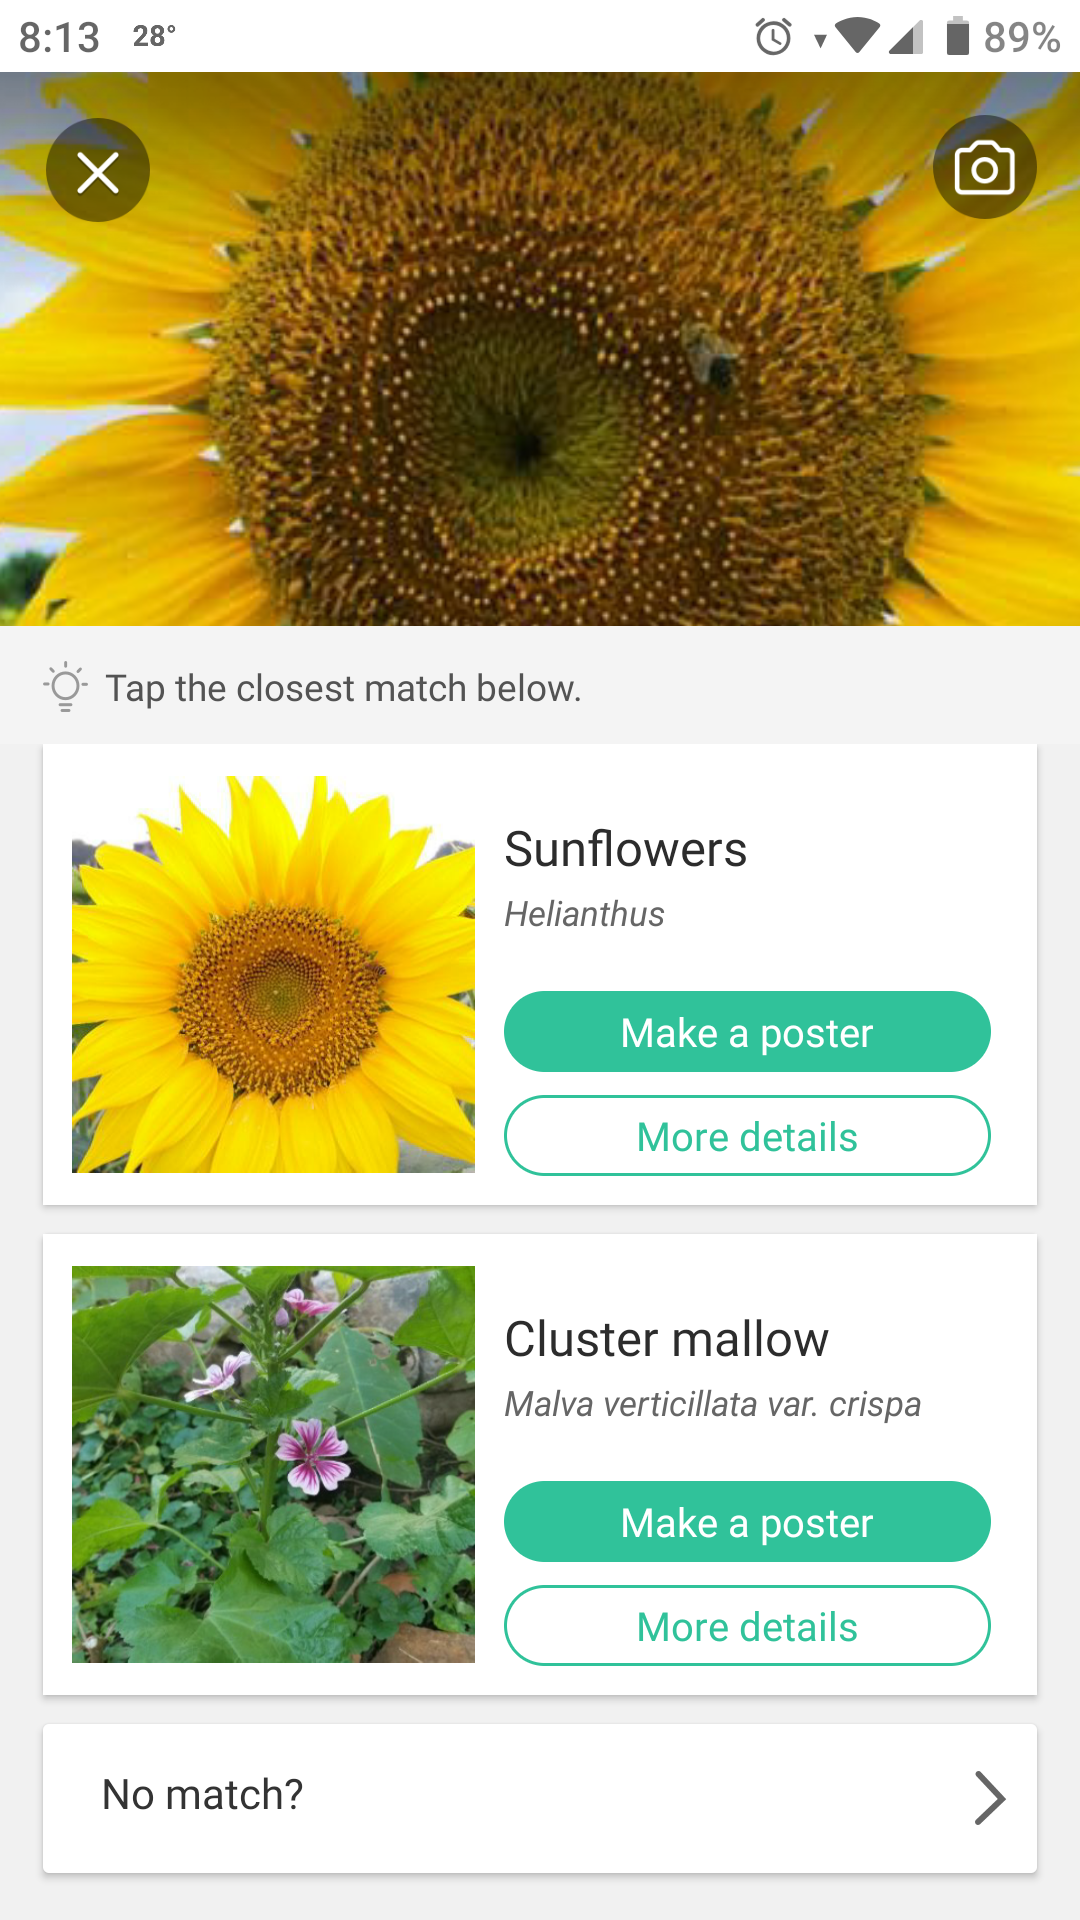
\includegraphics[scale=0.13]{app_en_1}
			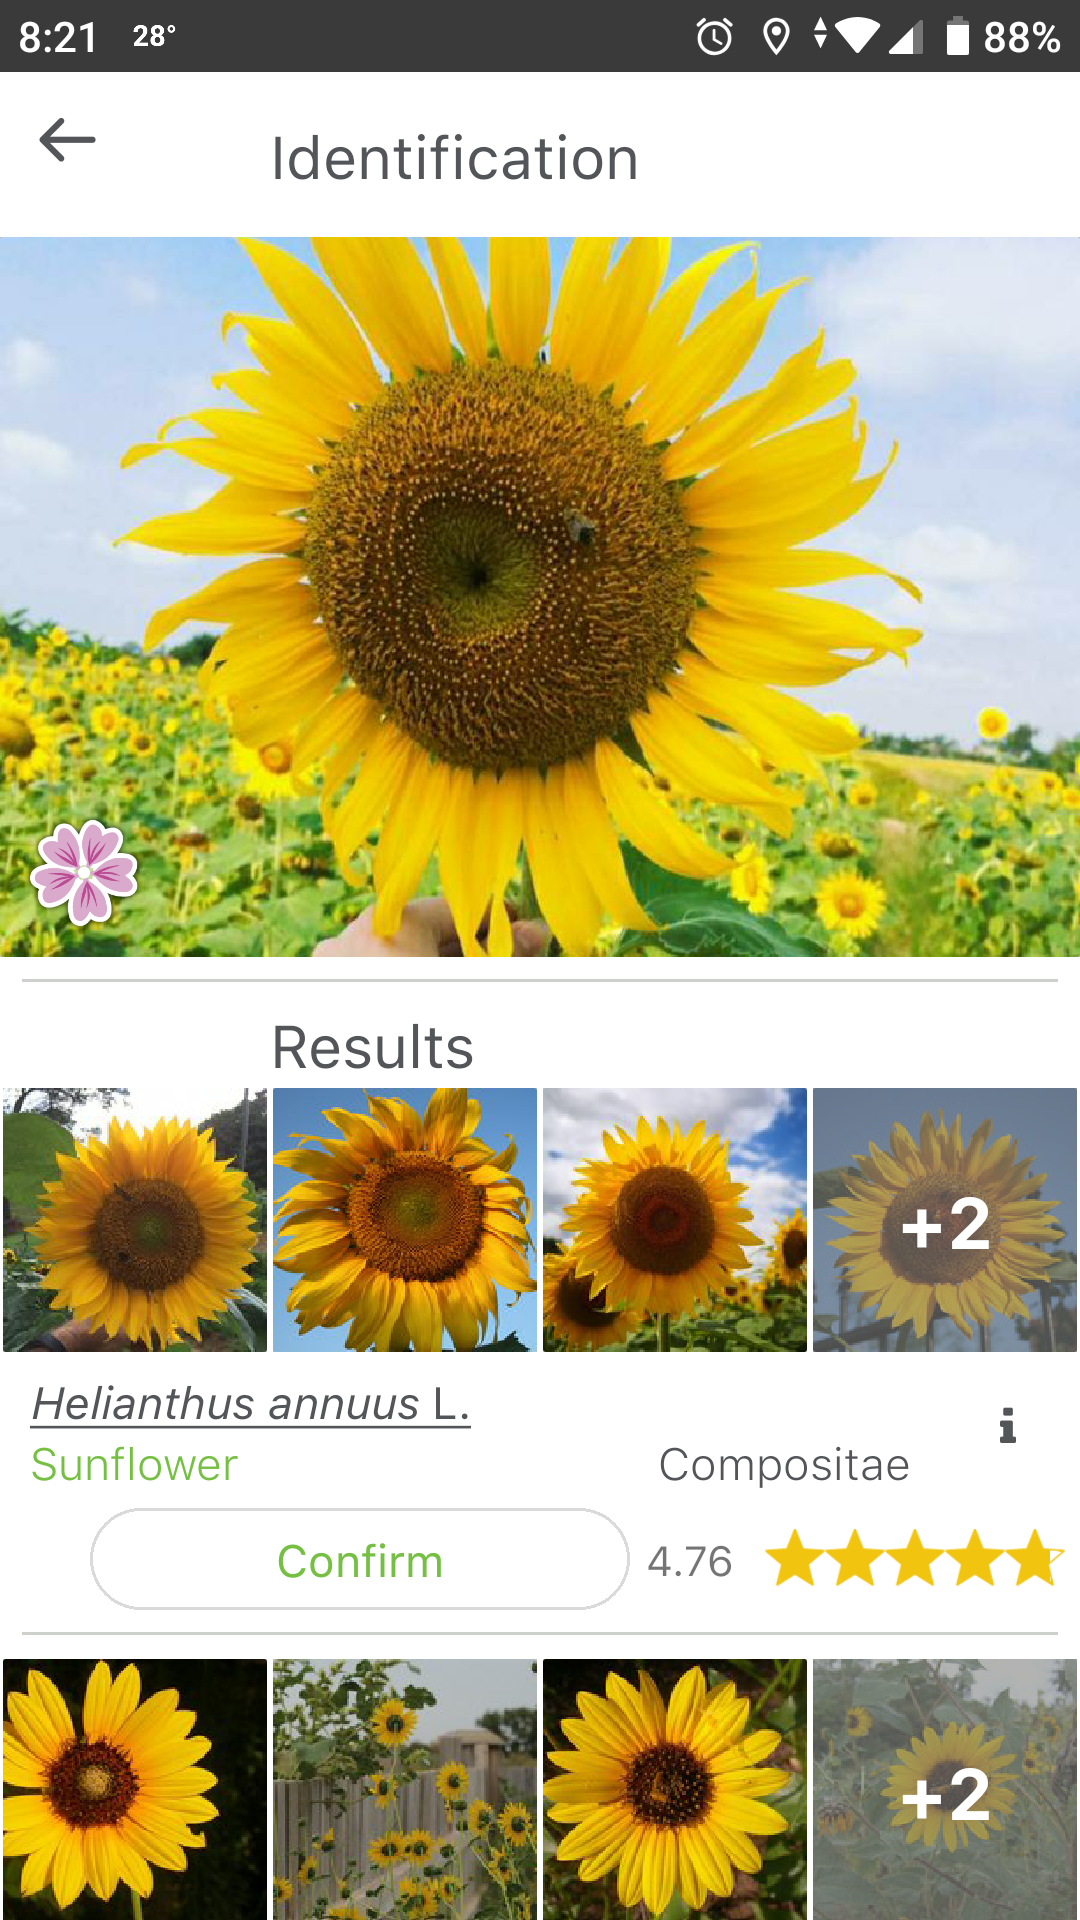
\includegraphics[scale=0.13]{app_en_2}
			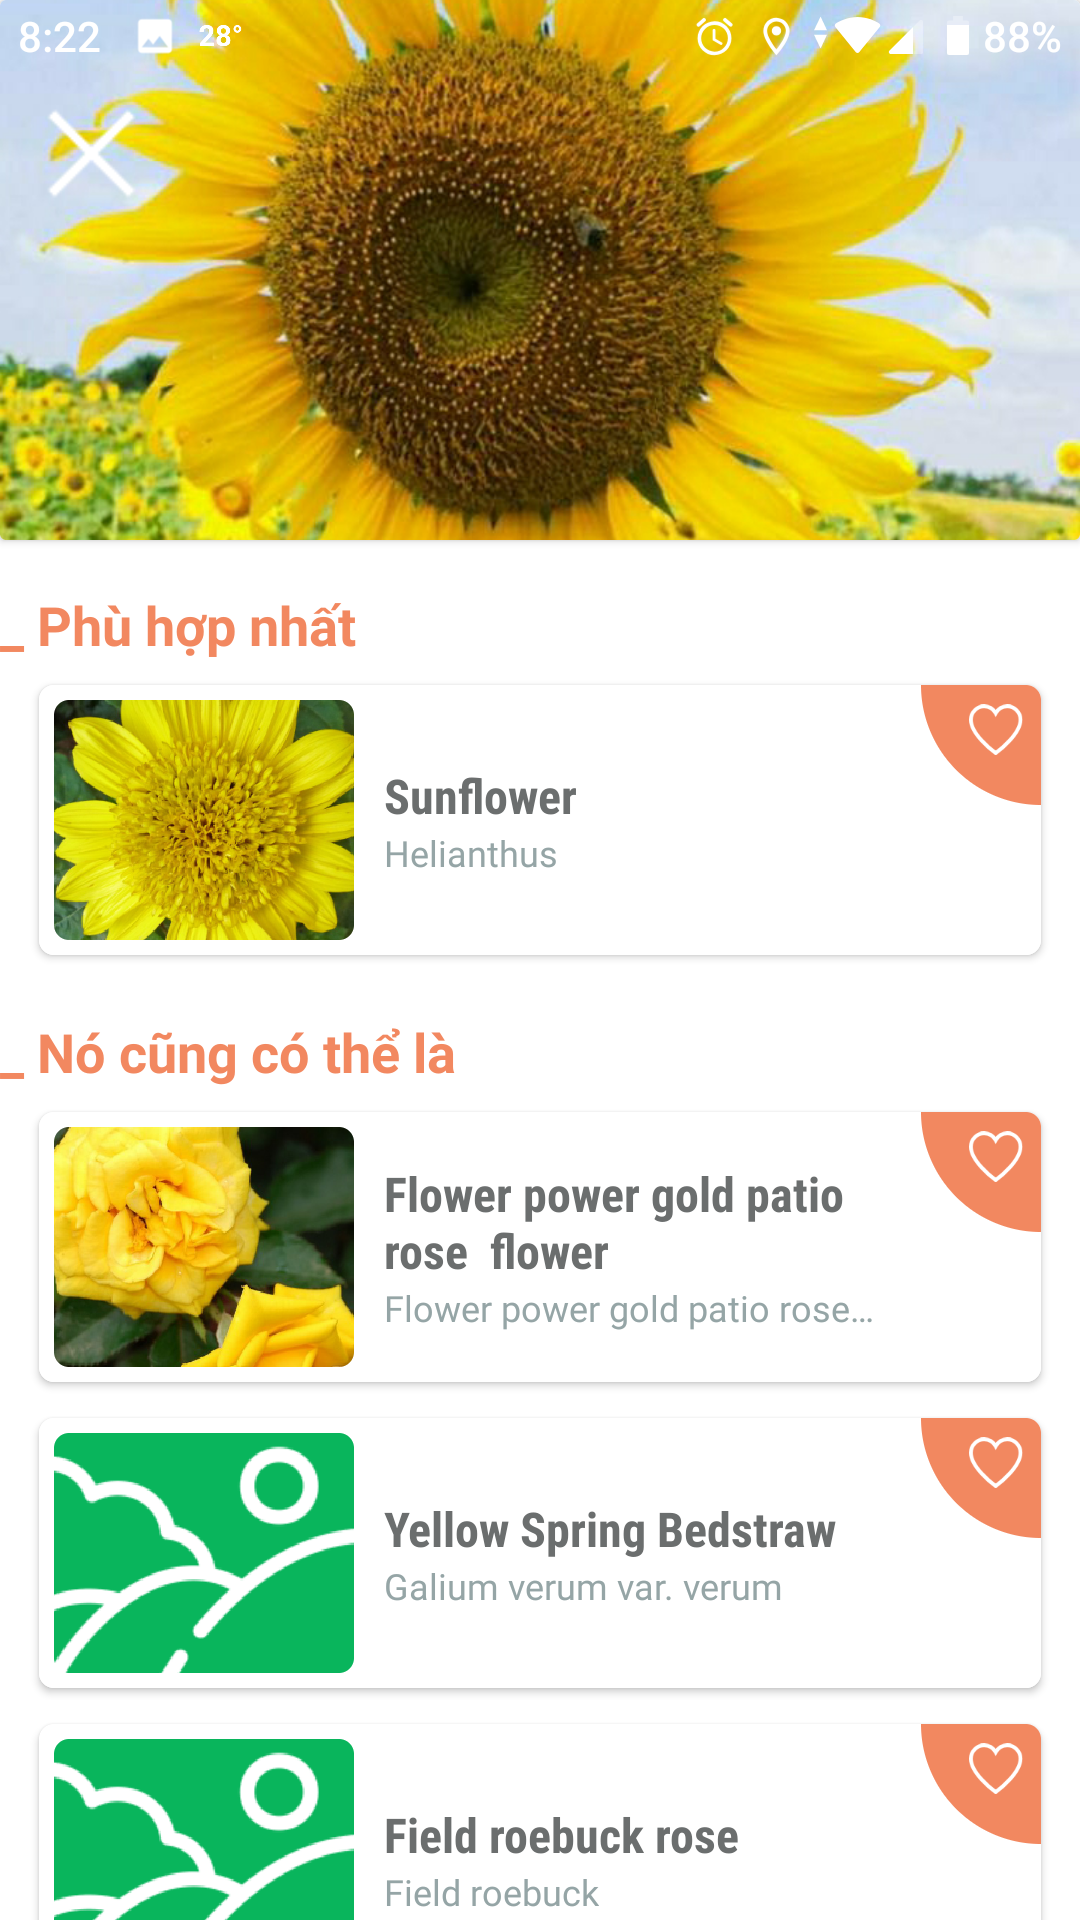
\includegraphics[scale=0.13]{app_en_3}
			\caption{Hình ảnh kết quả toàn tiếng Anh khi tra cứu ảnh hoa hướng dương bằng các ứng dụng}
			\label{fig:app_en}
		\end{figure}
		(Lần lượt từ trái qua phải là ảnh chụp màn hình kết quả của các ứng dụng PlantFinder, PlantNet và cuối cùng là Picture this.)
																
		\begin{figure}[h]
			\centering
			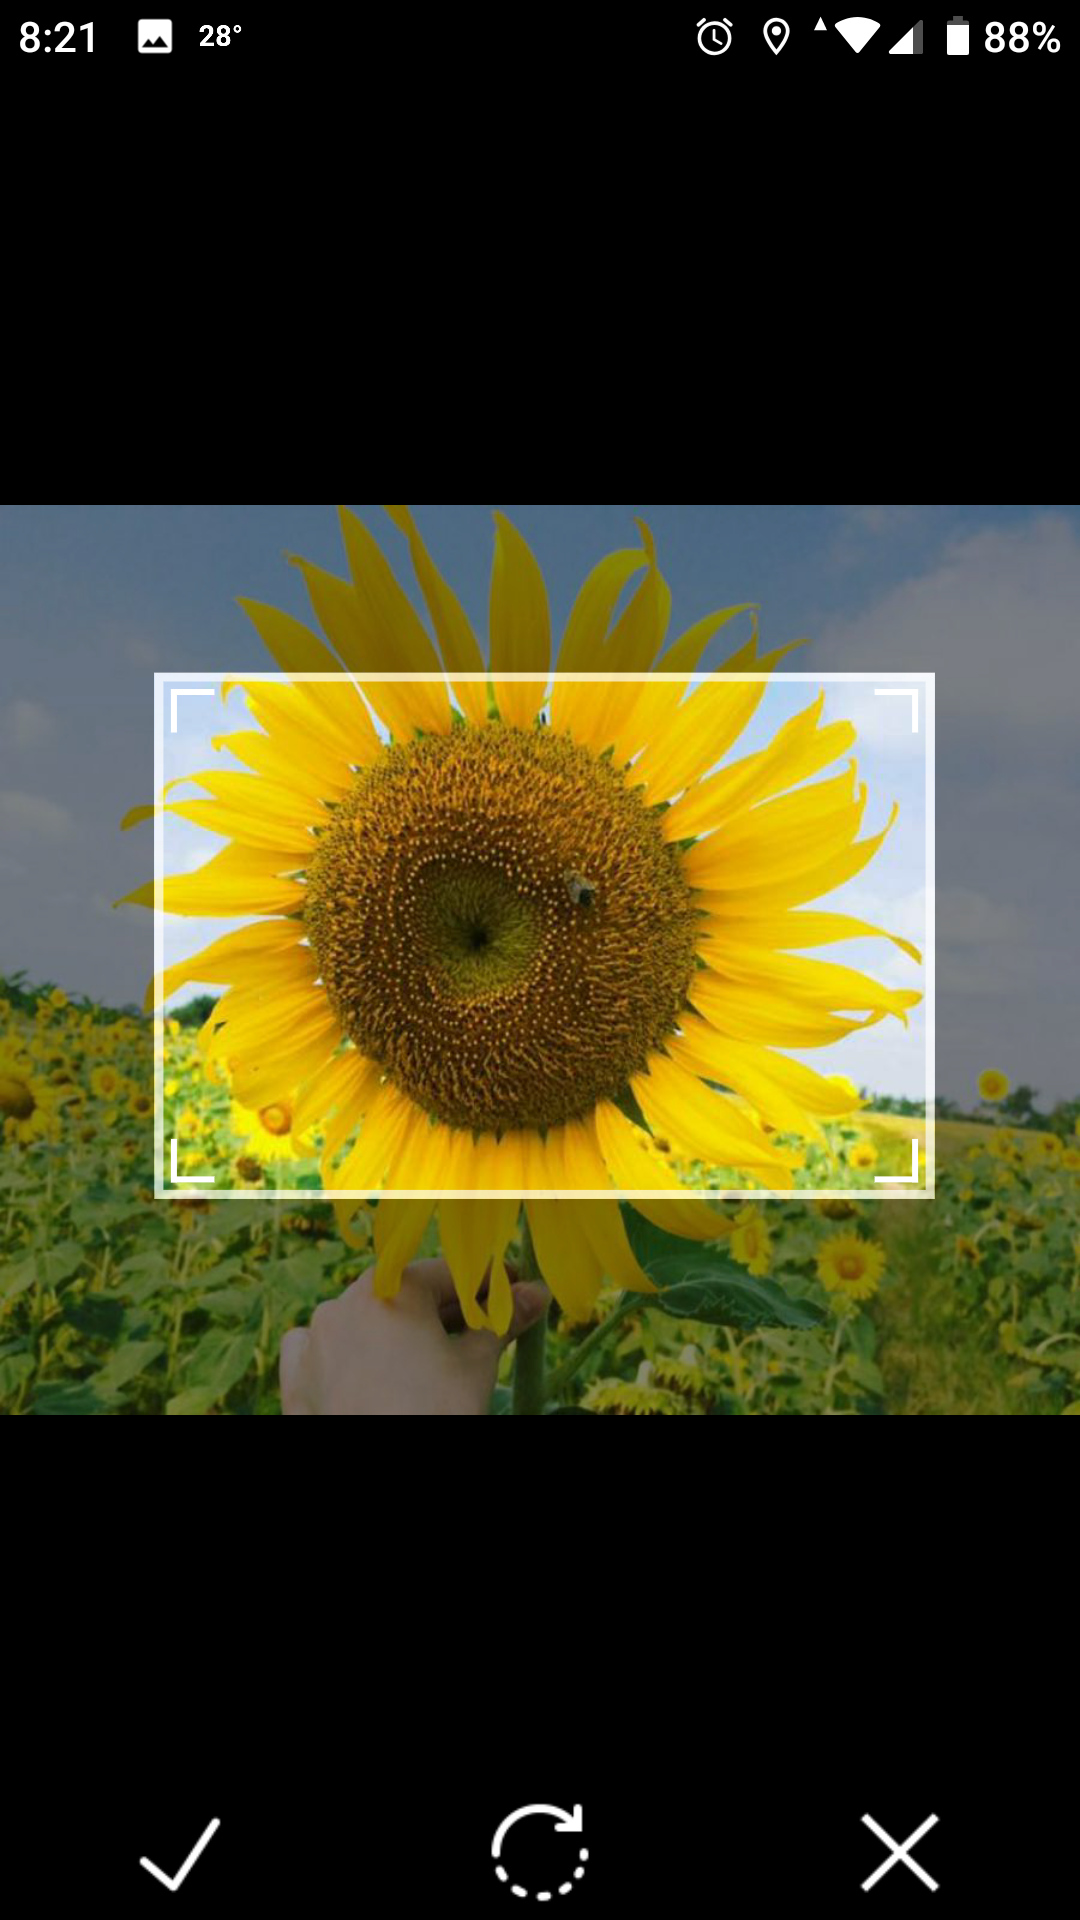
\includegraphics[scale=0.13]{app_1}
			\caption{Hình ảnh về ứng dụng PlantFinder cần phải khoanh vùng phần có hoa bằng tay}
			\label{fig:app_1}
		\end{figure}
														
		\begin{figure}[h]
			\centering
			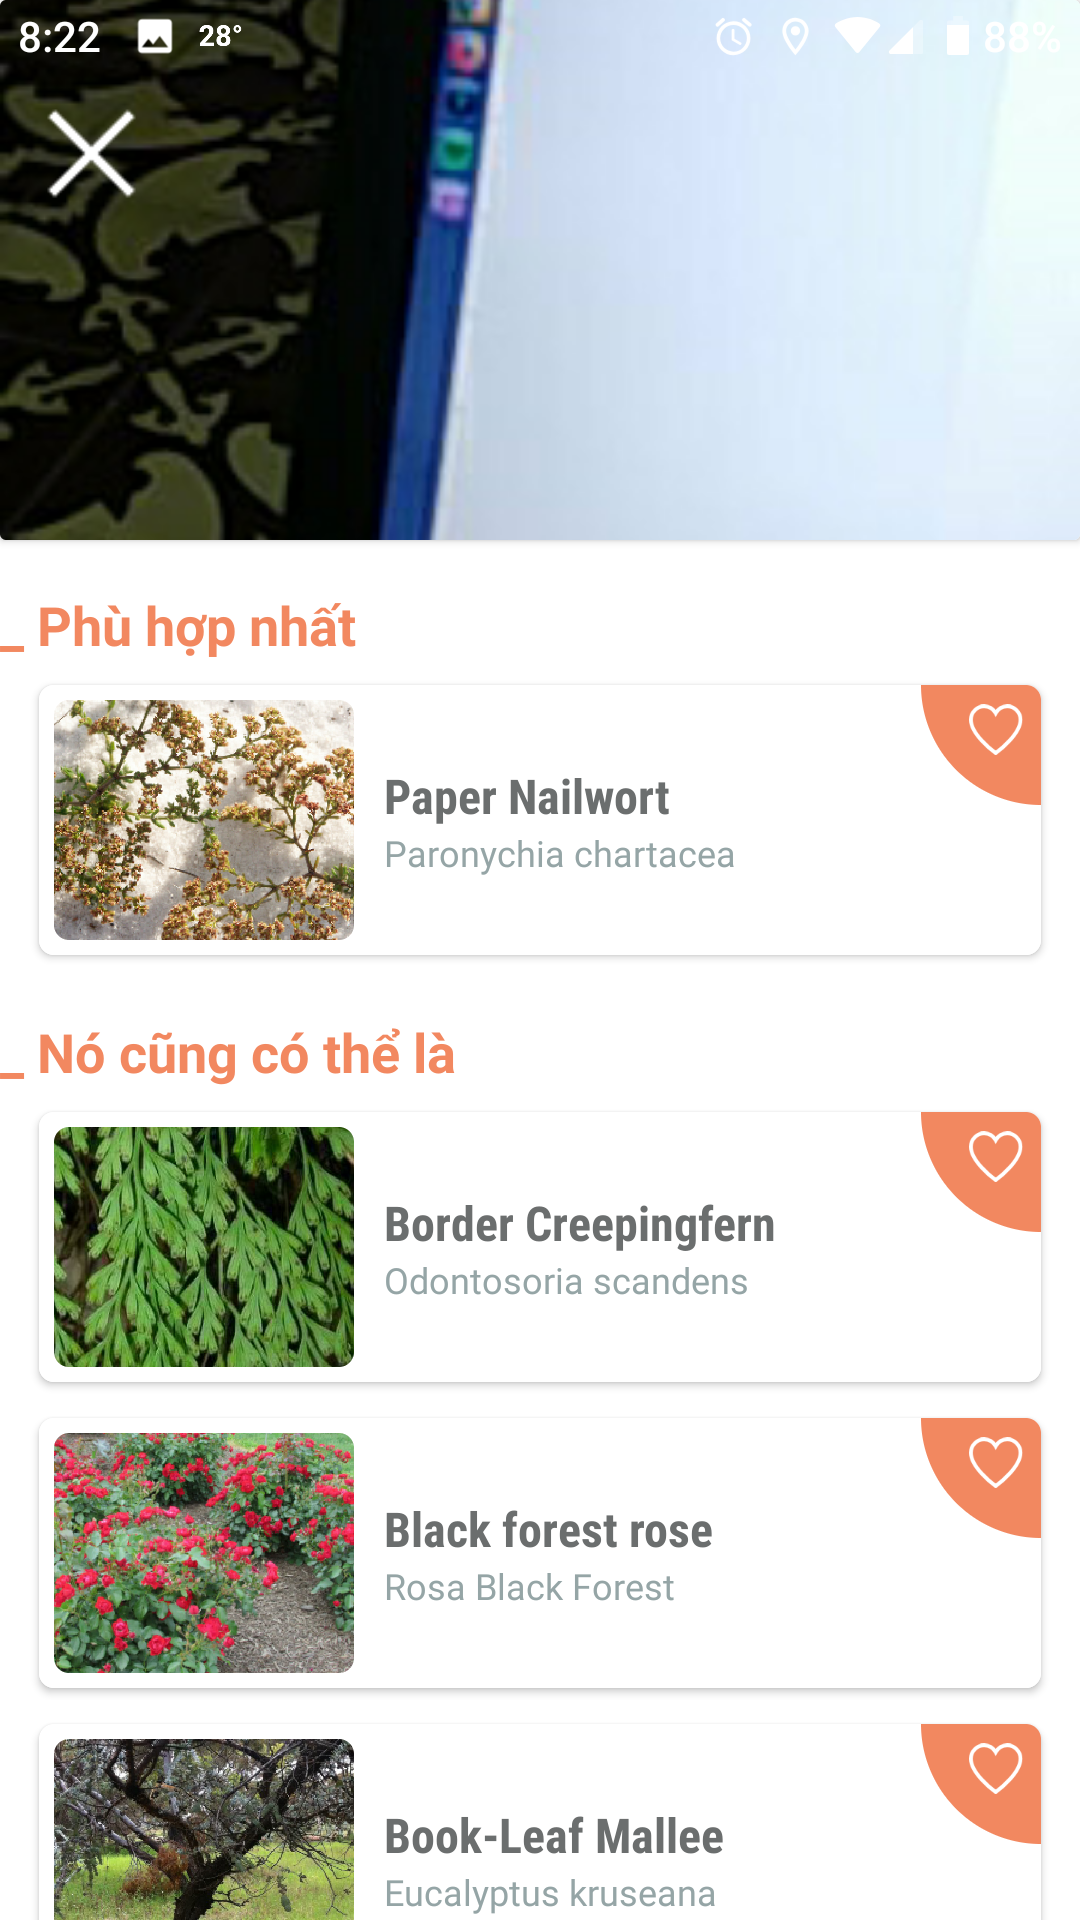
\includegraphics[scale=0.13]{app_detect1}
			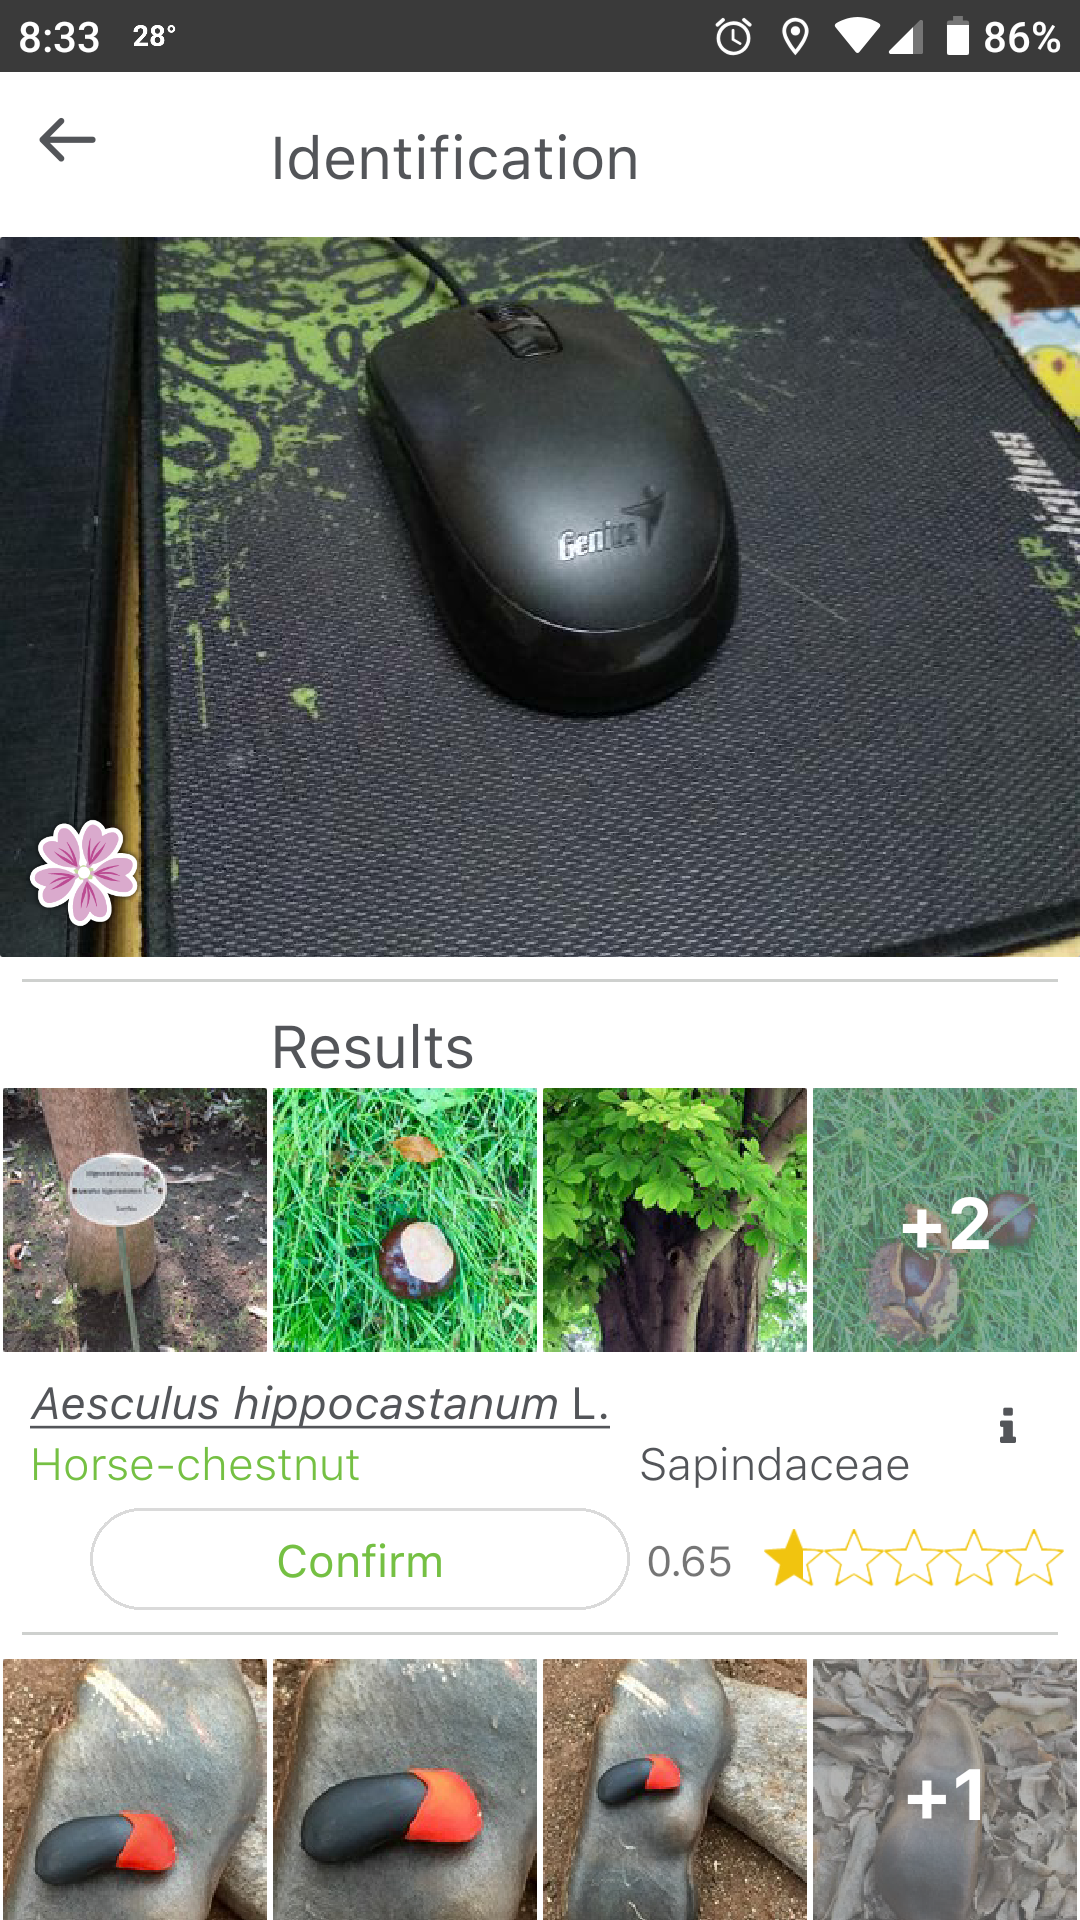
\includegraphics[scale=0.13]{app_detect2}
			\caption{Hình ảnh về ứng dụng chưa có chức năng phát hiện hoa trong ảnh}
			\label{fig:app_detect}
		\end{figure}
														
																
		% chương 3
		\newpage
		\chapter{Phát triển phần mềm nhận dạng hoa trên thiết bị di động}
		\label{chap:solution}
												
		Như đã trình bày tại chương 2, bước trích xuất thông tin từ ảnh là bước rất quan trọng trong mô hình nhận diện ảnh làm tốt bước này ta sẽ cải thiện được đáng kể độ chính xác và hiện nay có rất nhiều phương pháp để trích xuất thông tin từ ảnh. Để tăng cường độ chính xác nhận diện ảnh cho ứng dụng tôi có thêm một bước vào trước bước phân loại hoa đó là phát hiện ảnh có hoa hay không. 
												
		Để có thể làm tốt bước phát hiện hoa ta cần phải trích xuất được thuộc tính của cả các hình ảnh mà không có hoa trong đó, các hình ảnh không có hoa trong đó có thể thuộc rất nhiều các chủ đề như phong cảnh, động vật, đường phố .... Trong nghiên cứu [4] được công bố năm 2014 các tác giả đã đề xuất sử dụng mạng tích chập đã được huấn luyện bởi 1.2 triệu hình ảnh được lấy từ bộ dữ liệu ImageNet các hình ảnh thuộc rất nhiều chủ đề. Và kết quả thu được khi sử dụng một mô hình trích xuất nhưng lại có thể đáp ứng cho nhiều chủ đề ảnh khác nhau và thu được kết quả khá khả quan đối với chính bộ dữ liệu Oxford-102. 
												
		Theo nghiên cứu [16] cũng sử dụng mạng tích chập nhưng với mô hình có độ sâu các tầng tích chập lớn hơn thì sẽ cho được kết quả khả quan hơn. Vì vậy tôi đề xuất sử dụng mô hình mạng tích chập VGG19 [16] đã được xây dựng sẵn để làm bước trích xuất thông tin cho tất cả các bước trích xuất thông tin trong mô hình hệ thống.
												
		\section{Mô tả bài toán}
		Ứng dụng nhận dạng hoa trong khóa luận này sẽ có chức năng chính đó là nhận dạng hoa thông qua ảnh chụp. Như vậy đầu vào và đầu ra của bài toán sẽ là một hình ảnh được ghi lại từ các thiết bị ghi hình và đầu ra có thể có hai trường hợp																																																																			
																	
		\begin{itemize}
			\item \texttt{Trường hợp 1:} Trong ảnh không có hoa thì kết quả trả về là không tồn tại hoa.
			\item \texttt{Trường hợp 2:} Trong ảnh có hoa thì kết quả trả về là một danh sách 5 loài hoa có kết quả nhận dạng tốt nhất.
		\end{itemize}
		\begin{figure}[h]
			\centering
			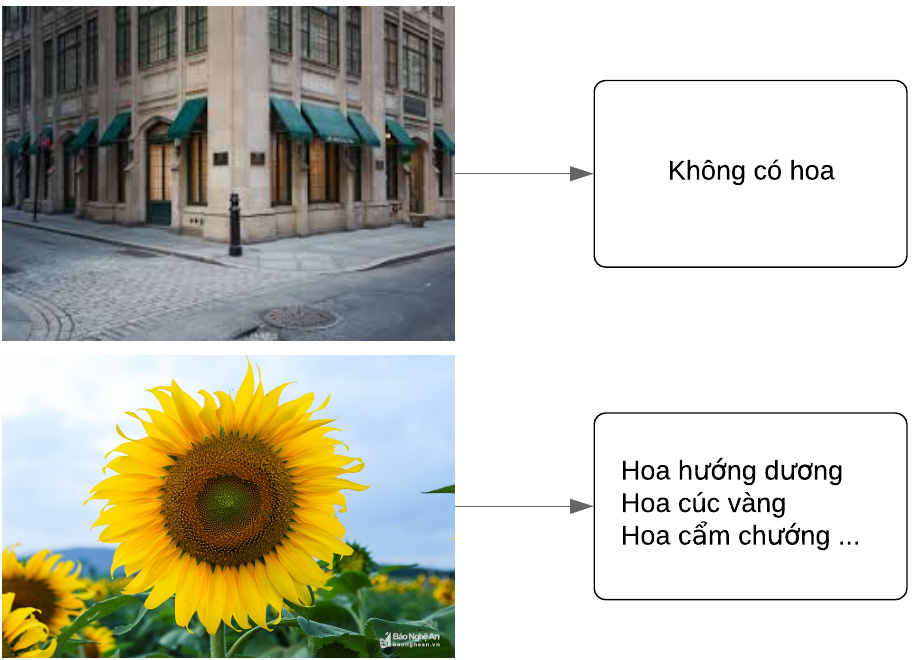
\includegraphics[scale=0.4]{mota_baitoan}
			\caption{Ví dụ về đầu vào và đầu ra của bài toán}
			\label{fig:mota_baitoan}
		\end{figure}
										
		\section{Mô tả mô hình hệ thống}
		Dưới đây là mô tả và giải thích chi tiết về các bước trong mô hình hệ thống qua sự tham khảo các nghiên cứu [1] [2] [3] [4] [16] và học hỏi về điểm mạnh và điểm yếu của các ứng dụng đã có về nhận dạng hoa trên thiết bị di động.
										
		\subsection{Mô hình chung}
		\begin{figure}[h]
			\centering
			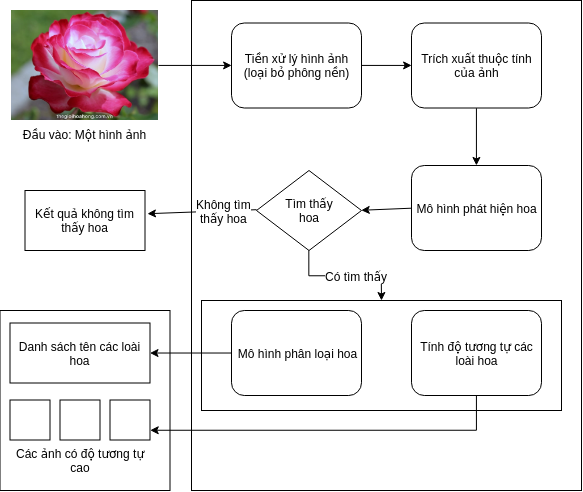
\includegraphics[scale=0.81]{mohinhchung}
			\caption{mô hình chung của hệ thống}
			\label{fig:mohinhchung}
		\end{figure}
										
		\textbf{Bước 1: Tiền xử lý dữ liệu.} 
		\begin{itemize}
			\item Do các ảnh của người dùng tải lên hệ thống có thể gặp phải một số trường hợp đặc biệt ví dụ như ảnh chụp bông hoa quá nhỏ, ảnh của hoa không nằm trong chính giữa bức ảnh ... Vì vậy, ảnh sau khi được chụp và gửi lên hệ thống sẽ được tiền xử lý bằng phương pháp tách phông nền để loại bỏ các phần không quan trọng.
			\item \texttt{Đầu vào:} Ảnh do người dùng chụp gửi lên hệ thống
			\item \texttt{Đầu ra:} Ảnh đã được tách phông nền.
		\end{itemize}
										
		\begin{figure}[h]
			\centering
			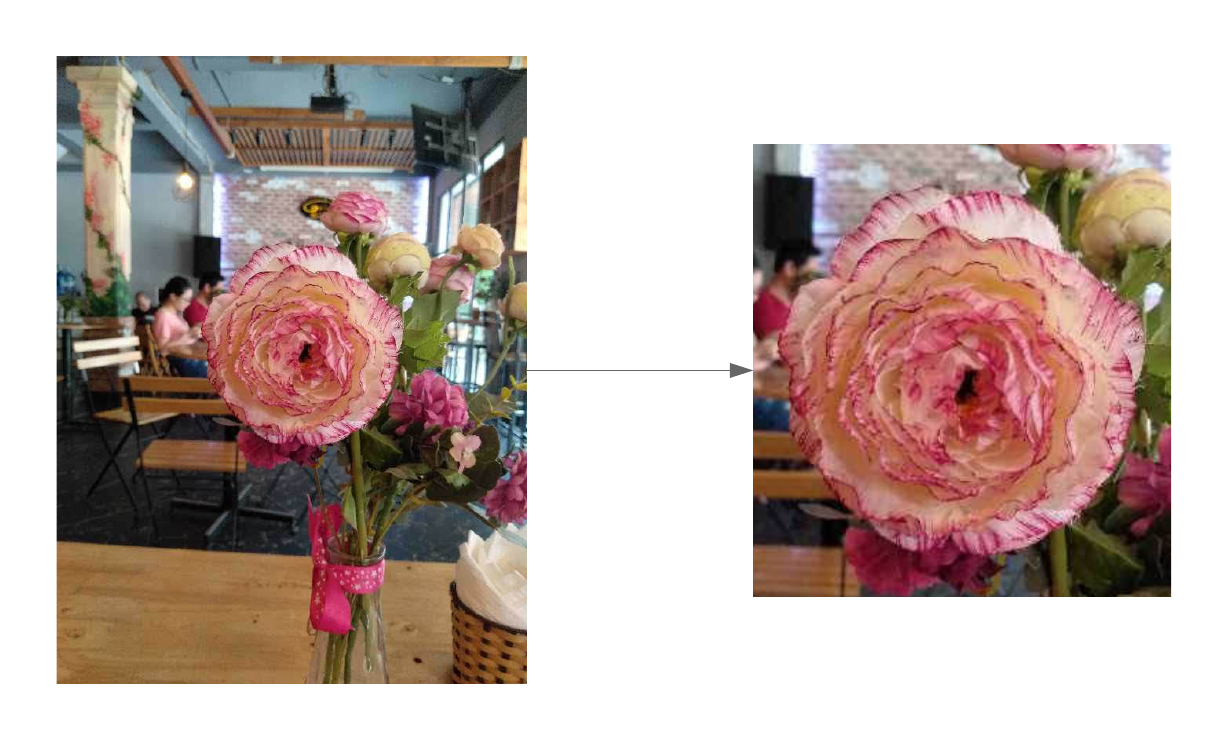
\includegraphics[scale=0.4]{tach_phong_nen}
			\caption{ví dụ về bước tách phông nền}
			\label{fig:tach_phong_nen}
		\end{figure}
										
		\textbf{Bước 2: Trích xuất thuộc tính.} 
		\begin{itemize}
			\item Đầu vào của bước này đó là bức ảnh mới có trọng tâm là chủ thể cần nhận dạng.
			\item Ảnh sẽ được thay đổi kích cỡ về dạng 224 x 224.
			\item Sử dụng mô hình VGG19 [16] để làm bước trích xuất thuộc tính. Dựa trên các cài đặt của mô hình VGG19 [16] ta đã nói ở phần 2.2.3 trong chương 2. Chỉ sử dụng đến tầng thứ 19 FC-4096 của mô hình và kết quả thu được ở đây là một vector thuộc tính có 4096 chiều.
			\item Vector thuộc tính sẽ được chuẩn hóa sẽ được chuẩn hóa L2 (L2 normalization).
		\end{itemize}
										
										
		\begin{lstlisting}
		from keras.applications.vgg19 import VGG19
		from keras.preprocessing import image
		from keras.applications.vgg19 import preprocess_input

		base_model = VGG19(weights='imagenet')
		model = Model(inputs=base_model.input,   outputs=base_model.get_layer('fc2').output)
		def get_feature_1_image(image_name):
			img_path = './' + image_name + '.jpg'
			img = image.load_img(img_path, target_size=(224, 224))
			x = image.img_to_array(img)
			x = np.expand_dims(x, axis=0)
			x = preprocess_input(x)
			features = model.predict(x)
		\end{lstlisting}
								
		\textbf{Bước 3: Phát hiện hoa trong ảnh.} 
		\begin{itemize}
			\item Sử dụng phương pháp máy vector hỗ trợ để xây dựng mô hình phân loại nhị phân (binary classification).
			\item Đầu vào của bước này là vector thuộc tính đã được sinh ra ở bước 2.
			\item Nếu kết quả của mô hình phát hiện ảnh là không có hoa thì lập tức trả lại kết quả cho người dùng là không tìm thấy hoa.
			\item Nếu kết quả là có hoa thì chuyển vector thuộc tính sang bước 4.
		\end{itemize}
										
										
		\textbf{Bước 4: Phân loại hoa.} 
		\begin{itemize}
			\item Sử dụng phương pháp máy vector hỗ trợ để xây dựng mô hình phân loại chi tiết về cách xây dựng mô hình sẽ được nói kỹ hơn ở phần sau của chương.
			\item Đầu vào của bước này là vector thuộc tính đã qua bước phát hiện hoa.
			\item Kết quả của mô hình phân loại ở bước này sẽ cho ta danh sách tên các loài hoa theo thứ tự là có độ phù hợp cao nhất đến thấp nhất. Trong ứng dụng này sẽ lấy ra tên 5 loài hoa có độ phù hợp cao nhất.
		\end{itemize}
										
		Như đã có ở bước thứ 4, kết quả đi ra sẽ là danh sách tên 5 loài hoa. Ở đây, nếu nhiệm vụ của bài toán chỉ là cho ra tên của loài hoa thì có vẻ như không cần bước này. Trong thực tế một loài hoa hồng như có thể xuất hiện trong tự nhiên với khá nhiều màu sắc như hoa hồng đỏ, hoa hồng trắng, vàng. Vì vậy khi tìm kiếm một bông hồng trắng nếu ta sẽ đưa ra danh sách tên của loài hoa đó và kèm theo đó là một bức ảnh có độ tương tự gần giống nhất với bức ảnh cần tìm kiếm của mỗi loài.
								
		\textbf{Bước 5: Tính độ tương tự của các loài.} 
		\begin{itemize}
			\item Độ tương tự được tính ở đây là cosin giữa hai vector.
			      Ở trên đây là công thức tính độ tương tự giữa góc giữa hai hình ảnh A và B trong đó A và B lần lượt là các vector thuộc tính của 2 hình ảnh A và B. 
			      			      			      			
			      ||A|| là độ dài của vector thuộc tính A\\
			      ||B|| là độ dài vector thuộc tính B\\
			      Độ tương tự sẽ lớn nhất khi vector A trùng vector B và công thức trên cho kết quả bằng 1.
			      \begin{figure}[h]
			      	\centering
			      	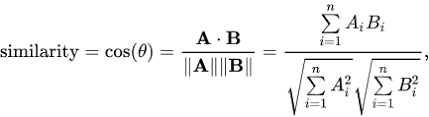
\includegraphics[scale=0.8]{cosin}
			      \end{figure}
			\item Trong mỗi loài hoa được nhận ra ảnh nào có độ tương tự lớn nhất với ảnh cần tìm thì ta sẽ hiển thị ra ảnh đó, để người dùng có thể dễ dàng xác nhận được đúng loài hoa cần tìm.
		\end{itemize}	
										
		\subsection{Mô hình phát hiện hoa}
		\begin{figure}[h]
			\centering
			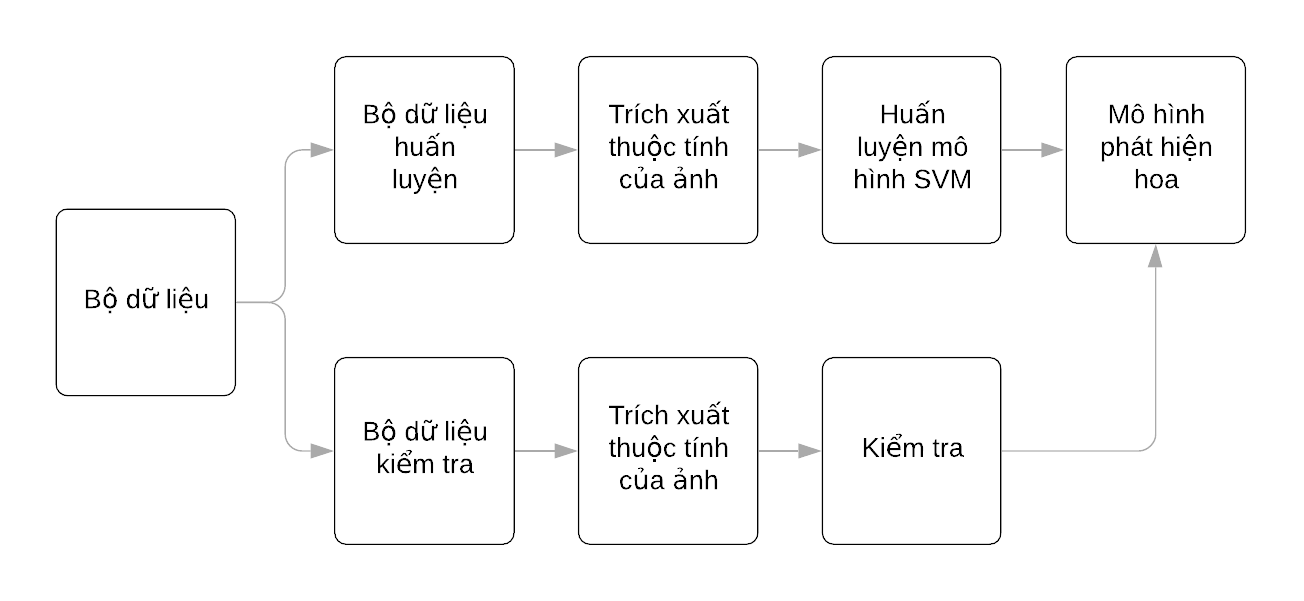
\includegraphics[scale=0.4]{mohinh_phathien}
			\caption{Mô hình phát hiện hoa}
			\label{fig:mohinh_phathien}
		\end{figure}
						
		\textbf{Bước 1: Chuẩn bị dữ liệu.} 
		\begin{itemize}
			\item Bộ dữ liệu bao gồm 10.290 ảnh trong đó có 5132 ảnh có hoa và 5158 ảnh được thu thập từ bộ dữ liệu ImageNet.
			\item Chia bộ dữ liệu thành các tập con.
			      \begin{itemize}
			      	\item \texttt{Bộ dữ liệu kiểm tra :} 1000 ảnh (mỗi lớp có 500 ảnh).
			      	\item \texttt{Bộ dữ liệu xác nhận :} 1000 ảnh (mỗi lớp có 500 ảnh).
			      	\item \texttt{Bộ dữ liệu huấn luyện:} các ảnh còn lại (cụ thể 4132 ảnh có hoa và 4158 ảnh không có hoa).
			      \end{itemize}
		\end{itemize}
										
		\textbf{Bước 2: Trích xuất thuộc tính.} 
		\begin{itemize}
			\item Ảnh sẽ được thay đổi kích cỡ về dạng 224 x 224.
			\item Sử dụng mô hình VGG19 [16] để làm bước trích xuất thuộc tính. Dựa trên các cài đặt của mô hình VGG19 [16] ta đã nói ở phần 2.2.3 trong chương 2. Chỉ sử dụng đến tầng thứ 19 FC-4096 của mô hình và kết quả thu được ở đây là một vector thuộc tính có 4096 chiều.
			\item Vector thuộc tính sẽ được chuẩn hóa sẽ được chuẩn hóa L2 (L2 normalization).
		\end{itemize}
						
		\textbf{Bước 3: Huấn luyện mô hình.} 
		\begin{itemize}
			\item Sử dụng phương pháp máy vector hỗ trợ để xây dựng mô hình phân loại nhị phân (binary classification). 
			\item Lấy bộ dữ liệu huấn luyện để huấn luyện cho mô hình, và sử dụng bộ xác nhận để đo độ chính xác của mô hình.
			\item kết quả thu được là mô hình phát hiện hoa.
			      			      			      
		\end{itemize}
						
		\textbf{Bước 4: Kiểm tra mô hình.} 
		\begin{itemize}
			\item Sử dụng bộ kiểm tra để đo độ chính xác của mô hình vừa nhận được.
		\end{itemize}
						
						
		\newpage
		\subsection{Mô hình phân loại hoa}
		\begin{figure}[h]
			\centering
			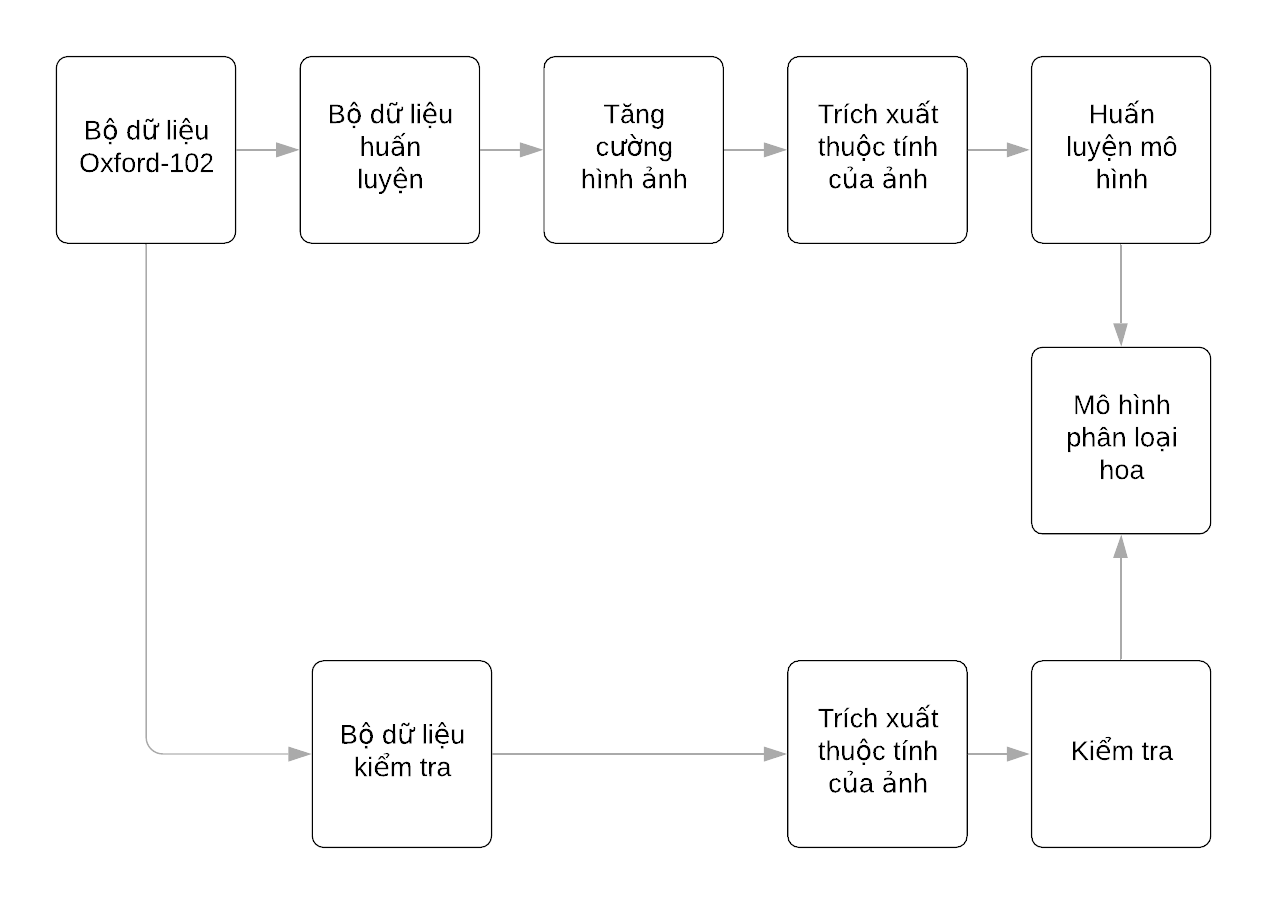
\includegraphics[scale=0.4]{mohinh_phanloai}
			\caption{Mô hình phân loại hoa}
			\label{fig:mohinh_phanloai}
		\end{figure}
						
		\textbf{Bước 1: Chuẩn bị dữ liệu.} 
		\begin{itemize}
			\item Ở đây sử dụng bộ dữ liệu Oxford-102 [1], nhận thấy số lượng ảnh để huấn luyện cho mô hình chỉ là 10 ảnh mỗi loài hoa, như vậy là hơi ít ảnh vì vậy tôi đã gộp bộ huấn luyện và bộ xác nhận lại thành bộ huấn luyện mở rộng. Sau đó sử dụng phương pháp tăng cường ảnh [17] để tăng số lượng ảnh huấn luyện.
			\item Do bộ dữ liệu chia lượng ảnh huấn luyện ít mà ảnh dùng để kiểm tra lại nhiều nên tôi đã chia bộ dữ liệu theo cách mới đó là cắt một nửa bộ kiểm tra (mỗi loài hoa trong tập kiểm tra chia một nửa cho bộ huấn luyện nửa còn lại để kiểm tra).
			\item Các ảnh trong bộ dữ liệu đều là ảnh chụp cận cảnh bông hoa vì vậy ở mô hình này không cần đến bước tách phông nền.
		\end{itemize}
						
		\textbf{Bước 2: Trích xuất thuộc tính.} 
		\begin{itemize}
			\item Đầu vào của bước này đó là bức ảnh mới có trọng tâm là chủ thể cần nhận dạng.
			\item Ảnh sẽ được thay đổi kích cỡ về dạng 224 x 224.
			\item Sử dụng mô hình VGG19 [16] để làm bước trích xuất thuộc tính. Dựa trên các cài đặt của mô hình VGG19 [16] ta đã nói ở phần 2.2.3 trong chương 2. Chỉ sử dụng đến tầng thứ 19 FC-4096 của mô hình và kết quả thu được ở đây là một vector thuộc tính có 4096 chiều.
			\item Vector thuộc tính sẽ được chuẩn hóa sẽ được chuẩn hóa L2 (L2 normalization).
		\end{itemize}
						
		\textbf{Bước 3: Huấn luyện mô hình.} 
		\begin{itemize}
			\item Sử dụng phương pháp máy vector hỗ trợ để xây dựng mô hình phân loại.
			\item Lấy bộ dữ liệu huấn luyện để huấn luyện cho mô hình. Kết quả thu được là mô hình phát hiện hoa.
		\end{itemize}
						
		\textbf{Bước 4: Kiểm tra mô hình.} 
		\begin{itemize}
			\item Sử dụng bộ kiểm tra để đo độ chính xác của mô hình vừa nhận được.
		\end{itemize}
							
		% chương 4				
		\chapter{Kết quả thực nghiệm}
		\label{chap:Experimental results}
		Tại chương 4 này sẽ nói về cách thu thập các bộ dữ liệu, triển khai cài đặt các phần của ứng dụng dựa trên các phương pháp giải quyết vấn đề đã đặt ra ở chương 3. Chúng ta có một ứng dụng nhận dạng các loài hoa sử dụng thư viện React Native viết cho cả hai hệ điều hành là android và IOS. Ứng dụng sẽ truyền và nhận dữ liệu từ một máy chủ sử dụng các mô hình phân loại đã được huấn luyện. Đồng thời trong chương này cũng công bố các kết quả về các mô hình phân loại đã đạt được
						
		\section{Xây dựng bộ dữ liệu.}
		\subsection{Bộ dữ liệu dùng để phát hiện đối tượng hoa trong ảnh.}
						
		\textbf{Cách thu thập:} Sử dụng bộ dữ liệu ImageNet tại trang web : http://www.image-net.org để thu thập các ảnh. Các ảnh tại đây đã được chia sẵn thành các chủ đề nhỏ, đa dạng về chủ đề. Tổng cộng là 5158 ảnh không có hoa. Để lấy các bức ảnh không có hoa là chủ thể chính trong ảnh tôi lựa chọn các chủ đề: 
		\begin{itemize}
			\item Động vật có vú		: bao gồm 743 ảnh.
			\item Cảnh vật trong tự nhiên	: bao gồm 930 ảnh.
			\item Đồ ăn			: bao gồm 1063 ảnh.
			\item Cảnh vật trong phòng	: bao gồm 659 ảnh.
			\item Công cụ máy móc		: bao gồm 799 ảnh.
			\item Đường phố			: bao gồm 964 ảnh.
		\end{itemize}	
							
				
		\begin{figure}[h]
			\centering
			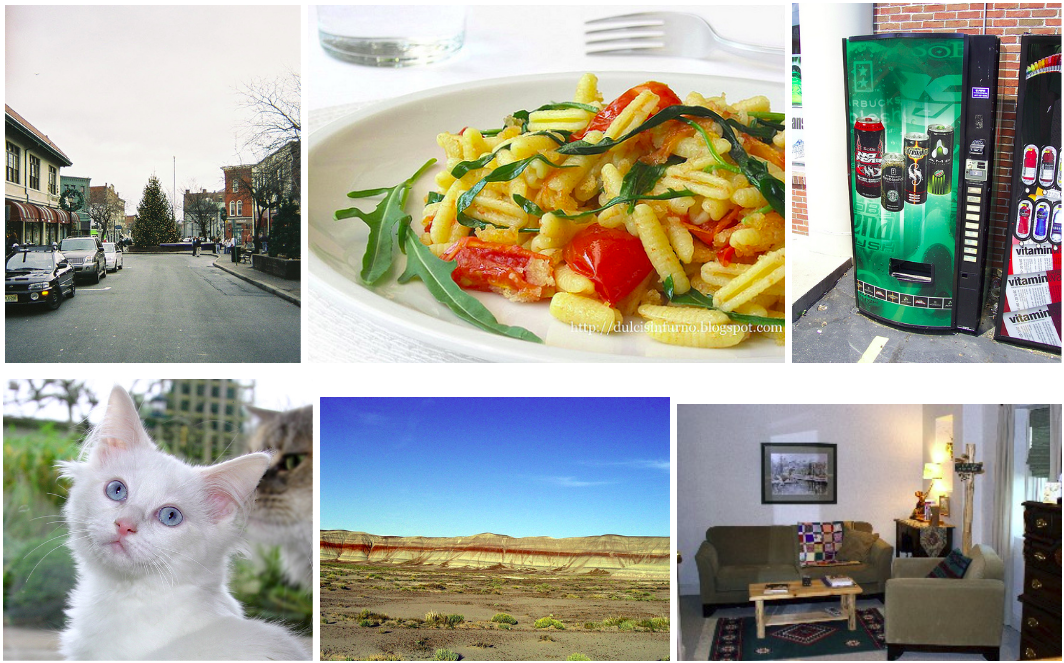
\includegraphics[scale=0.4]{nonflower}
			\caption{Hình ảnh lấy trong bộ ảnh không có hoa}
			\label{fig:nonflower}
		\end{figure}
				
		Bộ dữ liệu có hoa tôi lấy từ chủ đề "flower" thu thập được 1207 ảnh. Nhận thấy có sự chênh lệch khá lớn giữa bộ ảnh có hoa và không có hoa nên tôi sử dụng một phần bộ dữ liệu Oxford-102 [1], vào để số lượng ảnh có hoa và không có hoa mang tính cân đối. Tổng cộng là 5132 ảnh trong đó có:
		\begin{itemize}
			\item Ảnh có hoa từ ImageNet: bao gồm 1207 ảnh.
			\item Ảnh lấy từ Oxford-102	: bao gồm 3925 ảnh.
		\end{itemize}
				
		\begin{figure}[h]
			\centering
			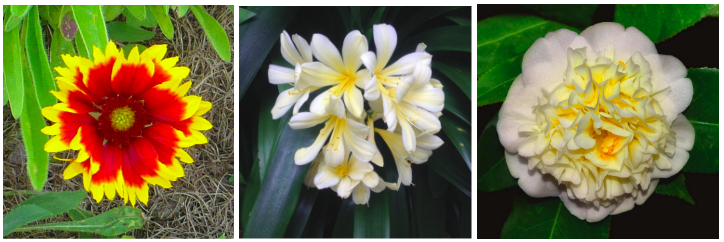
\includegraphics[scale=0.6]{anhcohoa}
			\caption{Hình ảnh lấy trong bộ ảnh có hoa}
			\label{fig:anhcohoa}
		\end{figure}
				
		\textbf{Cách chia bộ dữ liệu:} Bộ dữ liệu được chia thành 3 tập
		\begin{itemize}
			\item \texttt{Tập dữ liệu kiểm tra} gồm 1000 ảnh (500 ảnh có hoa và 500 ảnh không có hoa).
			\item \texttt{Tập dữ liệu xác nhận} gồm 1000 ảnh (500 ảnh có hoa và 500 ảnh không có hoa).
			\item \texttt{Tập dữ liệu huấn luyện} gồm 8290 ảnh (4132 ảnh có hoa và 4158 ảnh không có hoa).
		\end{itemize}
				
				
		\textbf{Khó khăn và hạn chế:} Tại trang ImageNet các ảnh để dưới dạng đường link nên khi tôi lọc ảnh đã gặp phải khá nhiều khó khăn như sau.
		\begin{itemize}
			\item Ảnh bị lỗi không thể hiển thị (ví dụ là bộ dữ liệu động vật có vú theo như công bố trên trang web có 1169 ảnh nhưng thực tế khi thu thập chỉ còn 743 ảnh, hay như bộ ảnh hoa công bố là 1924 ảnh nhưng khi thu thập lại chỉ còn 1207 ảnh, các bộ dữ liệu khác cũng tương tự chỉ thu thập được tầm 50-80\% ảnh) Đường link không còn được sử dụng, đường link đến hệ thống nước ngoài nên thời gian phản hồi rất lâu
			\item Một số ảnh quá bé, quá nặng.
			\item Số ảnh tôi công bố dùng làm bộ dữ liệu ở trên là các ảnh đã bỏ đi các ảnh lỗi ảnh quá bé, quá nhỏ, …
			\item Các ảnh trong bộ ảnh không có hoa đôi khi vẫn còn sót lại vài ảnh có xuất hiện bông hoa khá to trong đó. Tương tự như vậy, trong bộ ảnh có hoa lấy từ ImageNet vẫn còn có vài ảnh chỉ có chụp thân hoặc gốc cây tỷ lệ này được ghi nhận ở dưới mức 3\%. Tôi đã ngồi duyệt lại bằng tay để lọc ra các ảnh đặc biệt.
		\end{itemize}
				
					
		\subsection{Bộ dữ liệu dùng để phân loại tên loài hoa}
						
		\textbf{Cách thu thập:} Tôi tải về bộ dữ liệu Oxford-102 [1], tại trang web của trường đại học Oxford. Tại bộ dữ liệu có các tập tin đi kèm.
		\begin{itemize}
			\item \texttt{imagelabel.mat:} chứa danh sách tên các loài hoa ứng với từng bức ảnh theo dạng số từ 1 tới 102.
			\item \texttt{setid.mat:} chứa cách phân chia bộ dữ liệu ra thành 3 tập dữ liệu nhỏ đó là bộ huấn luyện, bộ xác nhận và bộ kiểm tra.
		\end{itemize}
				
		\textbf{Chuyển đổi bộ dữ liệu sang tiếng việt.}
		Tại tập tin "imagelabel.mat" của bộ dữ liệu chỉ có tên loài hoa đánh dưới dạng số. Ví dụ trong đó là số 74 tương ứng với loài hoa hồng.
				
		\begin{figure}[h]
			\centering
			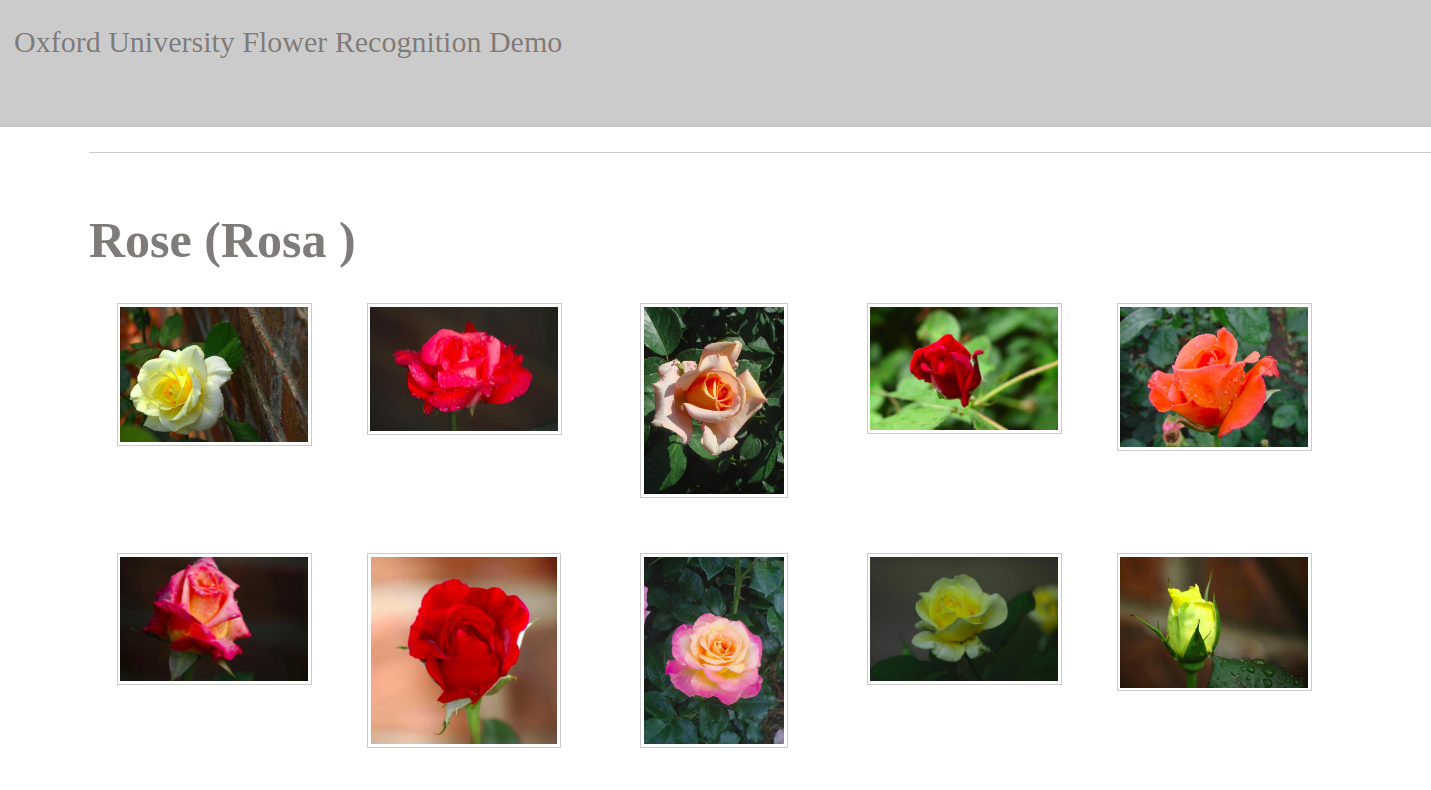
\includegraphics[scale=0.35]{rose_oxford}
			\caption{Hình ảnh về trang web chứa tên loài hoa của bộ dữ liệu Oxford-102}
			\label{fig:rose_oxford}
		\end{figure}
				
		Có thể thấy tiêu đề của trang "Rose (Rosa)" được viết dưới dạng "Tên tiếng Anh( Tên Latin)". Tôi sử dụng công cụ Scrapy dành cho ngôn ngữ python để trích xuất tự động danh sách tên của các loài hoa từ 1 đến 102 vào một file văn bản. Sau đó sử dụng Google và Wikipedia để tra cứu tên tiếng Anh hoặc tên Latin để tìm kiếm ra tên tiếng việt và đặc điểm cũng như cách trồng của từng loại hoa từ đó thêm vào cơ sở dữ liệu.
						
		Trong lúc tìm tên tiếng việt cho các loài hoa tôi gặp phải một số những khó khăn sau:
		\begin{itemize}
			\item Bộ dữ liệu Oxford-102 [1], này bao gồm các loài hoa phổ biến có mọc tại Anh nên một số loài hoa chỉ có giải thích bằng tiếng Anh nên rất khó khăn trong giai đoạn tìm tên, đặc điểm sinh trưởng cũng như cách trồng.
			\item Khi tìm kiếm trên Google về cách trồng và đặc điểm sinh trưởng tôi phải tìm ở rất nhiều trang web có những cấu trúc HTML rất khác nhau vì vậy công việc này hiện tôi phải làm thủ công bằng tay để có thể tìm được thông tin chi tiết về 102 loài hoa.
		\end{itemize}
				
		\subsection{Bộ dữ liệu ảnh chụp thực tế.}
		\textbf{Cách thu thập.}
				
		Mục tiêu của bộ dữ liệu này là dùng để kiểm tra mô hình phân loại. Vì ứng dụng của tôi muốn hướng tới là một ứng dụng nhận dạng hoa dành cho người Việt vì vậy các loài hoa mọi người thường hay tìm kiếm sẽ là các loài hoa phổ biến được trồng và mọc tại Việt Nam. Tôi lựa chọn ở đây gồm có 18 loài hoa phổ biến mọc tại Việt Nam các ảnh ở đây là một phần là do chính tôi chụp bằng điện thoại di động, một phần lấy từ trang diễn đàn vnphoto.net và google images. Số lượng ảnh mỗi loài hoa là 40 ảnh mỗi loại vì một loài hoa có thể có nhiều màu ví dụ như hoa giấy có màu tím, hồng và trắng thì số lượng mỗi màu sắc của mỗi loài sẽ gần bằng nhau. Tổng cộng tôi thu thập 720 ảnh của 18 loài hoa danh sách cụ thể các loài hoa và số lượng màu sắc tôi để trong bảng dưới đây.
				
				
		\begin{table}[h]
			\centering
			\caption{Bảng danh sách các loài hoa phổ biến ở Việt Nam có trong bộ dữ liệu ảnh chụp thực tế}
			\label{tbl:table ket qua cua Nilsback08}
			\begin{tabular}{|l|l|}
				\hline
				Hoa bìm bìm (hồng, tím)               & Hoa giấy (tím, hồng, trắng) \\ \hline
				Hoa cẩm chướng (đỏ, vàng, hồng) & Hoa hồng (đỏ, hồng, vàng)  \\ \hline
				Hoa cúc (cam, vàng, tím)                & Hoa hướng dương        \\ \hline       
				Hoa cúc vạn thọ                       & Hoa ly (cam, vàng)           \\ \hline     
				Hoa đại                                 & Hoa mộc lan               \\ \hline       
				Hoa dâm bụt (đỏ, hồng, vàng)      & Hoa păng xê                     \\ \hline 
				Hoa đỗ quyên                         & Hoa sen                      \\ \hline      
				Hoa trạng nguyên (đỏ, trắng)       & Hoa súng (vàng, trắng)         \\ \hline
				Hoa trà (trắng hồng)                  & Hoa thiên điểu              \\ \hline   			
			\end{tabular}
		\end{table}

		\section{Môi trường thực nghiệm}
		Cấu hình phần cứng:
		\begin{itemize}
			\item CPU	: Intel core i5-4200H - 2.8Ghz x 4
			\item RAM	: 8GB
			\item OS	: Ubuntu 16.04 LTS - 64 bit
		\end{itemize}


		Các thư viện cần cài đặt trước khi tiến hành các thí nghiệm:

		\begin{itemize}
			\item Python 2, NodeJS, Java 8.
			\item Bộ thư viện sklearn trên python.
			\item Bộ thư viện keras trên python.
		\end{itemize}
		
		\section{Xây dựng và cài đặt ứng dụng trên thiết bị di động}
		Sử dụng bộ thư viện React Native để xây dựng ứng dụng di động native sử dụng Javascript do Facebook phát hành. Sử dụng React Native để chỉ cần viết một lần duy nhất có thể xây dựng được ứng dụng cho cả iOS và Android.
		\subsection{Mô tả sơ đồ các ca sử dụng chính của ứng dụng}
		
		\begin{figure}[h]
			\centering
			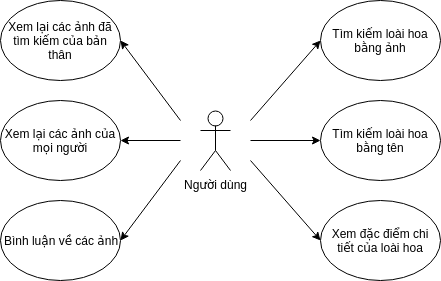
\includegraphics[scale=1]{usecase}
			\caption{Hình ảnh về các ca sử dụng của ứng dụng}
			\label{fig:usecase}
		\end{figure}
		Các ca sử dụng của ứng dụng là :

		\begin{itemize}
			\item Tìm kiếm, nhận dạng loài hoa bằng ảnh.
			\item Tìm kiếm loài hoa bằng tên.
			\item Xem đặc điểm chi tiết của loài hoa đó.
			\item Xem lại các ảnh của bản thân.
			\item Xem các ảnh của mọi người tải lên hệ thống.
			\item Bình luận và phản hồi về các ảnh.
		\end{itemize}

		\subsection{Giao diện của ứng dụng trên điện thoại di động}
		Ở giao diện tra cứu có các chức năng như là tìm kiếm trực tiếp bằng ảnh chụp hoặc tìm kiếm bằng tên loài hoa. Các chức năng cài đặt cho máy ảnh như tắt/bật đèn chớp, xoay máy ảnh ra phía trước, hoặc sử dụng ảnh có sẵn trong album để tìm kiếm.

		\begin{figure}[h]
			\centering
			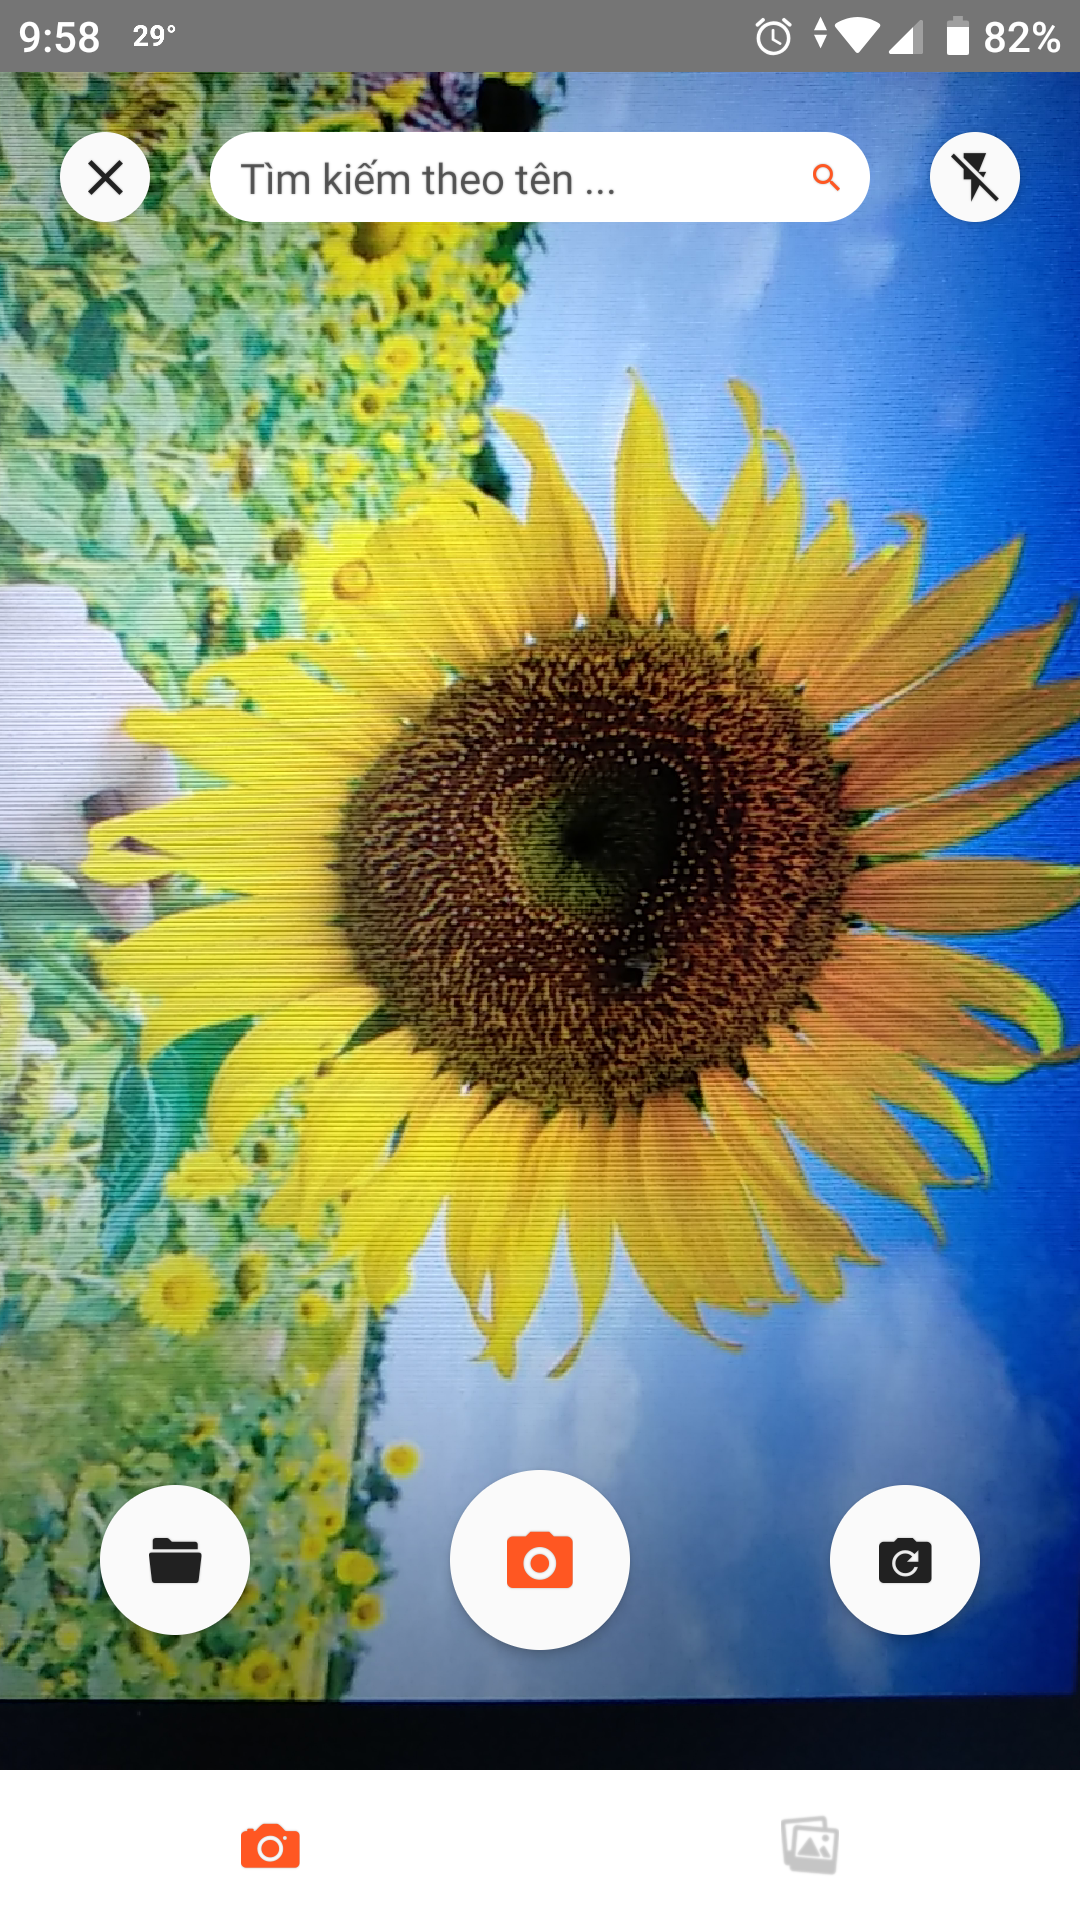
\includegraphics[scale=0.2]{app_search1}
			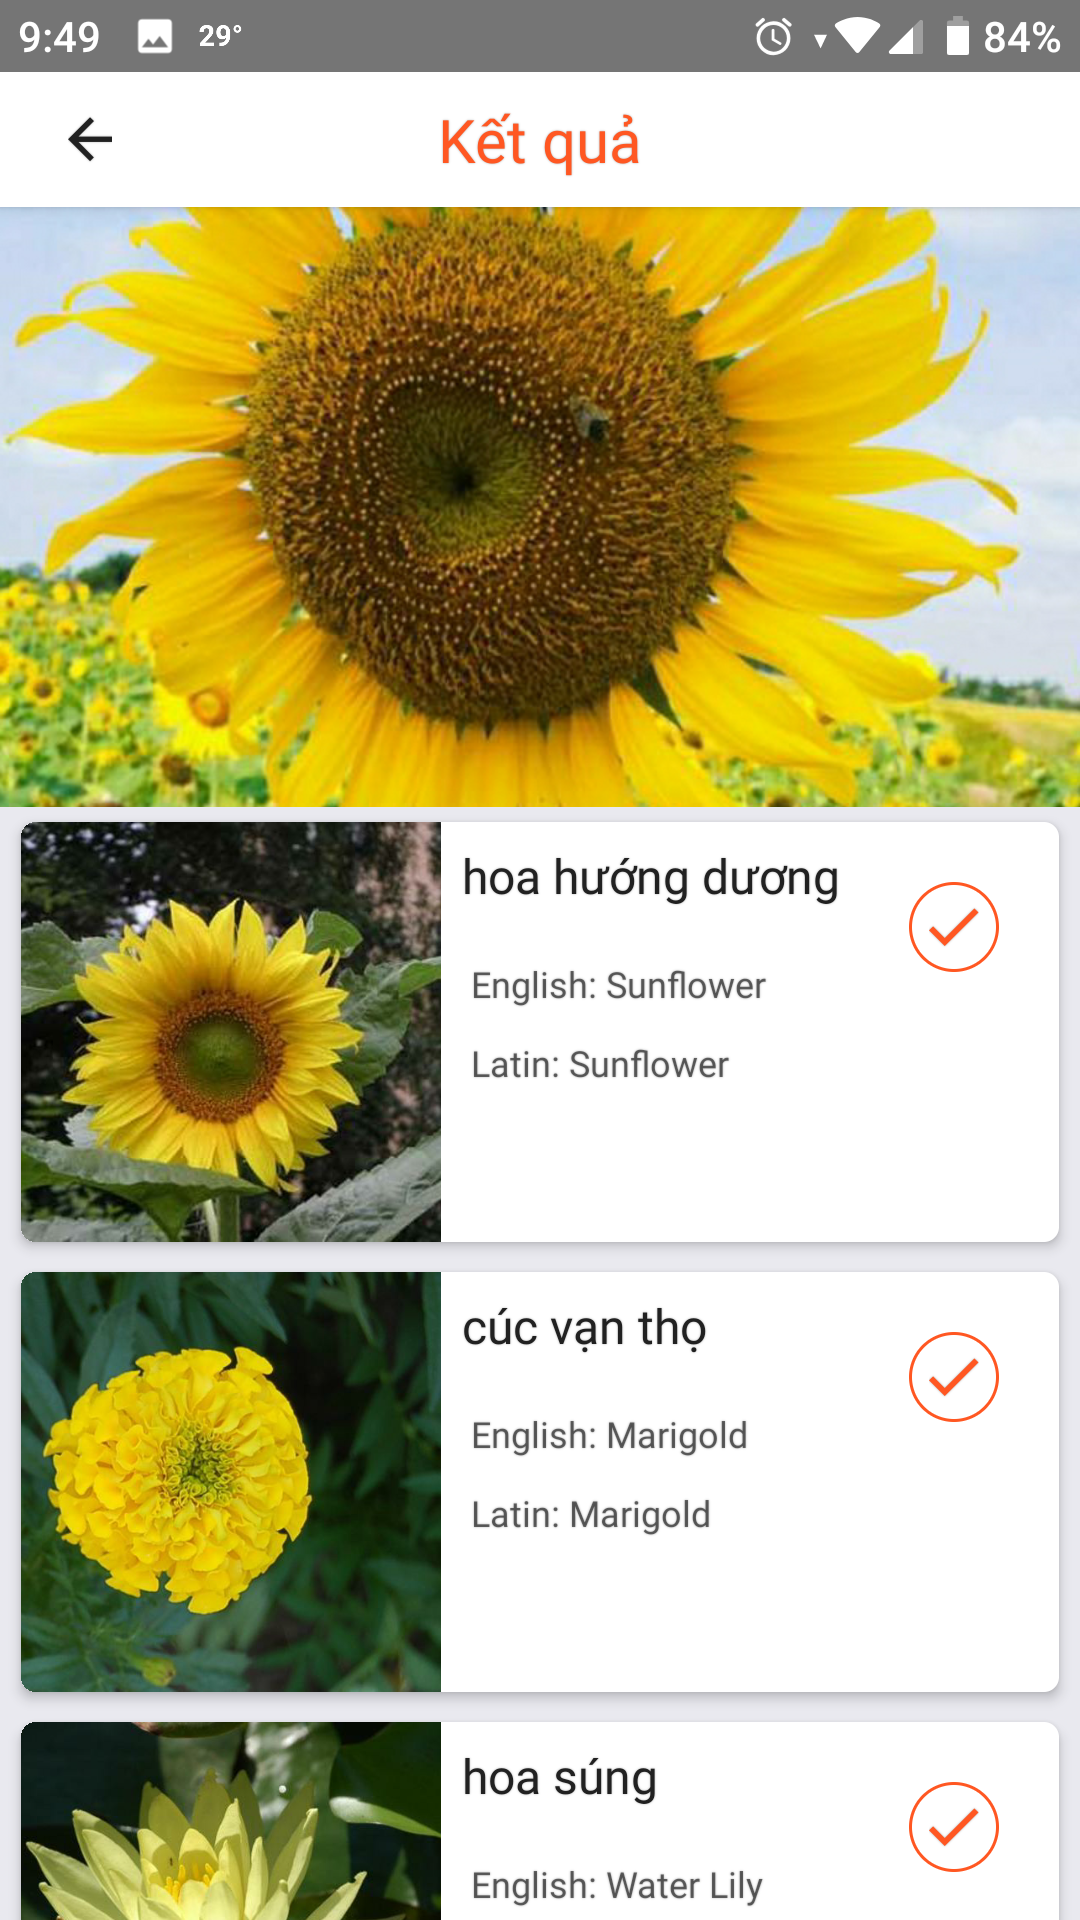
\includegraphics[scale=0.2]{app_search2}
			\caption{Hình ảnh giao diện tra cứu và kết quả tra cứu của ứng dụng.}
			\label{fig:app_search}
		\end{figure}

		Ở giao diện kết quả tìm kiếm bằng ảnh ta sẽ nhìn thấy danh sách các loài hoa phù hợp nhất với ảnh chụp đó. Các loài hoa sẽ được sắp xếp theo thứ tự từ trên xuống dưới tương ứng với mức độ phù hợp cao đến thấp. Danh sách tên các loài hoa hiển thị bao gồm tên tiếng Việt, tên tiếng Anh, tên tiếng Latin và đi kèm với đó là hình ảnh đại diện là hình ảnh của loài hoa trong cơ sở dữ liệu có độ tương tự cao nhất với ảnh tìm kiếm. Khi chụp một bức ảnh không có hoa thì kết quả trả về sẽ là không tìm thấy hoa.

		\begin{figure}[h]
			\centering
			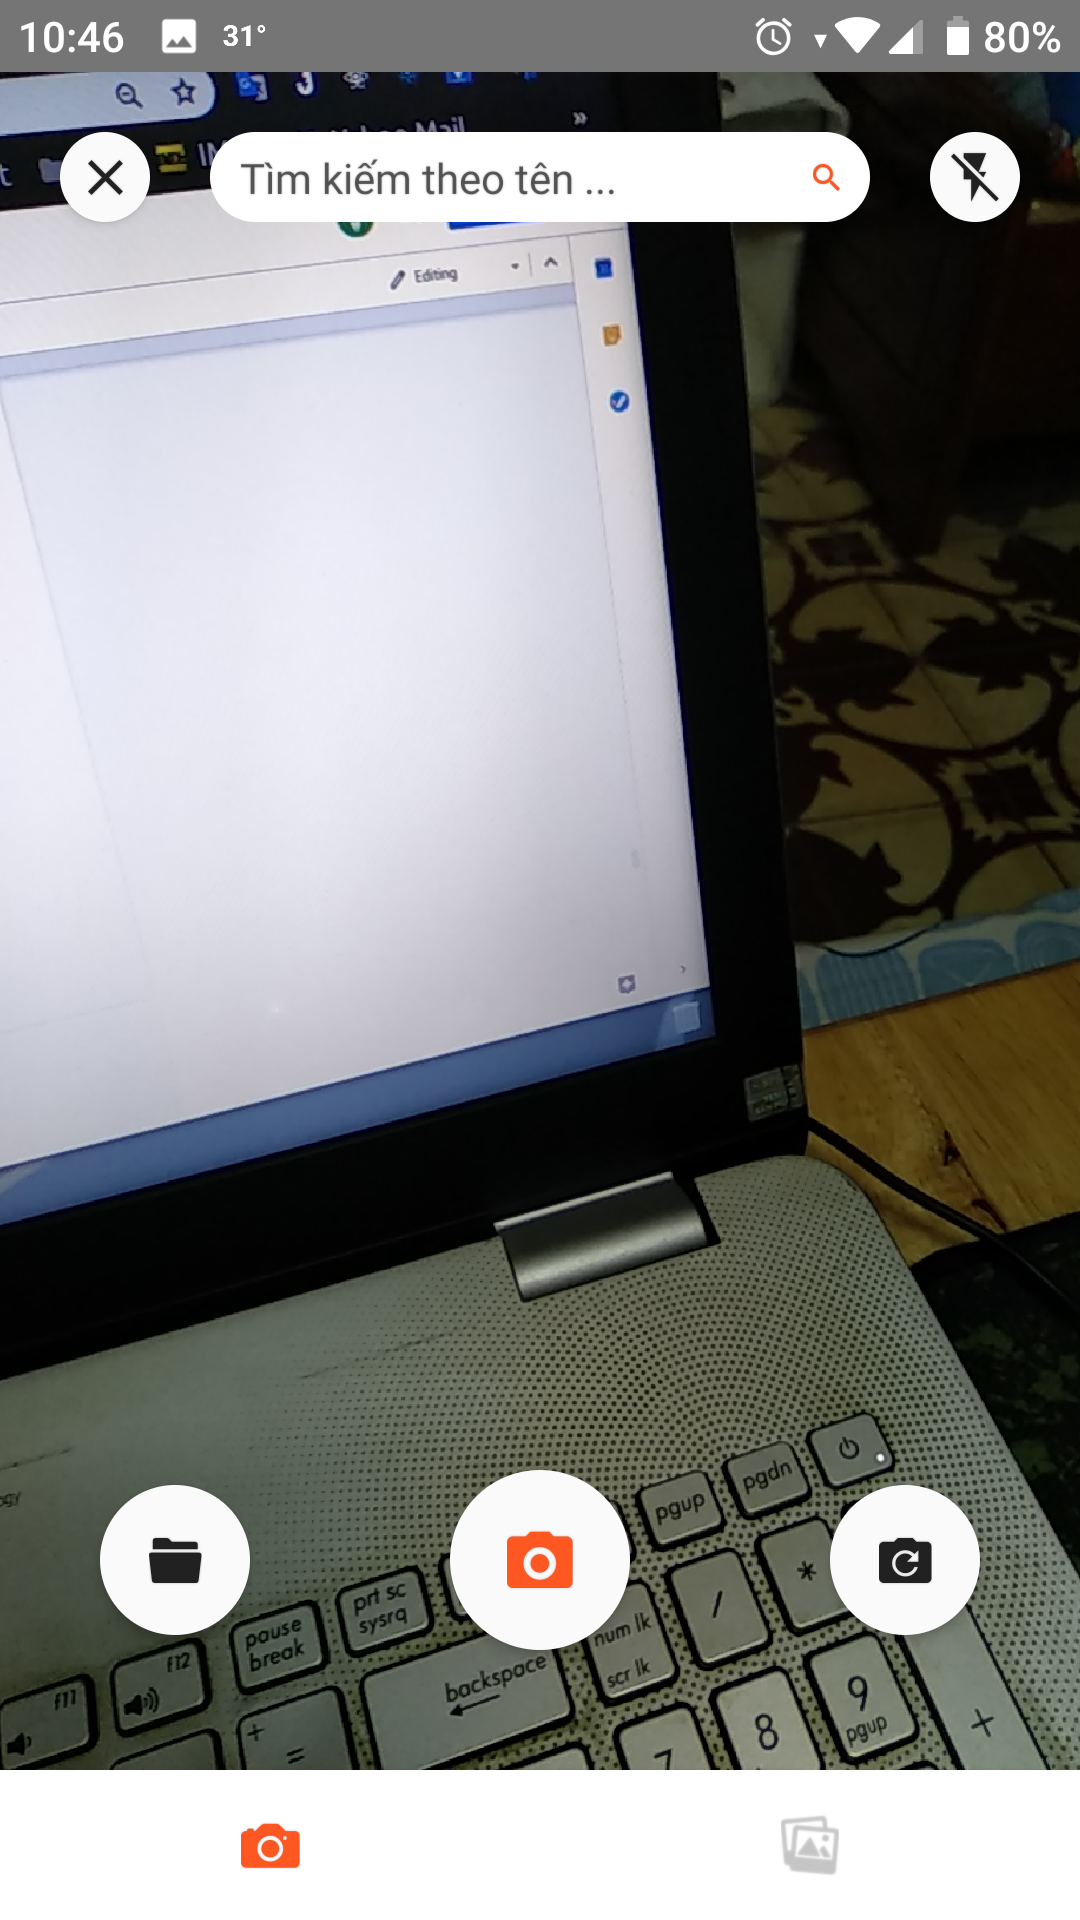
\includegraphics[scale=0.2]{app_no_flower1}
			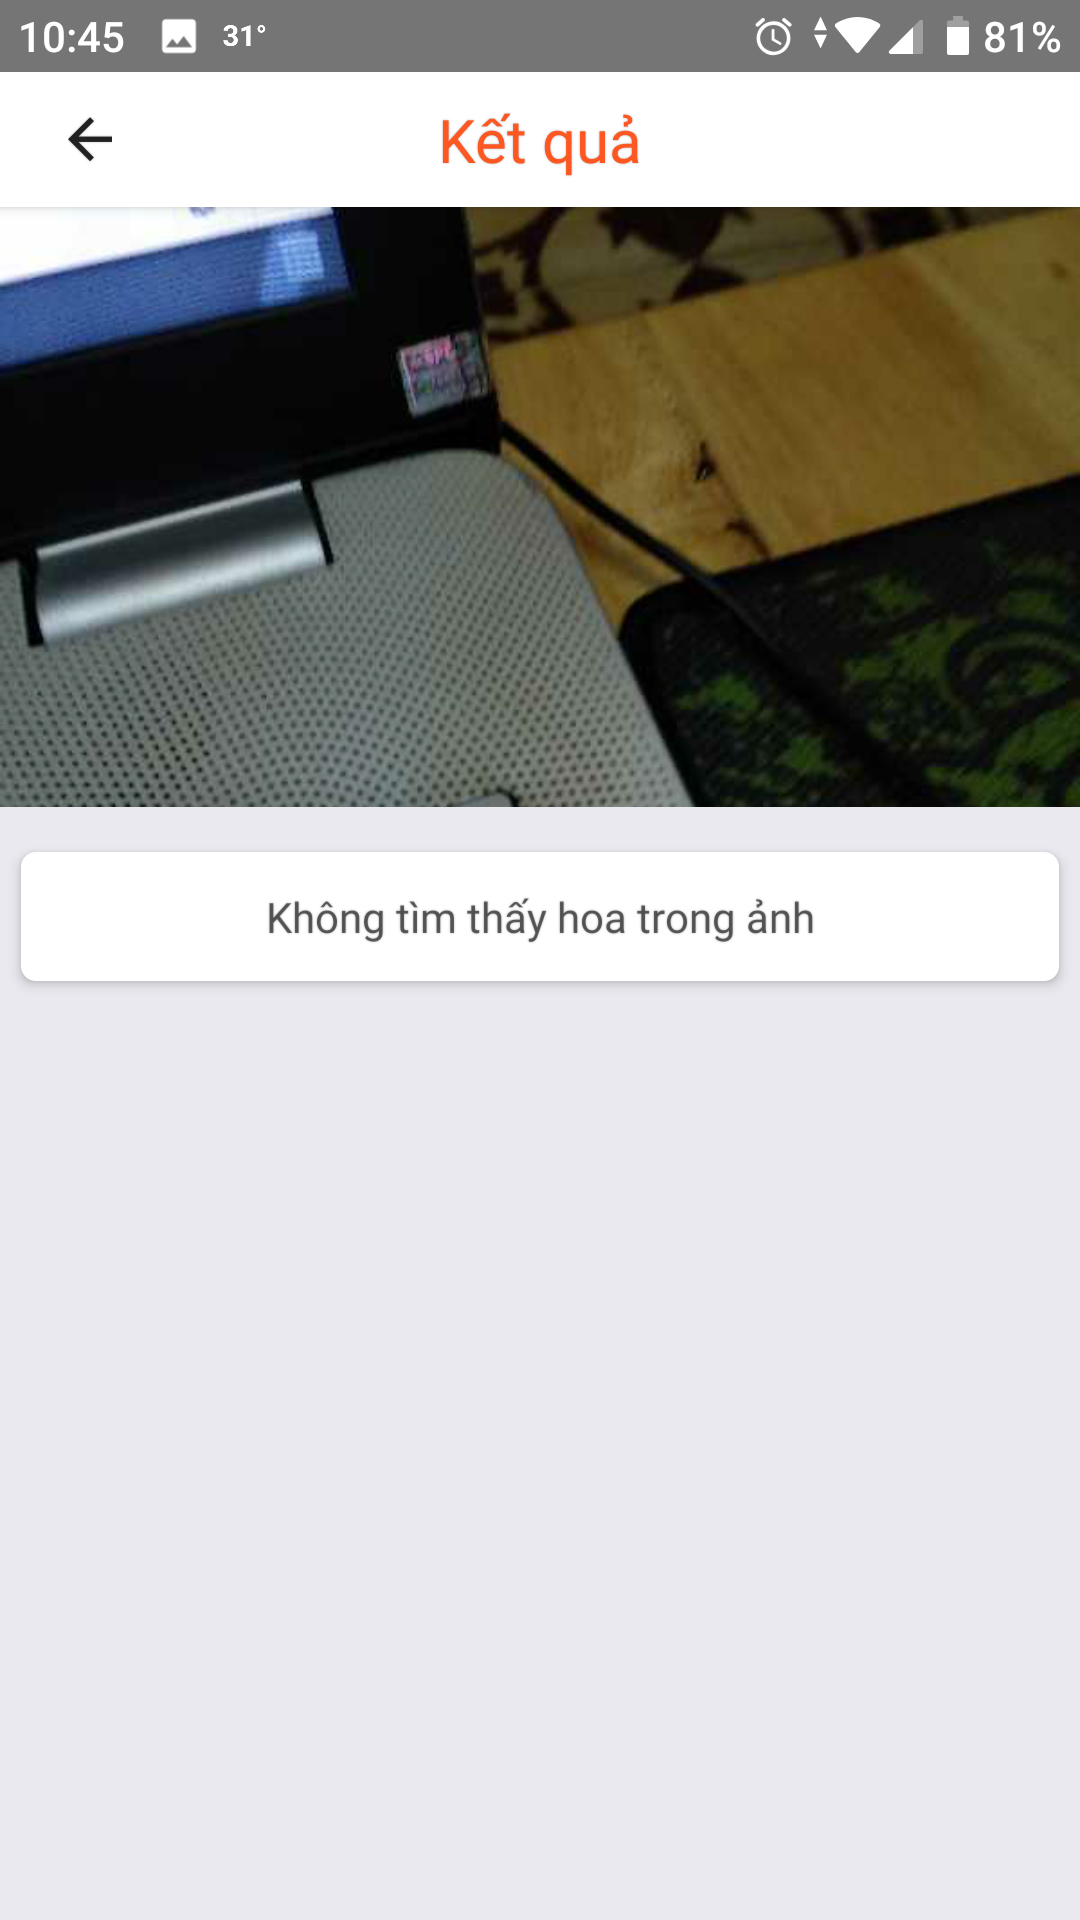
\includegraphics[scale=0.2]{app_no_flower2}
			\caption{Hình ảnh giao diện của ứng dụng khi không phát hiện hoa trong ảnh.}
			\label{fig:app_no_flower}
		\end{figure}

		\newpage
		Chức năng tìm kiếm bằng tên sẽ tìm kiếm theo từ khóa mà bạn nhập vào. Từ khóa bạn nhập có thể là tên tiếng Việt, tiếng Anh, hoặc tên tiếng Latin.
		Khi bấm vào xem chi tiết từng loài hoa ta sẽ có các thông tin sau
		\begin{figure}[h]
			\centering
			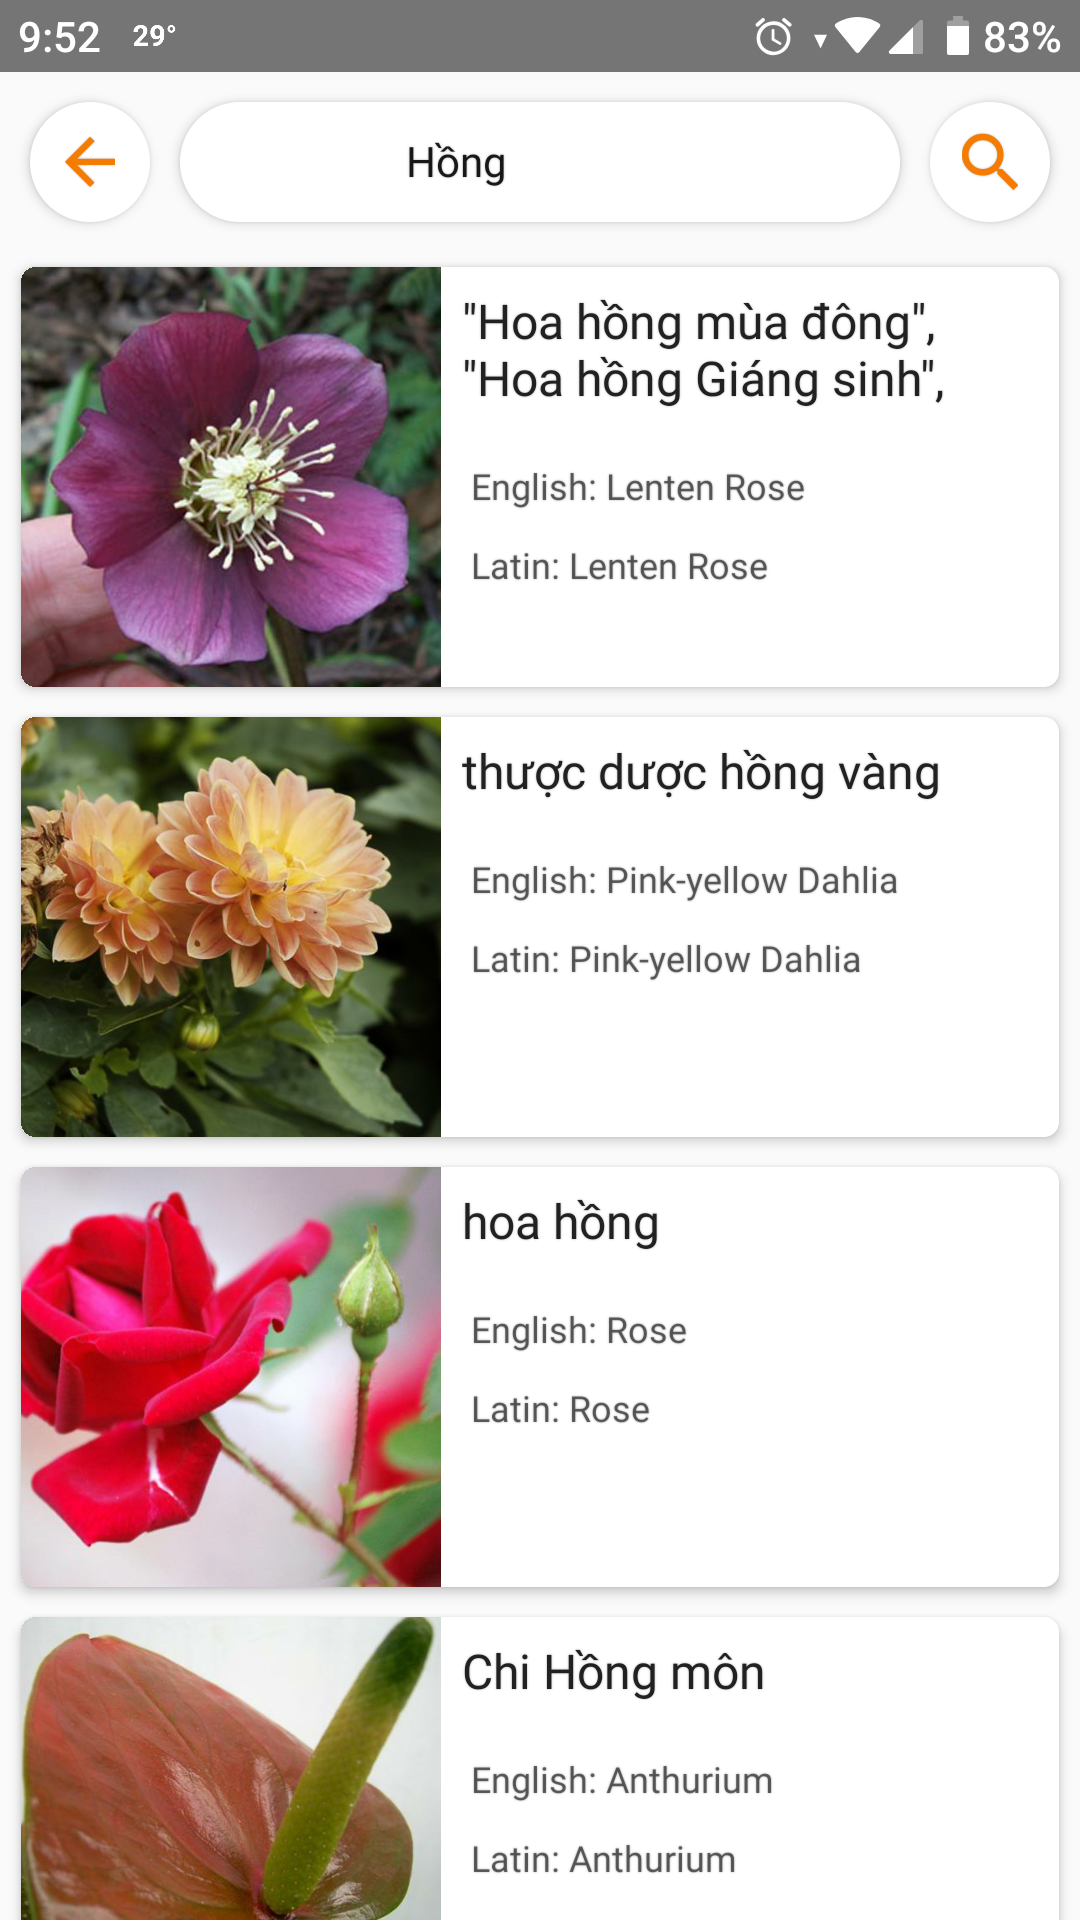
\includegraphics[scale=0.2]{app_search_name}
			\caption{Hình ảnh giao diện tìm kiếm bằng tên.}
			\label{fig:app_search_name}
		\end{figure}
		
		\newpage
		Ở giao diện chi tiết loài hoa tôi có nêu ra tên của loài hoa đó theo tiếng Việt, tiếng Anh, và tên Latin. Đồng thời phía dưới đó chính là đặc điểm của loài hoa đó bao gồm:Đặc điểm chung của loài hoa, đặc điểm sinh trưởng, cách trồng và chăm sóc cây, và ý nghĩa của tên loài hoa.

		Bên cạnh chức năng xem chi tiết đặc điểm của loài hoa là chức năng xem các ảnh tương tự của loài hoa, các ảnh ở đây là các ảnh trong bộ cơ sở dữ liệu.
		\begin{figure}[h]
			\centering
			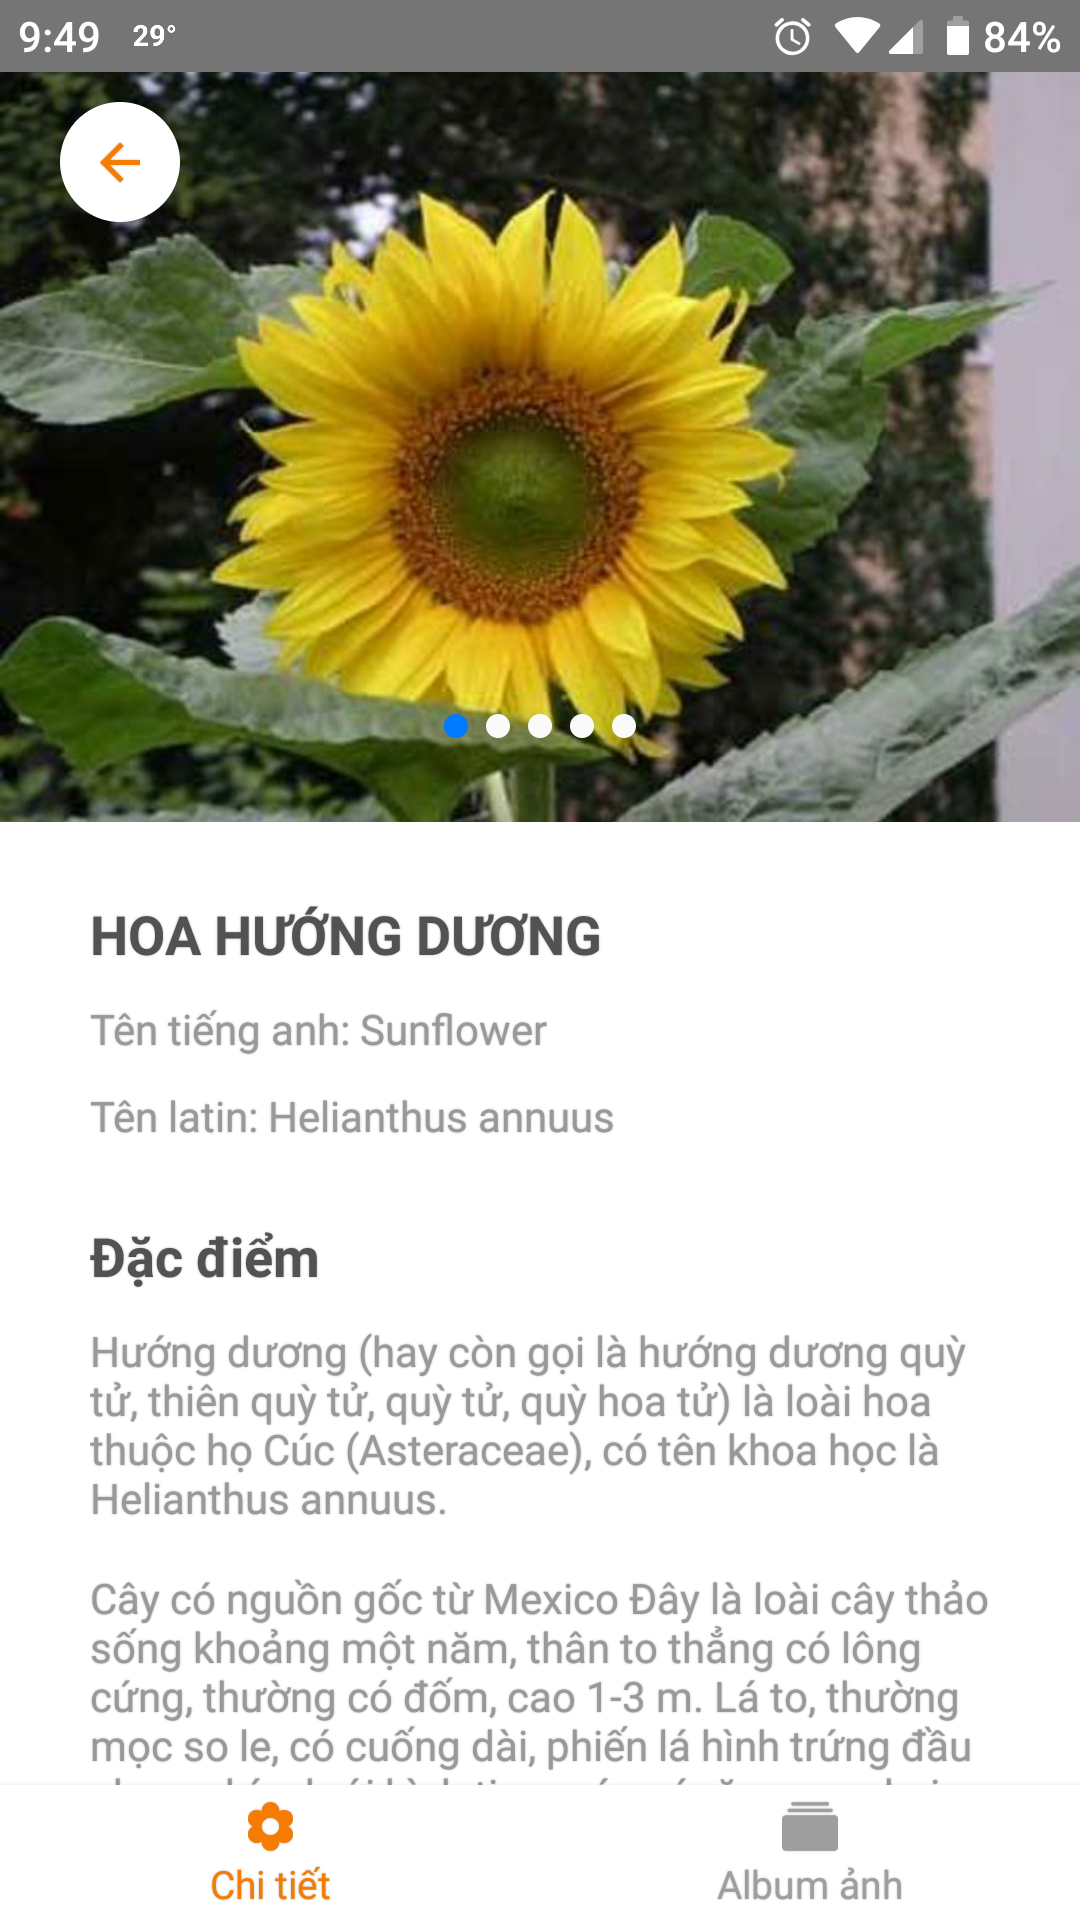
\includegraphics[scale=0.18]{app_detail1}
			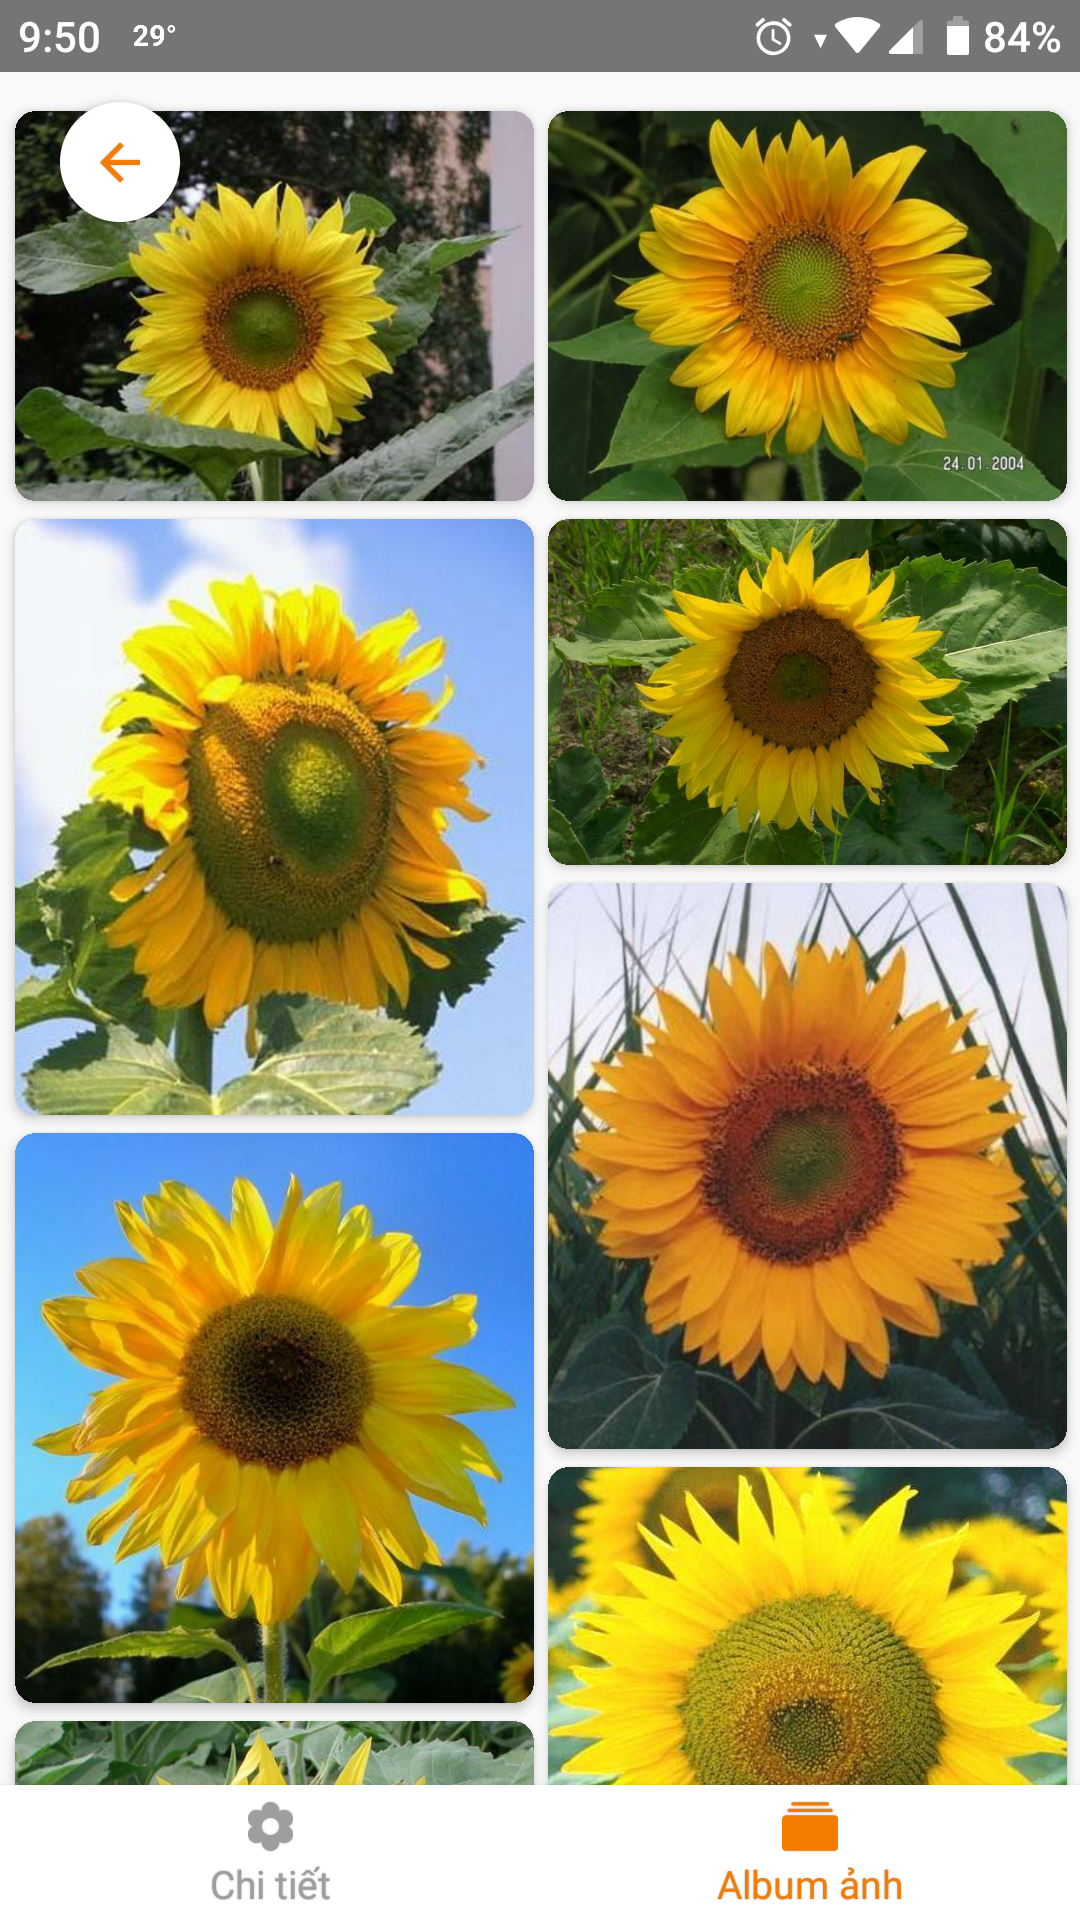
\includegraphics[scale=0.18]{app_detail2}
			\caption{Hình ảnh giao diện chi tiết loài hoa.}
			\label{fig:app_detail}
		\end{figure}


		\newpage
		Chức năng xem lại các ảnh của bản thân, bạn có thể nhìn thấy danh sách các ảnh mà mình đã từng tìm kiếm. Đồng thời cũng có thể nhìn thấy danh sách các ảnh mà do người dùng khác tìm kiếm. 
		\begin{figure}[h]
			\centering
			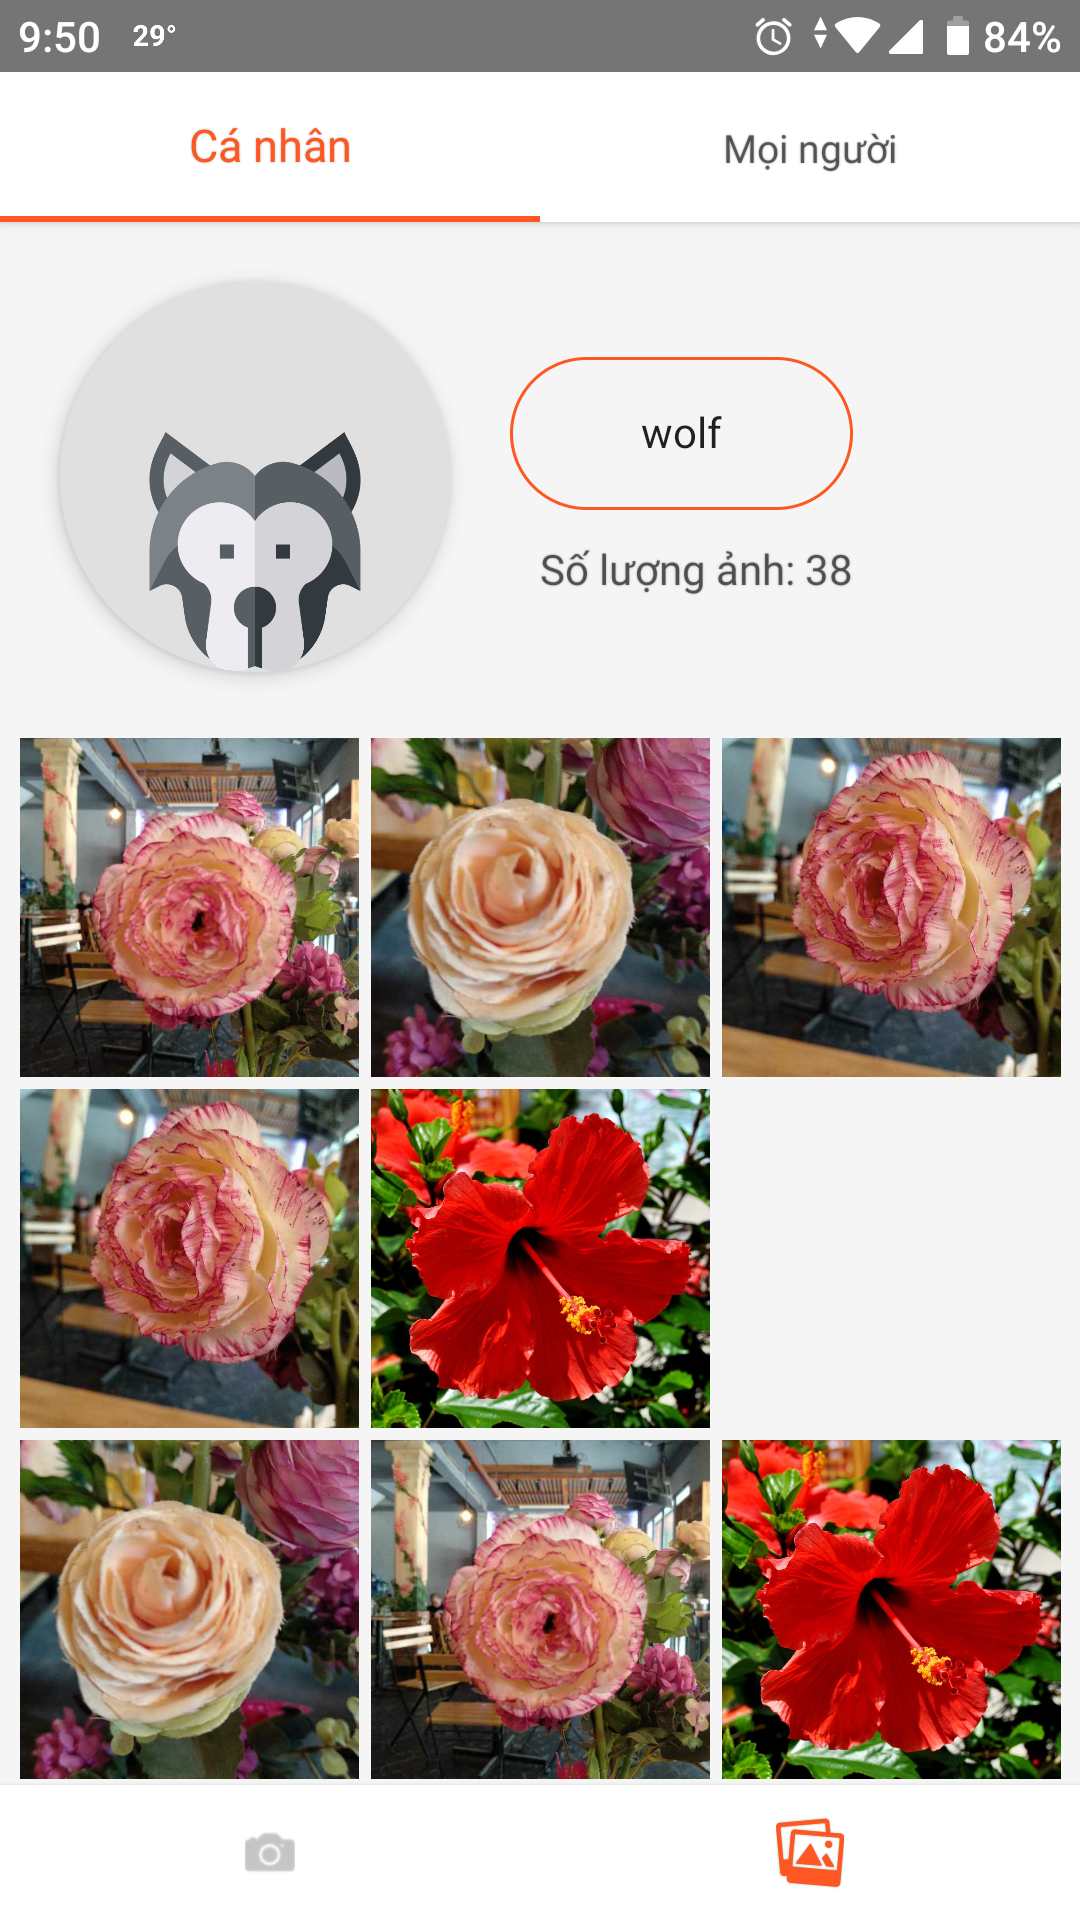
\includegraphics[scale=0.2]{app_profile}
			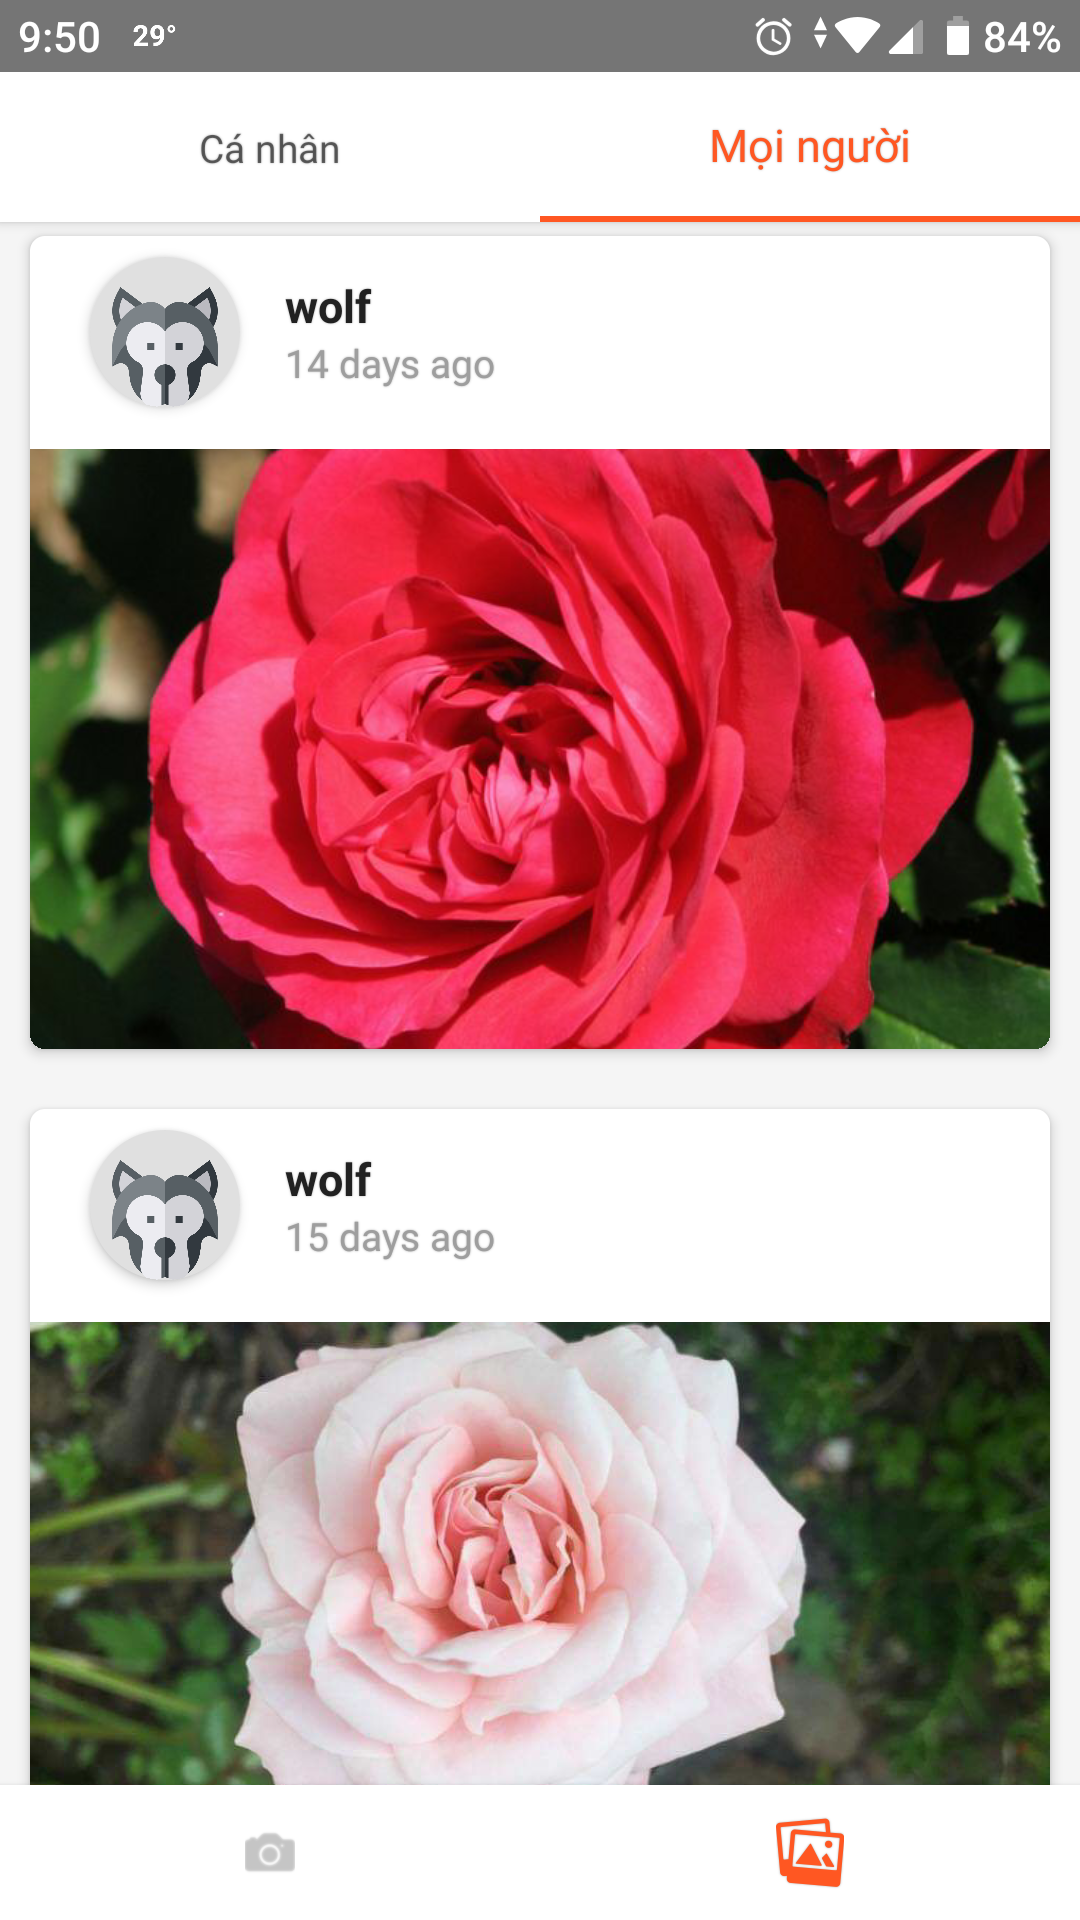
\includegraphics[scale=0.2]{app_social}
			\caption{Hình ảnh giao diện xem lại các ảnh của bản thân và mọi người.}
			\label{fig:app_profile}
		\end{figure}

		\newpage
		Mỗi bức ảnh khi bấm vào ta đều có thể để lại bình luận về loài hoa đó cũng như chia sẻ kinh nghiệm bản thân về cách trồng cũng như chăm sóc loài hoa cho mọi người cùng biết. Đồng thời đưa ra kết quả nhận dạng loài hoa mà ứng dụng đã phản hồi.

		\begin{figure}[h]
			\centering
			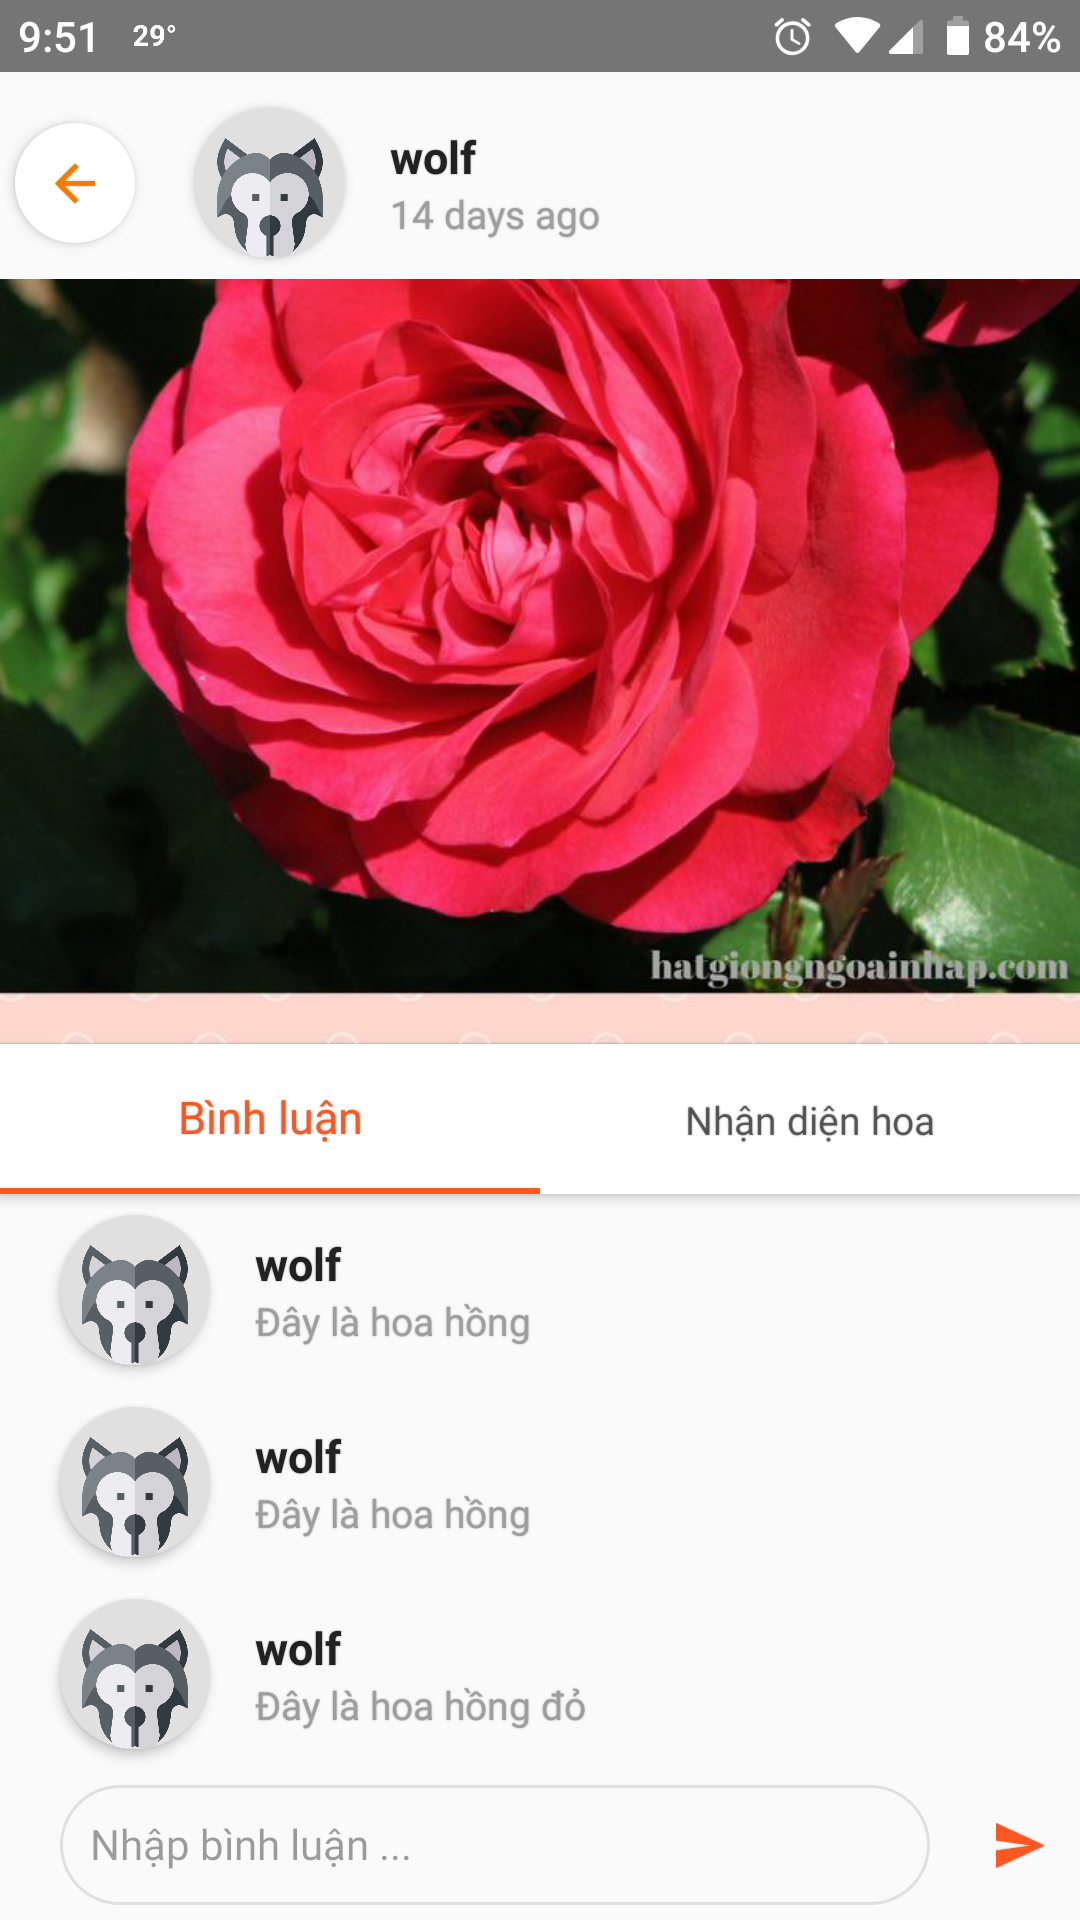
\includegraphics[scale=0.2]{app_comment}
			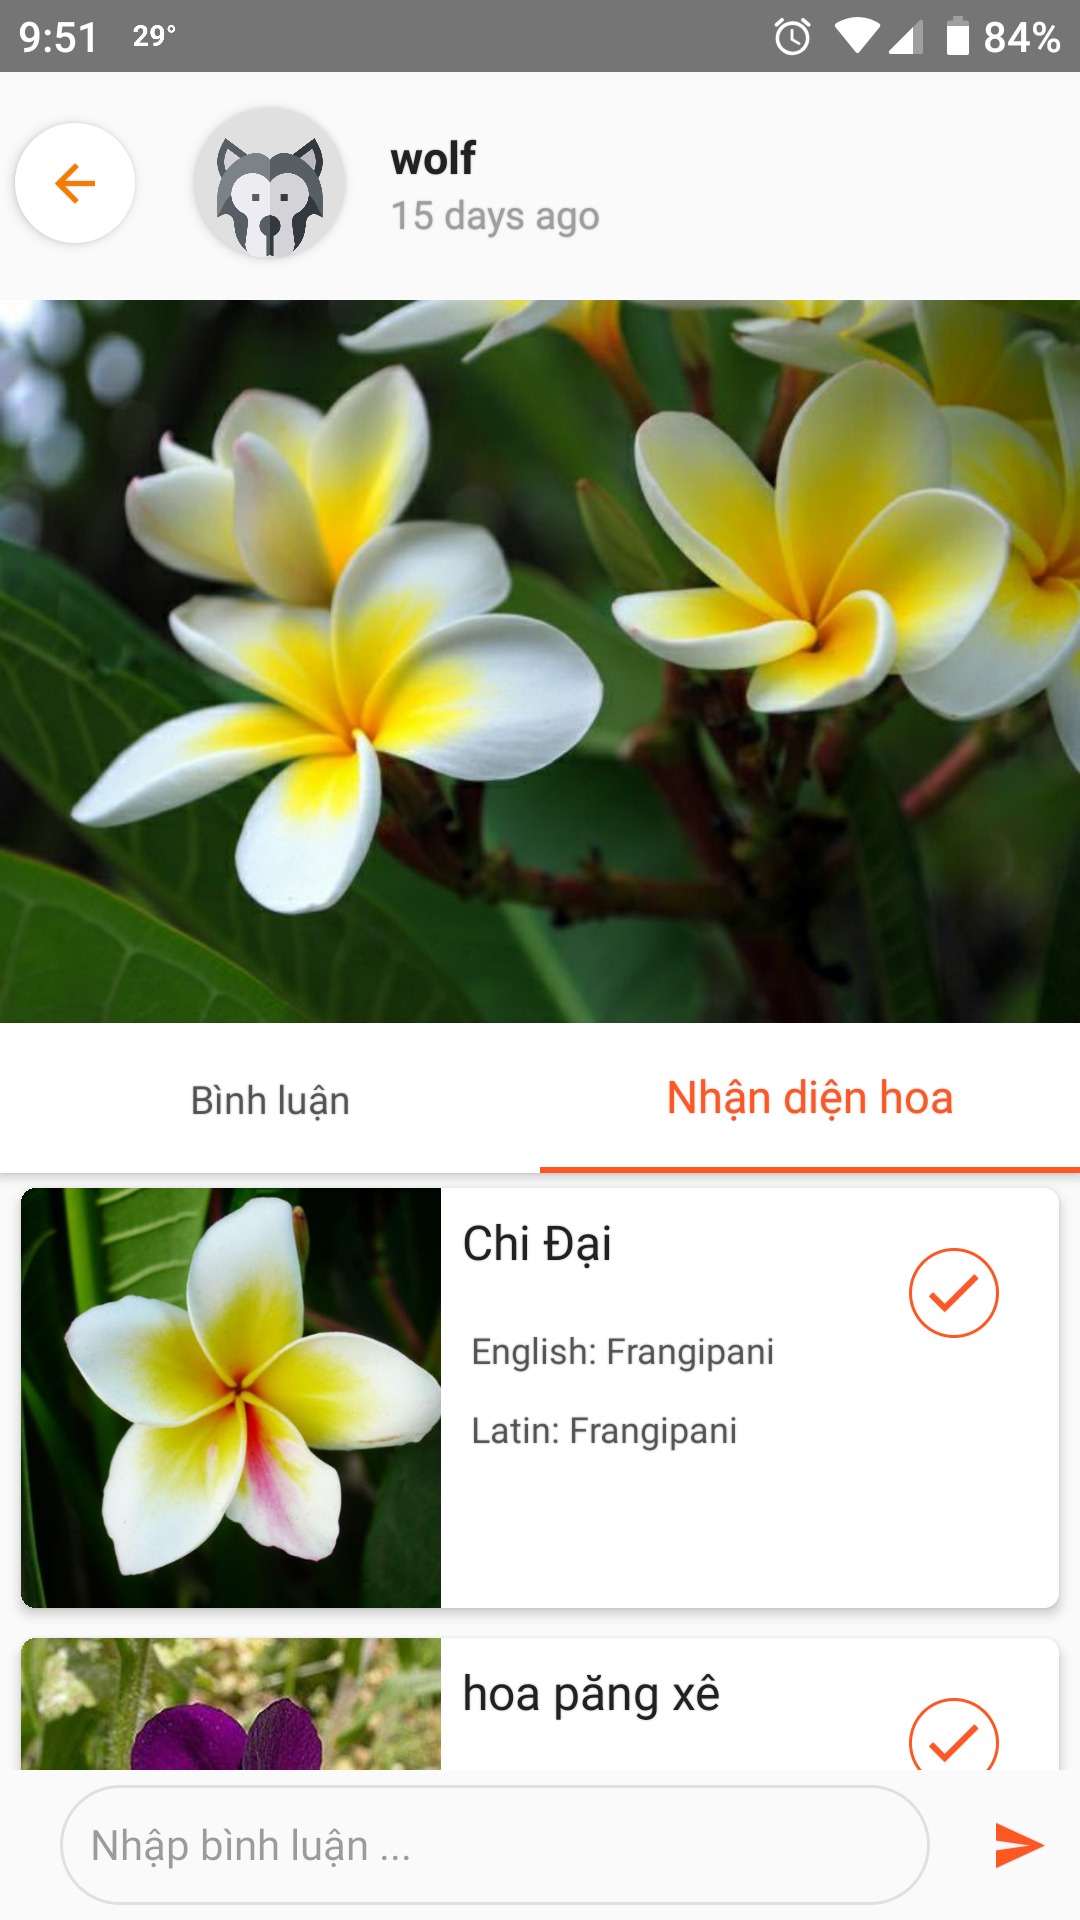
\includegraphics[scale=0.2]{app_comment2}
			\caption{Hình ảnh giao diện xem nhận xét của mọi người.}
			\label{fig:app_comment}
		\end{figure}

		\newpage
		\section{Kết quả của mô hình phát hiện hoa.}
		Dưới đây là kết quả độ chính xác khi phát hiện các loài hoa.
		\begin{table}[h]
			\centering
			\caption{Bảng danh sách các loài hoa phổ biến ở Việt Nam có trong bộ dữ liệu ảnh chụp thực tế}
			\label{tbl:table ket qua cua Nilsback08}
			\begin{tabular}{|c|l|c|}
				\hline
				\textbf{STT} & \textbf{Thuật toán phân loại}& \textbf{Độ chính xác phân loại (\%)} \\ \hline
				1   & SVM & 98.6 \\ \hline   			
			\end{tabular}
		\end{table}



		\section{Kết quả của mô hình phân loại hoa}
		\subsection{Kết quả sử dụng bộ test Oxford-102}
		Dưới đây là kết quả độ chính xác.

		\begin{table}[h]
			\centering
			\caption{Bảng danh sách các loài hoa phổ biến ở Việt Nam có trong bộ dữ liệu ảnh chụp thực tế}
			\label{tbl:table ket qua cua Nilsback08}
			\begin{tabular}{|c|l|c|}
				\hline
				\textbf{STT} & \textbf{Thuật toán phân loại}& \textbf{Độ chính xác phân loại (\%)} \\ \hline
				1   	& KNN 		& 60.35 \\ \hline
				2	& Random-forest	& 65.51\\ \hline
				3	& SVM		& 78.53\\ \hline
			\end{tabular}
		\end{table}
		Kết quả tốt nhất đạt được là 78.53\% khi sử dụng thuật toán phân loại máy vector hỗ trợ SVM.

		\subsection{Giải thích chi tiết từng thí nghiệm}
		Sử dụng bộ dữ liệu Oxford-102 với tên các bộ dữ liệu được viết tắt:
		\begin{itemize}
			\item \texttt{data\_01:} Bộ dữ liệu huấn luyện.
			\item \texttt{data\_02:} Bộ dữ liệu xác nhận.
			\item \texttt{data\_03:} Một nửa bộ dữ liệu kiểm tra.
			\item \texttt{data\_04:} Bộ dữ liệu kiểm tra.
		\end{itemize}

		\textbf{Thí nghiệm với thuật toán KNN}
		Sử dụng thư viện sklearn có cài đặt sẵn thuật toán k láng giềng gần nhất KNN.
		\begin{lstlisting}
		from sklearn.neighbors import NearestNeighbors

		knn = NearestNeighbors(n_neighbors=1, algorithm='ball_tree')
		knn.fit(all_feature_data, all_label)
		distances, indices = knn.kneighbors(img_feature_vector)
		\end{lstlisting}

		Ở đây độ chính xác của thuật toán được đo bằng kết quả của láng giềng gần nhất (K=1). Tôi có sử dụng phương pháp ảnh mở rộng (image augmentation) cụ thể là lật trái, phải, soi vào gương. Như vậy từ một ảnh ban đầu sau phương pháp này ta sẽ có được 4 ảnh.
		
		Độ chính xác của thuật toán được kiểm tra trên bộ data\_04 như bảng dưới.

		\begin{table}[h]
			\centering
			\caption{Bảng danh sách các loài hoa phổ biến ở Việt Nam có trong bộ dữ liệu ảnh chụp thực tế}
			\label{tbl:table ket qua cua Nilsback08}
			\begin{tabular}{|c|l|c|l|l|}
				\hline
				\textbf{STT} 	& \textbf{Phương pháp} 	&\textbf{Bộ dữ liệu}	&\textbf{Phương pháp} 	& \textbf{Độ chính xác} \\ 
					 	&  			&\textbf{huấn luyện}	&\textbf{tăng cường ảnh} & \textbf{phân loại (\%)} \\ \hline

				
				1		& \multirow{4}{*}{KNN} 	& data\_01 			& không		& 54.65 \\ \cline{1} \cline{3-5}
				2		&			& data\_01 			& có		& 55.04	\\ \cline{3-5}
				3		&			& data\_01 + data\_02 		& không		& 60.35	\\ \cline{3-5}
				4		&			& data\_01 + data\_02		& có		& 61.45	\\ \hline
			\end{tabular}
		\end{table}









																																																								
		% chương 5
		\chapter{Kết luận}
		\label{chap:conclusion}
																																																								
		Trong khóa luận này trình bày một ứng dụng nhận dạng tên loài hoa dựa vào ảnh đầu vào trên nền tảng di động. Ứng dụng này được xây dựng với ba mô hình học máy chính: (1) một mô hình phân loại nhị phân để phát hiện có đối tượng hoa trong ảnh hay không, (2) một mô hình nhận dạng tên của loài hoa trong ảnh, và (3) một thuật toán tìm kiếm ảnh tương tự khi hiển thị các ảnh kết quả. 
																																																								
		Ứng dụng được phát triển sử dụng phương pháp sử dụng lại một mô hình học sâu đã được huấn luyện trên bộ dữ liệu lớn khác để trích xuất dữ liệu của ảnh VGG19 [16]. Thực nghiệm so sánh phương pháp tiếp cận này với các cách trích xuất thuộc tính truyền thống chỉ ra tính khả thi và tiết kiệm của việc sử dụng lại mô hình giữa các bài toán nghiên cứu trong lĩnh vực xử lý ảnh.
																																																								
		Những đóng góp chính của khóa luận là: (1) Việt hoá tên cũng như đặc điểm về sinh trưởng, cách trồng của 102 loài hoa trong bộ dữ liệu Oxford-102, (2) phát triển ứng dụng trên nền tảng di động, và (3) phát triển mô hình phân loại ảnh có hoa hay không với độ chính xác 98.6\% và mô hình nhận dạng tên loài hoa với độ chính xác là 78.56\%.
																																																								
		Hướng phát triển tiếp theo của nghiên cứu là  tìm cách khắc phục các điểm còn hạn chế trong việc nhận dạng hoa như nhận dạng đa chủ thể hoa hay nhận dạng hoa khi mọc cả chùm.															
																																																																						
		\begin{thebibliography}{9}
																																																																																													
			\section*{Tiếng Anh}
																																																																																										
			\bibitem{cia-Nilsback06} 
			Maria-Elena Nilsback and Andrew Zisserman. A Visual Vocabulary for Flower Classification Robotics Research Group, Department of Engineering Science University of Oxford, United Kingdom													
																																																																																													
			\bibitem{cia-Nilsback08}
			Maria-Elena Nilsback and Andrew Zisserman. Automated flower classification over a large number of classes Visual Geometry Group, Department of Engineering Science University of Oxford, United Kingdom
																																																																																										
			\bibitem{cia-ONE}
			Lingxi Xie , Richang Hong , Bo Zhang , and Qi Tian. Image Classification and Retrieval are ONE
																																																																																										
			\bibitem{cia-CNNFeatures off-the-shelf}
			CNN Features off-the-shelf: an Astounding Baseline for Recognition Ali Sharif Razavian Hossein Azizpour Josephine Sullivan Stefan Carlsson CVAP, KTH (Royal Institute of Technology) Stockholm, Sweden
																																																																																									
			\bibitem{cia_5}
			M. Varma and D. Ray. Learning the discriminative power invariance trade-off. In Proc. ICCV, 2007.
																																																																																				
			\bibitem{cia_SIFT}
			D. Lowe. Distinctive image features from scale-invariant keypoints. IJCV, 60(2):91–110, 2004.
																																																																																												
			\bibitem{cia_HOG}
			N. Dalal and B. Triggs. Histogram of oriented gradients for human detection. In Proc. CVPR, volume 2, pages 886–893, 2005.
																																																																																										
			\bibitem{cia_MRF}
			Y. Y. Boykov and M. P. Jolly. Interactive graph cuts for optimal boundary and region segmentation of objects in N-D images. In Proc. ICCV, volume 2, pages 105– 112, 2001.
																																																																																									
			\bibitem{cia_temp1}
			Luca Bertelli. Tianli Yu. Diem Vu Burak Gokturk. Kernelized Structural SVM Learning for Supervised Object Segmentation. Google, Inc.
																																																																																							
			% TODO change this right now
			\bibitem{cia_temp2}
			Luca Bertelli. Tianli Yu. Diem Vu Burak Gokturk. Kernelized Structural SVM Learning for Supervised Object Segmentation. Google, Inc.
																																																																																							
			\bibitem{cia_image_augmentation_1}
			L. Perez and J. Wang. The effectiveness of data augmentation in image classification using deep learning. arXiv preprint arXiv:1712.04621, 2017
																																																																																				
			\bibitem{cia_MR8}
			M. Varma and A. Zisserman. Cla	ssifying images of materials: Achieving viewpoint and illumination independence. In Proc. ECCV, volume 3, pages 255–271.Springer-Verlag, May 2002.	
																																																																																							
			\bibitem{cia_object_propo_1}
			B. Alexe, T. Deselaers, and V. Ferrari. Measuring the Objectness of Image Windows. TPAMI, 2012.
																																																																																				
			\bibitem{cia_object_propo_2}
			J. Uijlings, K. van de Sande, T. Gevers, and A. Smeulders. Selective Search for Object Recognition. IJCV, 2013.
																																																																																				
			\bibitem{cia_object_propo_3}
			M. Cheng, Z. Zhang, W. Lin, and P. Torr. BING: Binarized Normed Gradients for Objectness Estimation at 300fps. CVPR, 2014.
																																																																																				
			\bibitem{cia_vgg19}
			K. Simonyan and A. Zisserman. Very deep convolutional networks for large-scale image recognition. In ICLR, 2015.
																																																																																				
			\bibitem{cia_image_augmentation_2}
			Marcus D. Bloice, Christof Stocker, Andreas Holzinger. Augmentor: An Image Augmentation Library for Machine Learning. Medical University of Graz Graz, Austria
																																																																																				
																																																																																				
		\end{thebibliography}
																																																																						
\end{document}